\documentclass[a4paper]{scrbook}

\usepackage[utf8]{inputenc}
\usepackage{graphicx}
\usepackage{booktabs}
\usepackage{url}
\usepackage{relsize}
\usepackage[colorlinks=false, pdfborder={0 0 0}]{hyperref}
\usepackage{libertine}
\usepackage{ifthen}
% \usepackage{fancyhdr}
\usepackage{listings}
\usepackage{xcolor}
\usepackage{amsmath}
\usepackage{scrhack}


% Define colors
\definecolor{numb}{rgb}{0.58,0,0.82}
\definecolor{punct}{rgb}{0.3,0.3,0.3}
\definecolor{delim}{rgb}{0.6,0.6,0.6}


% Define JSON language for listings
\lstdefinelanguage{json}{
  basicstyle=\ttfamily,
  numbers=left,
  numberstyle=\tiny\color{gray},
  stepnumber=1,
  numbersep=8pt,
  showstringspaces=false,
  breaklines=true,
  frame=lines,
  backgroundcolor=\color{lightgray},
  literate=
   *{0}{{{\color{numb}0}}}{1}
    {1}{{{\color{numb}1}}}{1}
    {2}{{{\color{numb}2}}}{1}
    {3}{{{\color{numb}3}}}{1}
    {4}{{{\color{numb}4}}}{1}
    {5}{{{\color{numb}5}}}{1}
    {6}{{{\color{numb}6}}}{1}
    {7}{{{\color{numb}7}}}{1}
    {8}{{{\color{numb}8}}}{1}
    {9}{{{\color{numb}9}}}{1}
    {:}{{{\color{punct}{:}}}}{1}
    {,}{{{\color{punct}{,}}}}{1}
    {\{}{{{\color{delim}{\{}}}}{1}
    {\}}{{{\color{delim}{\}}}}}{1}
    {[}{{{\color{delim}{[}}}}{1}
    {]}{{{\color{delim}{]}}}}{1},
}

\newcommand{\numb}[1]{\textcolor{blue}{#1}}
\newcommand{\punct}[1]{\textcolor{red}{#1}}
\newcommand{\delim}[1]{\textcolor{orange}{#1}}


%%%%%%%%%%%%%%%%%%%%%%%%%%%%%%%%%%%%%%%%%%%%%%%%%%%%%%%%%%%%%%%%%%%%%%%%%%%%%%%%
% Replace these values
%%%%%%%%%%%%%%%%%%%%%%%%%%%%%%%%%%%%%%%%%%%%%%%%%%%%%%%%%%%%%%%%%%%%%%%%%%%%%%%%
\newcommand{\thesistitleDE}{Erkennung von bösartigem Netzwerkverhalten in Allianz-Unternehmensnetzwerkdaten}
\newcommand{\thesistitleEN}{Detection of Malicious Network Behavior in Allianz Company Network Data}
\newcommand{\student}{Aida Nikkhah Nasab}
\newcommand{\matrnr}{22208964}
 %\newcommand{\stammnr}{234567} % Unset this variable if you only have a (single) matriculation number
\newcommand{\submissiondate}{March 2025}
\newcommand{\supervisor}{Prof.~Dr.~Fischer}
 \newcommand{\secsupervisor}{Zineddine Bettouche} % Unset this variable if no second supervisor is required
\newcommand{\faculty}{Angewandte Informatik}

% Select your course of studies here
%\newcommand{\studies}{Bachelor Cybersecurity}
%\newcommand{\studies}{Bachelor Künstliche Intelligenz}
%\newcommand{\studies}{Bachelor Angewandte Informatik}
\newcommand{\studies}{Master Angewandte Informatik}
%\newcommand{\studies}{Bachelor Elektro- und Informationstechnik}
%\newcommand{\studies}{Master Elektro- und Informationstechnik}
%\newcommand{\studies}{Bachelor Medientechnik}
%\newcommand{\studies}{Master Medientechnik}
%\newcommand{\studies}{Master of Applied Research}

% Select the targeted degree here
%\newcommand{\degree}{Bachelor of Engineering (B.Eng.)}
\newcommand{\degree}{Master of Engineering (M.Eng.)}
%\newcommand{\degree}{Master of Science (M.Sc.)}
%%%%%%%%%%%%%%%%%%%%%%%%%%%%%%%%%%%%%%%%%%%%%%%%%%%%%%%%%%%%%%%%%%%%%%%%%%%%%%%%

\renewcommand*{\UrlFont}{\ttfamily\smaller\relax}

\begin{document}
\pagestyle{headings}
\pagenumbering{roman}
\setkomafont{title}{\huge \scshape}
\begin{titlepage}
\begin{center}
	{\usekomafont{subject}
	Technische Hochschule Deggendorf\\
	Fakultät \faculty\par}
	\vspace{.2cm}
{\Large Studiengang \studies\\}
\vspace{6\baselineskip}
{\Huge\usekomafont{title}\thesistitleDE\par}
\vspace{1cm}
{\Huge\usekomafont{title}\thesistitleEN\par}
\vspace{6\baselineskip}

\usekomafont{publishers}
Masterarbeit zur Erlangung des akademischen Grades:

	\vspace{.2cm}
	\emph{\degree}
	\vspace{.2cm}

an der Technischen Hochschule Deggendorf\\
\end{center}
\vfill
\parbox[t]{.4\textwidth}{\usekomafont{author}
	Vorgelegt von:\\
	\student\\
	Matrikelnummer: \matrnr\par
	\ifdefined\stammnr
	Stammnummer: \stammnr\par
	\fi
	\vspace{\baselineskip}
	Am: \submissiondate\par
}
\hfill
\parbox[t]{.4\textwidth}{\usekomafont{author}
Prüfungsleitung:\\
\supervisor%

\ifthenelse{\equal{\secsupervisor}{}}{}
{%
\vspace{\baselineskip}
Ergänzende Prüfende:\\
\secsupervisor%
}}
\end{titlepage}
\cleardoublepage\par


% Erklärung über die Selbständigkeit der Arbeit
\thispagestyle{empty}
\newcommand{\signature}[1]{%
\bigskip
\noindent
\begin{tabular*}{\linewidth}{lp{3cm}p{1cm} p{6cm}}
Deggendorf, & \dotfill & & \dotfill \\
& {\footnotesize Datum} & & {\centering \footnotesize #1}
\end{tabular*}
}

\begin{minipage}[b]{.5\linewidth}
	\Large\textbf{Erklärung}
\end{minipage}
\begin{minipage}[b]{.5\linewidth}
	
\includegraphics[width=\linewidth]{../Thesis_Docs/sources/THD_Logo.pdf}
\end{minipage}

\bigskip

Name des Studierenden: \quad \student

\bigskip
Name des Betreuenden: \quad \supervisor

\vspace{.7cm}
Thema der Abschlussarbeit:

\vspace{.5em}
{\def\\{\relax\ifhmode\unskip\fi\space\ignorespaces}
\thesistitleDE
}\dotfill

\vspace{.5em}
\dotfill

\vspace{.5em}
\dotfill

\vspace{.5em}
\dotfill

\begin{enumerate}
	\item Ich erkläre hiermit, dass ich die Abschlussarbeit gemäß § 35 Abs.~7 RaPO (Rahmen\-prüf\-ungs\-ordnung für die Fachhochschulen in Bayern, BayRS 2210-4-1-4-1-WFK)  selbständig  verfasst,  noch  nicht  anderweitig  für Prüfungszwecke  vorgelegt,  keine  anderen  als  die  angegebenen  Quellen  oder Hilfsmittel  benutzt  sowie  wörtliche  und  sinngemäße  Zitate  als  solche gekenn\-zeichnet habe.

		\signature{Unterschrift des Studierenden}

	\item  Ich  bin  damit  einverstanden, dass die von  mir angefertigte  Abschlussarbeit über die Bibliothek der Hochschule einer breiteren Öffentlichkeit zugänglich gemacht wird:
		\begin{itemize}
			\item[$\bigcirc$] Nein
			\item[$\bigcirc$] Ja, nach Abschluss des Prüfungsverfahrens
			\item[$\bigcirc$] Ja, nach Ablauf einer Sperrfrist von \ldots Jahren.
		\end{itemize}

		\signature{Unterschrift des Studierenden}
\end{enumerate}

\noindent
\hrulefill

{\centering{\footnotesize Bei Einverständnis des Verfassenden vom Betreuenden auszufüllen:}}

{\flushleft

Eine Aufnahme eines Exemplars der Abschlussarbeit in den Bestand der Bibliothek und die Ausleihe des Exemplars wird:

\begin{itemize}
	\item[$\bigcirc$] Befürwortet
	\item[$\bigcirc$] Nicht befürwortet
\end{itemize}

		\signature{Unterschrift des Betreuenden}
}

\cleardoublepage\par


\chapter*{Abstract}
\addcontentsline{toc}{chapter}{Abstract}

This thesis offers a comprehensive examination of the BAYWATCH framework, an advanced system designed for monitoring, detecting, and analyzing data patterns, applied to both real-world and synthetic datasets. The research delves into the theoretical underpinnings of BAYWATCH, outlining its algorithmic architecture, essential components, and the innovative methods it utilizes for real-time anomaly detection and data pattern recognition. Through a systematic evaluation, the study assesses the framework’s performance in controlled experimental settings and its effectiveness in complex, real-world scenarios. The findings indicate that BAYWATCH not only exhibits robust performance and adaptability across diverse data environments but also reveals significant sensitivity to parameter configurations and noise factors present in live datasets. Furthermore, a comparative analysis with existing methodologies highlights BAYWATCH’s strengths and identifies areas for optimization. The insights gained from this research contribute to a deeper understanding of data monitoring systems and offer practical recommendations for future improvements, thereby advancing the application of intelligent data analysis techniques in both academic research and industry practice.


\tableofcontents

\cleardoublepage%
\setcounter{page}{1}
\pagenumbering{arabic}
\chapter{Topical Overview}

\section{Problem Statement}
In the modern world it is important to protect the information and to ensure the security of the network systems as much as it is important for organizations. Like so many others, companies create a large number of user log data every day. It is closely watched for any signs of potential security threats and it is rich with potential insights. However, as cyber attacks become more sophisticated and complex especially APTs, there is the need to have strong and preventive cybersecurity measures in place. The major challenge is how to effectively sort through this huge amount of log data to determine the malicious events and respond to them before they lead to any damage. This research is aimed at enhancing the cybersecurity postures of an organization with a view to detecting APT and other threats early enough in order to protect the network infrastructure.
\section{Methodology Overview}
The methodology followed for this research systematically detects and analyzes the beaconing behavior of network traffic. Several steps are involved in handling this, starting with data collection where both real and artificial datasets have been gathered to ensure that the analysis is substantial.

Advanced data preprocessing on the collected datasets has been carried out in cleaning and preparing the datasets for analysis. It's an important step in which noise and irrelevant information that might distort results can be removed. First, the pre-processing step will ensure that the format of data is appropriate to the analysis step. It would enable better detectability of the beaconing pattern. Thus, the methodology refines the data in order to give more precision to the algorithm in detecting the subtle signs of beaconing behavior that would have been impossible if the approach is relaxed.

\subsection{Data Extraction and Prepration}
These involve gathering large-scale amounts of data across network traffic; it shall further include the variation of attribute varieties such as time stamps, source and destination IP addresses, and URLs visited. The raw data then has an extensive preprocessing step, filtering out irrelevant information, normalizing the data format, and filling in missing values; thus, after the cleaning is performed, structured data will come forth for advanced analytics. The various analytical techniques used to become more familiar with the data will explain how these URLs would behave on a certain day. The different analyses possible on the data can reveal the pattern, anomalies, and trends hidden in this dataset, and that gives interesting insights into the network activity or user behavior. 

\subsection{Whitelist Creation and Filtering}
To enhance the efficiency of the analysis, a whitelist of trusted URLs is created. This whitelist is based on known safe domains and frequently accessed URLs within the organization. By filtering out these trusted URLs, the methodology focuses on potentially suspicious activities, reducing the noise and improving the accuracy of the detection process.

\subsection{Time Interval Analysis}
A critical aspect of the methodology is the analysis of time intervals between successive network requests. By calculating the time differences between consecutive requests to the same URL, the methodology identifies patterns that may indicate beaconing behavior. This analysis helps in distinguishing regular, benign activities from irregular, potentially malicious ones.

\subsection{Bandpass Filtering}
To further refine the analysis, bandpass filtering is applied to the time interval data. This technique isolates specific frequency components within a defined range, effectively filtering out noise and irrelevant fluctuations. The filtered data highlights significant patterns and periodicities, which are crucial for detecting beaconing behavior.

\subsection{Power Calculation and Normalization}
The concept of "power" is introduced to quantify the frequency of network requests. By calculating the power for each URL and normalizing it against the average power, the methodology identifies URLs with unusually high or low request frequencies. This step helps in pinpointing URLs that exhibit abnormal behavior, warranting further investigation.

\subsection{Behavior Detection and Threshold Analysis}
The final stage involves the detection of suspicious behavior based on predefined thresholds. URLs with power values exceeding the threshold are flagged for further scrutiny. This step ensures that only the most significant anomalies are investigated, optimizing the use of resources and enhancing the overall effectiveness of the detection process.

\subsection{Validation and Continuous Improvement}
The methodology is validated using both synthetic and real-world datasets, ensuring its robustness and reliability. Continuous feedback and refinement are integral to the process, allowing the methodology to adapt to evolving network traffic patterns and emerging threats. This iterative approach ensures that the detection system remains effective and up-to-date.

In summary, the methodology combines advanced data analysis techniques with practical filtering and detection strategies to identify beaconing behavior within network traffic. By systematically addressing each stage of the process, the methodology provides a comprehensive framework for enhancing network security and mitigating potential threats.

\section{Research Objectives}
The main goal of this research is to improve the network security of Allianz Company by finding and using better ways to spot and respond to possible cyber threats. The focus is mainly on advanced persistent threats (APTs), which are known for being sneaky and long-lasting. To do this, the research aims to:

\begin{enumerate}
    \item \textbf{Develop Advanced Detection Techniques}: Create methods to identify potential threats early, focusing on the unique behaviors of APTs.
    \item \textbf{Implement Proactive Security Measures}: Establish protocols that enable quicker responses to detected threats, reducing the risk of data breaches.
    \item \textbf{Educate and Train Staff}: Provide training for employees to recognize and respond to potential security threats effectively.
    \item \textbf{Evaluate and Update Security Policies}: Continuously assess and refine the company’s security policies to adapt to new and evolving cyber threats.
\end{enumerate}


\subsection{Research Questions}
The research is guided by the following key questions:
\begin{itemize}
    \item How can beaconing behavior be effectively detected within Allianz Company’s network?
    \item What is the impact of periodicity in network communication on the detection of malicious behavior?
\end{itemize}

\section{Structure of Thesis}
This section outlines the organization of the chapters in this thesis. The structure is designed to systematically address the research objectives and questions outlined above, ensuring a comprehensive understanding of the problem and the proposed solutions.

Chapter 2 provides the  background necessary for understanding the context of this research. It begins with an introduction that sets the stage for the subsequent discussions. This chapter delves into the cybersecurity landscape, highlighting the current state of cybersecurity and the challenges enterprises face. It then explores advanced persistent threats (APTs) and their covert tactics, providing a detailed examination of how these threats operate and the sophisticated methods they employ. Additionally, this chapter discusses enterprise networks, focusing on their structure, functionality, and the inherent vulnerabilities that make them targets for cyberattacks. Finally, it introduces the concept of periodicity in network communication, explaining its relevance to detecting malicious activities.

Chapter 3 is dedicated to a review of related work. It begins with an overview of the BAYWATCH framework, then an exploration of various methods for APT beaconing detection. The chapter then discusses peer-based tracking techniques and presents a systematic review of the literature on APT beaconing detection. Further, it examines the use of DNS logs for malware beaconing detection and the application of AI-driven approaches to identify malicious beaconing. The chapter concludes with a discussion on local periodic communication behavior, providing a comprehensive overview of existing research and highlighting gaps that this thesis aims to address.

Chapter 4 focuses on the methodology adopted for this research. It begins with the design of the proposed method, outlining the theoretical foundation and the rationale behind the chosen approach. This is followed by a detailed description of data extraction and preparation processes, ensuring the data used is both relevant and reliable. The chapter also covers data preprocessing techniques, time interval analysis, and data enhancement methods. Band-pass filtering is introduced as an important step in the methodology, followed by a discussion on the evaluation criteria used to assess the effectiveness of the proposed solution.

Chapter 5 details the implementation of the proposed method. It starts with an explanation of the experimental setup, describing the environment and tools used for the experiments. This chapter also introduces a whitelisting mechanism for URL filtering, aimed at reducing false positives. It then describes the process of average power calculation and the application of band-pass filtering to the data. The chapter concludes with a discussion on behavior detection, explaining how the proposed method identifies malicious activities.

Chapter 6 presents the experiments conducted to validate the proposed method. It includes sections on validation and testing, detailing the procedures and metrics used to assess the performance of the method. An in-depth analysis of the algorithm's output is provided, focusing on the detection of malicious behavior. This chapter aims to demonstrate the efficacy of the proposed method through empirical evidence.

Chapter 7 covers the results and discussions, summarizing the key findings of the research. It provides a critical analysis of the results, discussing their implications and relevance to the field of cybersecurity. This chapter also highlights the contributions of the research, emphasizing how it advances the current state of knowledge.

Chapter 8 concludes the thesis by summarizing the main findings and providing insights into future work. It outlines potential avenues for further research, suggesting how the proposed method can be refined and extended. This chapter aims to provide a comprehensive conclusion to the thesis, tying together the various elements and emphasizing the significance of the research.
In summary, the structure of this thesis is designed to provide a logical and coherent progression from background information and related work to methodology, implementation, experiments, and results, culminating in a comprehensive conclusion and suggestions for future research.
\chapter{Background}
This chapter provides the  background necessary for understanding the context of this research. It begins with an overview of the cybersecurity landscape, emphasizing the current state, emerging trends, and persistent challenges faced by organizations. It then explores Advanced Persistent Threats (APTs) and their sophisticated, covert tactics that pose significant risks to enterprise networks. The discussion also covers the concept of periodicity in network communication, crucial for detecting anomalies in cybersecurity contexts. Finally, the chapter delves into the role of time series databases, with a specific focus on InfluxDB, in managing and analyzing the vast amounts of data generated in cybersecurity operations.

The field of cybersecurity is continually evolving, with new threats emerging as technology advances. Understanding these threats and the strategies to counter them is crucial for protecting sensitive information, ensuring the continuity of operations, and maintaining the integrity of enterprise networks. This chapter lays the foundation for the research by discussing key concepts and technologies relevant to cybersecurity, setting the stage for the detailed analysis and solutions proposed in subsequent chapters.

\section{Cybersecurity Landscape}

The cybersecurity landscape is characterized by a dynamic and increasingly complex environment where various types of cyber threats continually evolve. Organizations across the globe face numerous challenges in protecting their networks, data, and systems from these threats, which range from malware and ransomware to sophisticated nation-state attacks.

Cybersecurity encompasses a wide range of practices, technologies, and strategies aimed at safeguarding information and systems from unauthorized access, damage, or disruption. It involves both proactive measures, such as implementing robust security architectures and practices, and reactive measures, such as incident response and recovery strategies.

\begin{figure}
    \centering
    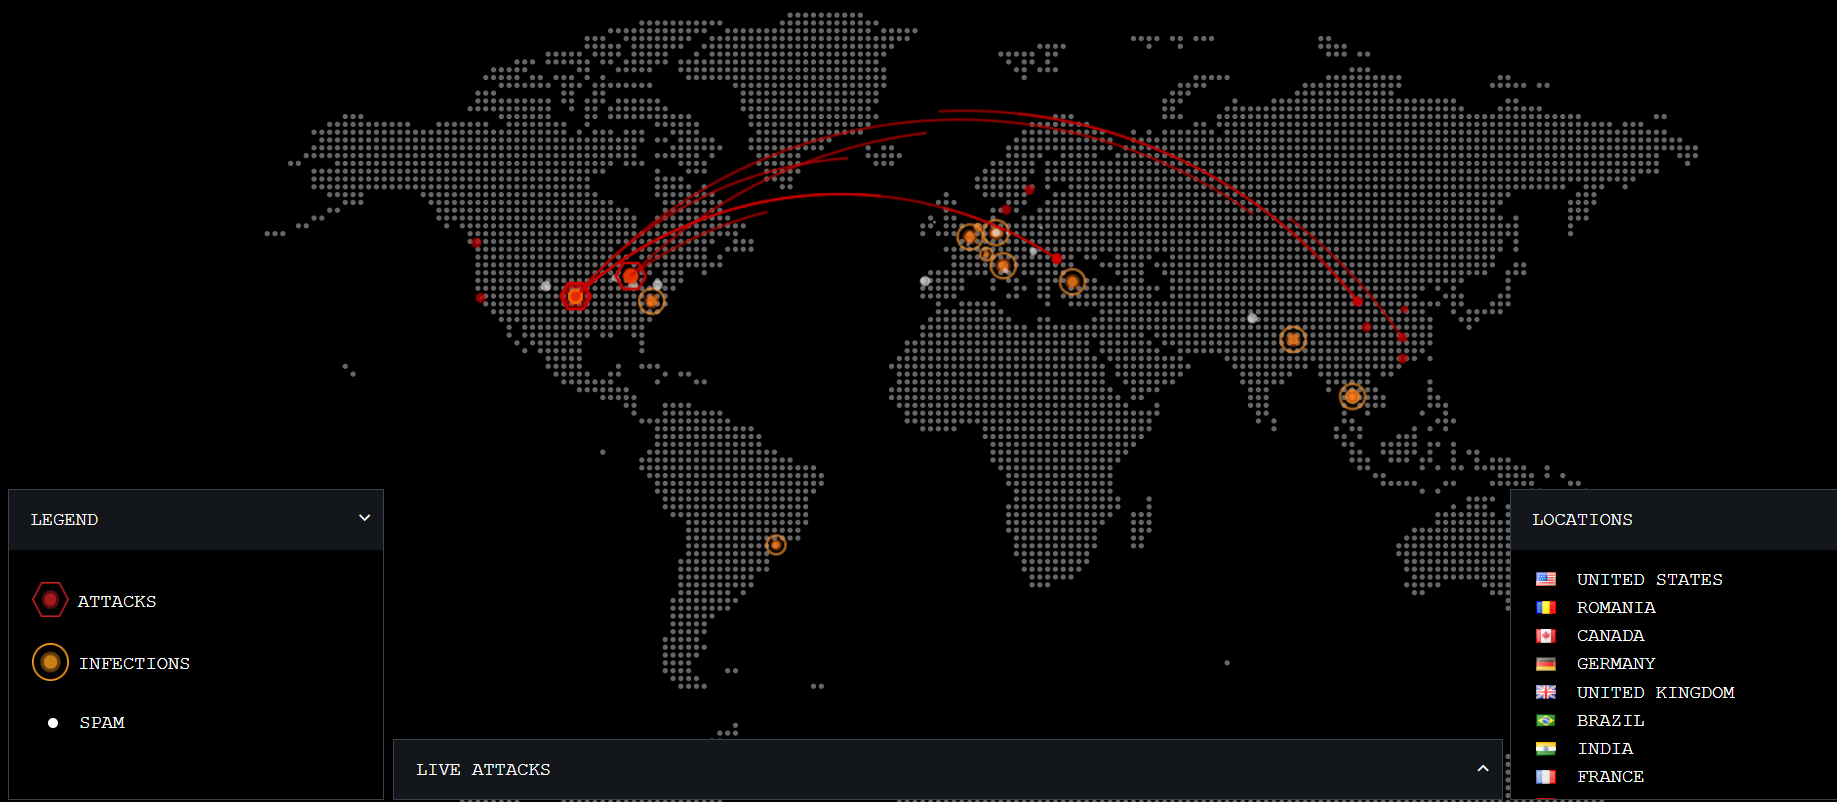
\includegraphics[width=\textwidth]{../Thesis_Docs/media/maps.png}
    \caption{Global cybersecurity threat map \cite{bitdefender}}
    \label{fig:maps}
\end{figure}

Figure \ref{fig:maps} presents a global map of cybersecurity threats, illustrating the widespread nature of these challenges. This visualization highlights regions most affected by various types of cyber attacks, underscoring the global reach and impact of cyber threats.

\subsection{Emerging Trends and Challenges}

The rapid digitization of industries, the increasing reliance on cloud services, and the proliferation of Internet of Things (IoT) devices have significantly expanded the attack surface for cyber threats. These developments, while beneficial, have introduced new vulnerabilities that attackers are quick to exploit. Additionally, the rise of ransomware as a service (RaaS) and the growing sophistication of phishing attacks reflect the evolving threat landscape.

Another significant challenge is the shortage of skilled cybersecurity professionals, which hampers the ability of organizations to effectively defend against these threats. This gap is exacerbated by the complexity of modern networks and the need for advanced tools and techniques to detect and mitigate sophisticated attacks.

\section{Advanced Persistent Threats (APTs) and Covert Tactics}

Advanced Persistent Threats (APTs) represent one of the most sophisticated and dangerous forms of cyber attacks. APTs involve prolonged, targeted efforts by attackers, typically state-sponsored or highly organized criminal groups, aimed at stealing sensitive information, disrupting operations, or compromising critical infrastructure. Unlike traditional cyber attacks, which may be opportunistic and short-lived, APTs are characterized by their stealth, persistence, and the significant resources devoted to them.

\begin{figure}
    \centering
    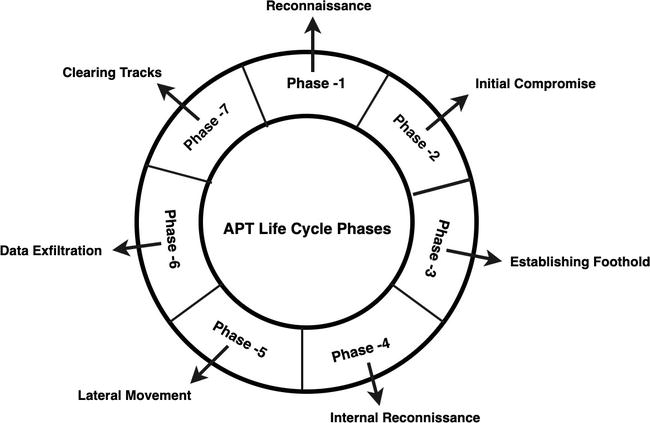
\includegraphics[width=\textwidth]{../Thesis_Docs/media/apt_attack_lifecycle.png}
    \caption{APT attack lifecycle \cite{charan2021dmpt}}
    \label{fig:apt_attack_lifecycle}
\end{figure}

Figure \ref{fig:apt_attack_lifecycle} illustrates the lifecycle of an APT attack, highlighting the various stages involved, from initial reconnaissance to exfiltration of data. Understanding these stages is crucial for developing effective detection and mitigation strategies.

APT actors employ various covert tactics to remain undetected and achieve their objectives. Some of these tactics include:

\begin{itemize}
    \item \textbf{Spear Phishing:} Crafting highly personalized email messages that appear legitimate to the recipient. These emails are designed to trick recipients into clicking on malicious links or attachments, leading to the compromise of their credentials or systems.
    \item \textbf{Zero-Day Exploits:} Exploiting previously unknown vulnerabilities in software or hardware, which have not yet been patched by the vendor. This allows attackers to gain unauthorized access to systems without triggering existing security defenses.
    \item \textbf{Lateral Movement:} After gaining initial access, attackers move within the compromised network, exploring and compromising additional systems to find and exfiltrate valuable data. This tactic often involves the use of legitimate administrative tools to avoid detection.
    \item \textbf{Command and Control (C2):} Establishing a secure communication channel with the compromised systems to remotely control them, issue commands, and exfiltrate data.
\end{itemize}

\subsection{Case Studies of APT Attacks}

Prominent examples of APT attacks include the Stuxnet worm, which targeted Iran's nuclear program, and the SolarWinds breach, which compromised numerous U.S. government agencies and corporations. These cases underscore the potential impact of APTs on national security and global business operations.

\section{Enterprise Networks}

Enterprise networks are the backbone of modern organizations, providing the necessary infrastructure for communication, data sharing, and operational efficiency. However, their complexity and scale make them attractive targets for cyber attackers. Understanding the architecture, components, and vulnerabilities of enterprise networks is  for developing effective cybersecurity strategies.

\begin{figure}
    \centering
    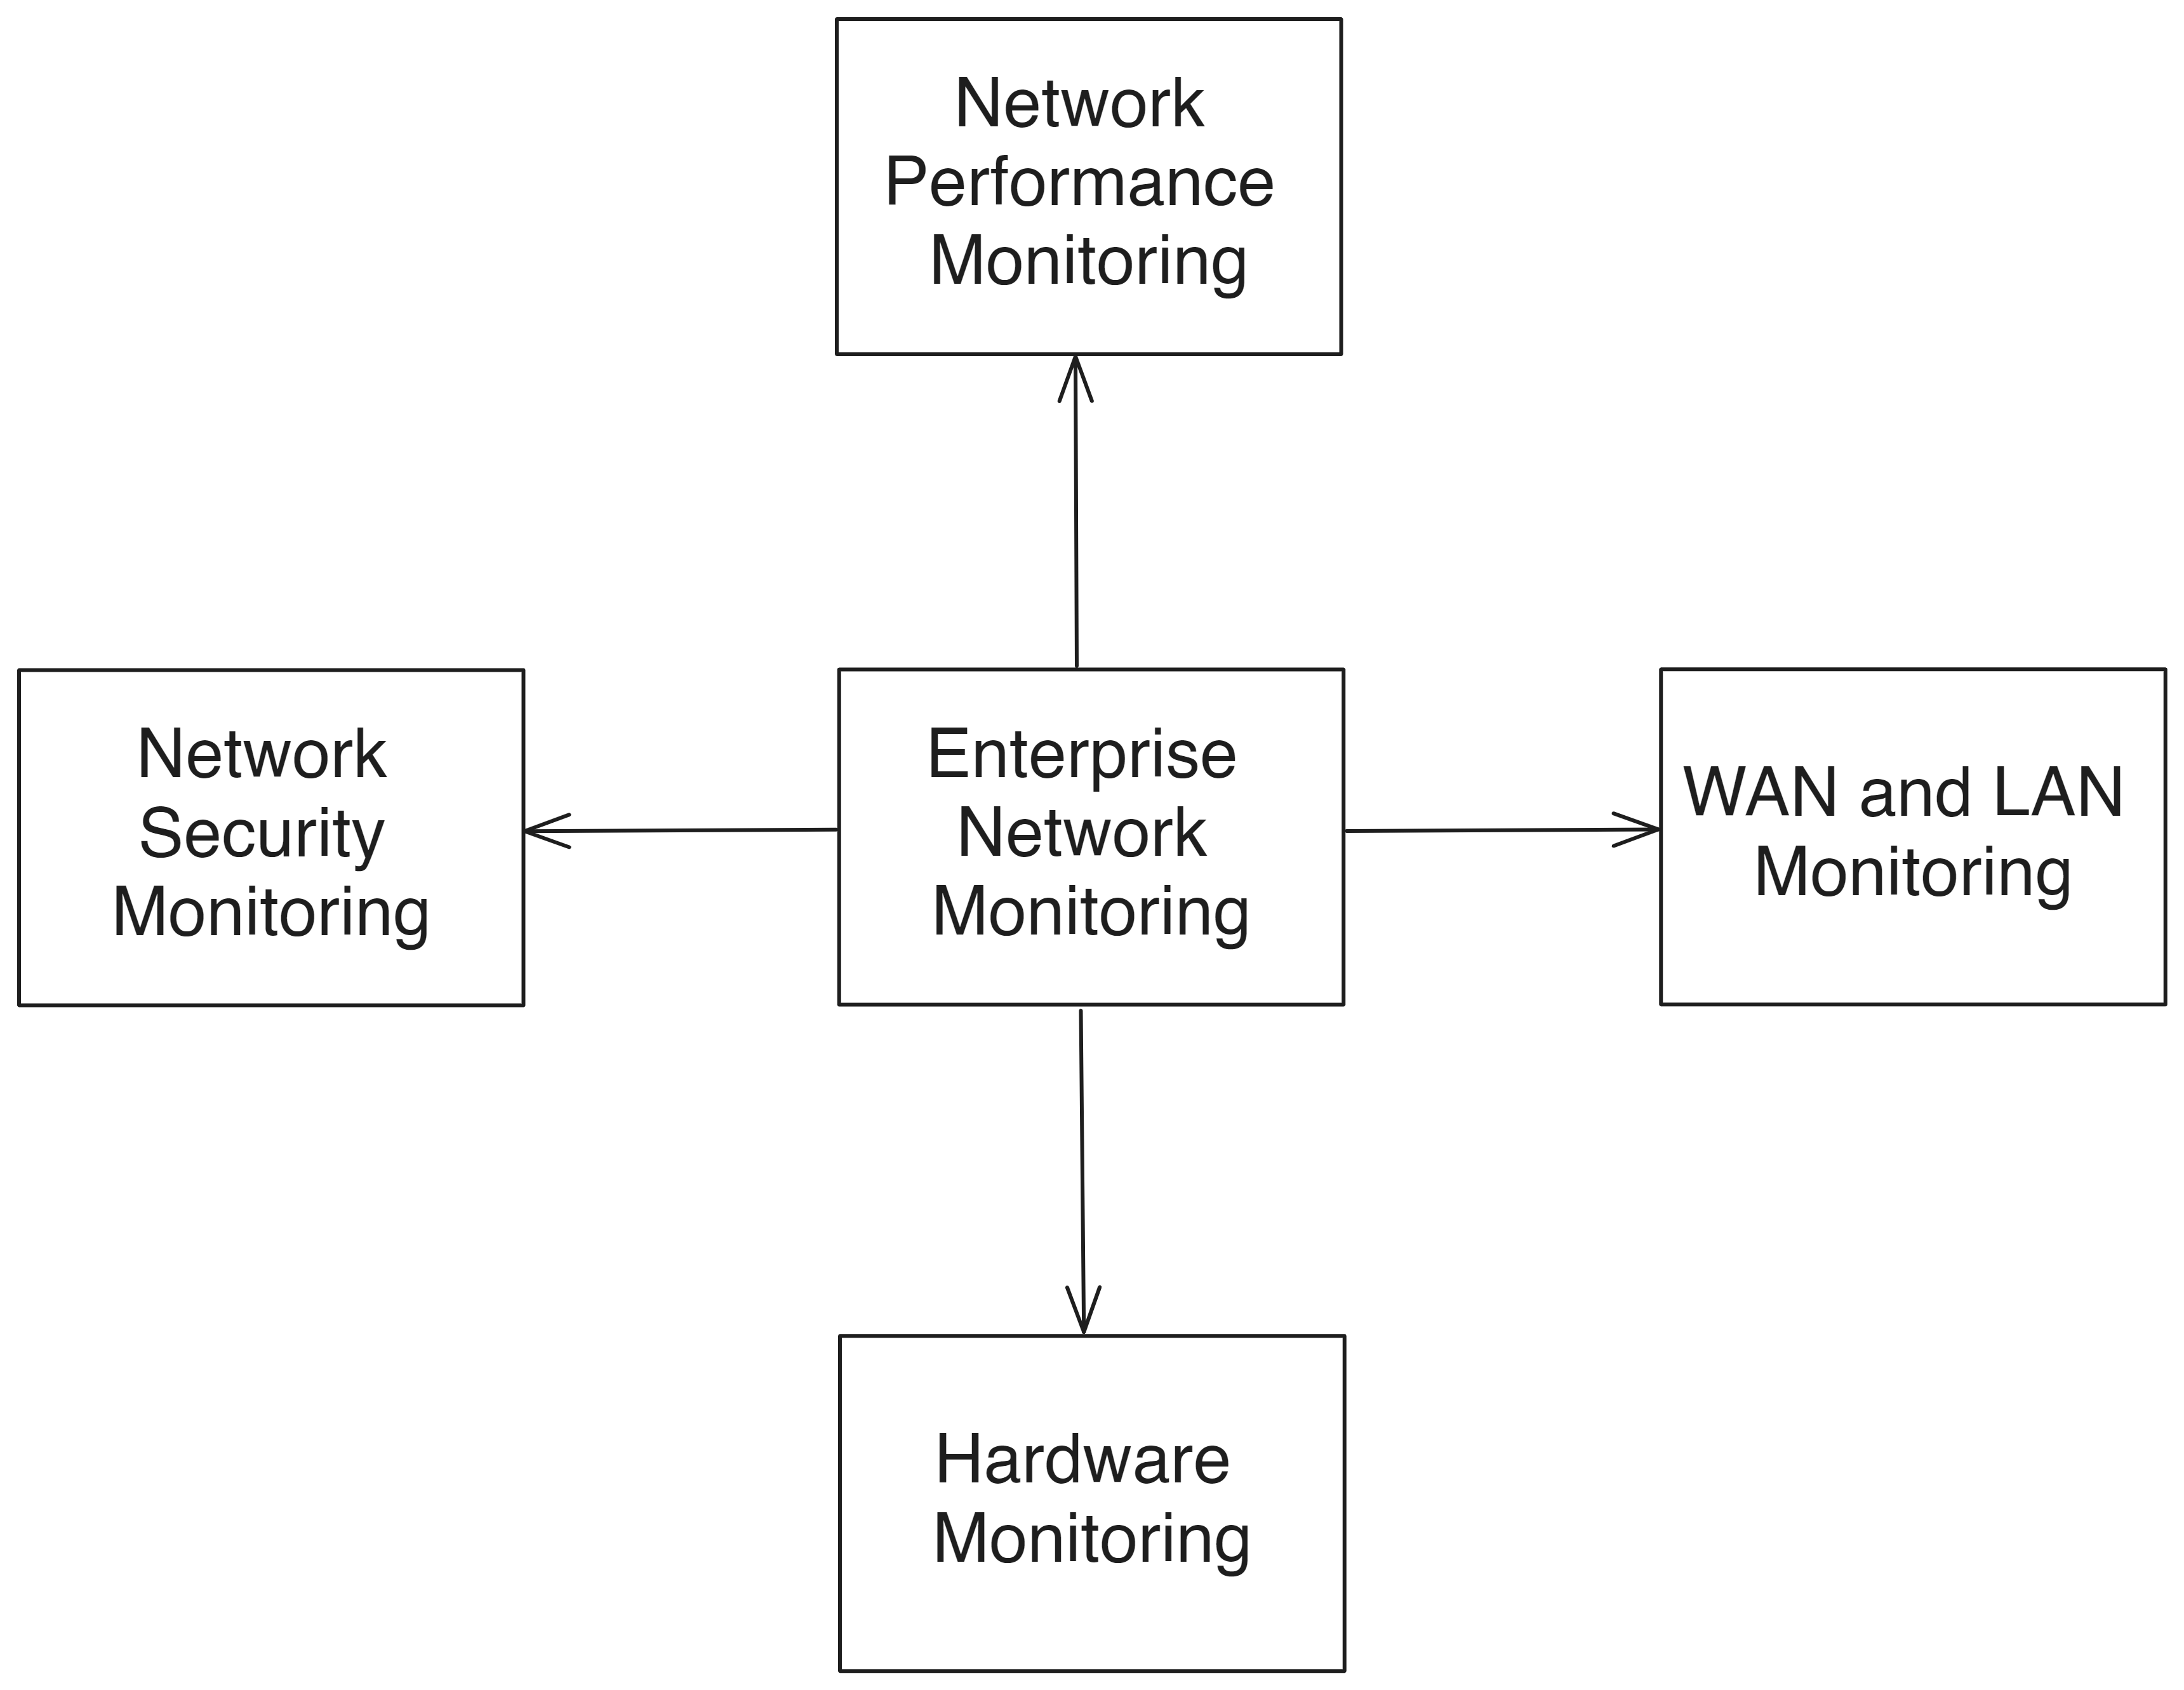
\includegraphics[width=0.7\textwidth]{../Thesis_Docs/media/enterprise_network_diagram.png}
    \caption{Enterprise network diagram}
    \label{fig:enterprise_network_diagram}
\end{figure}

Figure \ref{fig:enterprise_network_diagram} provides a visual representation of an enterprise network, illustrating the various components such as servers, workstations, routers, and communication links, as well as potential points of vulnerability.

\subsection{Key Aspects of Enterprise Networks}

Enterprise networks typically consist of multiple interconnected subsystems, including:

\begin{itemize}
    \item \textbf{Network Architecture:} The physical and logical design of the network, including the layout and interconnection of routers, switches, firewalls, and other network devices. A well-designed architecture enhances security by segmenting the network and controlling traffic flow.
    \item \textbf{Security Protocols:} Protocols such as TLS (Transport Layer Security) and IPSec (Internet Protocol Security) protect data in transit. Additionally, firewalls, intrusion detection/prevention systems (IDS/IPS), and encryption mechanisms are employed to safeguard data and systems.
    \item \textbf{Access Controls:} Policies and technologies that regulate who can access specific data and resources within the network. This includes user authentication, role-based access control (RBAC), and multi-factor authentication (MFA) to ensure that only authorized personnel can access sensitive information.
    \item \textbf{Network Monitoring and Management:} Tools and practices for monitoring network traffic, identifying anomalies, and managing network resources to maintain performance and security.
\end{itemize}

\subsection{Vulnerabilities in Enterprise Networks}

Despite the implementation of robust security measures, enterprise networks remain vulnerable to a variety of threats, including:

\begin{itemize}
    \item \textbf{Insider Threats:} Employees or contractors with legitimate access who misuse their privileges, either maliciously or negligently.
    \item \textbf{Advanced Malware:} Malware is designed to bypass traditional security measures, often delivered through phishing attacks or drive-by downloads.
    \item \textbf{Misconfigurations:} Incorrectly configured devices or systems that leave the network open to exploitation.
    \item \textbf{Supply Chain Attacks:} Attacks that target the software or hardware supply chain, introducing vulnerabilities that can be exploited after deployment.
\end{itemize}

\section{Periodicity in Network Communication}

Periodicity in network communication refers to the recurring patterns observed in network traffic over time. Detecting and analyzing these patterns can provide valuable insights into normal and anomalous behavior within the network. In cybersecurity, periodicity analysis is particularly useful for identifying stealthy activities, such as those conducted by APTs, which may generate periodic communication to maintain control over compromised systems.

\subsection{Importance in Cybersecurity}

Understanding periodicity is crucial for the following reasons:

\begin{itemize}
    \item \textbf{Anomaly Detection:} Deviations from established periodic patterns can indicate the presence of malware or other malicious activities.
    \item \textbf{Traffic Analysis:} Analyzing periodic traffic can help in identifying command and control (C2) communications used by attackers.
    \item \textbf{Resource Optimization:} Periodicity analysis can be used to optimize network resources by predicting traffic loads and adjusting resources accordingly.
\end{itemize}

\section{Time Series Databases}

Time series databases are specialized databases designed to handle time-stamped or time-series data efficiently. This type of data is common in network activity logs, sensor readings, financial transactions, and many other applications where the sequence and timing of data points are critical. Time series databases are optimized for high-frequency data writes and efficient queries over time intervals, making them ideal for use in monitoring, alerting, and anomaly detection in cybersecurity contexts.

\subsection{Characteristics of Time Series Databases}

Time series databases differ from traditional relational databases in several key ways:

\begin{itemize}
    \item \textbf{Time-Optimized Storage:} Data is stored in a way that optimizes retrieval by time, enabling fast queries across large datasets.
    \item \textbf{Efficient Data Compression:} Given the often high volume of data, time series databases employ advanced compression techniques to reduce storage requirements.
    \item \textbf{High Throughput:} They are optimized to handle high-frequency data writes and queries, ensuring efficient data handling even under heavy load.
    \item \textbf{Querying Capabilities:} Time series databases support complex querying over time intervals, which is  for trend analysis and anomaly detection.
\end{itemize}

\subsection{InfluxDB}

InfluxDB is a popular time series database known for its high performance and ease of use. It is optimized for handling large-scale time-series data, providing powerful querying capabilities and efficient storage.

\subsubsection{Key Features of InfluxDB}

\begin{itemize}
    \item \textbf{Time-Optimized Storage:} InfluxDB uses a custom storage engine that efficiently writes and reads time-series data.
    \item \textbf{High Throughput:} It can handle high write and query loads, making it suitable for large-scale monitoring applications.
    \item \textbf{SQL-like Query Language (Flux):} InfluxDB offers a powerful query language that is both easy to learn and capable of complex data manipulations.
    \item \textbf{Retention Policies:} Users can define retention policies to manage data lifecycle, automatically deleting old data to save storage.
    \item \textbf{Integrations:} InfluxDB integrates well with other tools and platforms, supporting various data inputs and outputs.
\end{itemize}

\subsubsection{Applications in Cybersecurity}

InfluxDB can be employed in cybersecurity for:

\begin{itemize}
    \item \textbf{Real-Time Monitoring:} Capturing and analyzing live data to detect anomalies and potential threats.
    \item \textbf{Historical Analysis:} Storing historical data for trend analysis and forensic investigations.
    \item \textbf{Alerting:} Setting up alerts based on specific criteria to notify administrators of suspicious activities.
    \item \textbf{Visualization:} Integrating with visualization tools like Grafana to create dashboards that display network metrics and security insights.
\end{itemize}

\begin{figure}
    \centering
    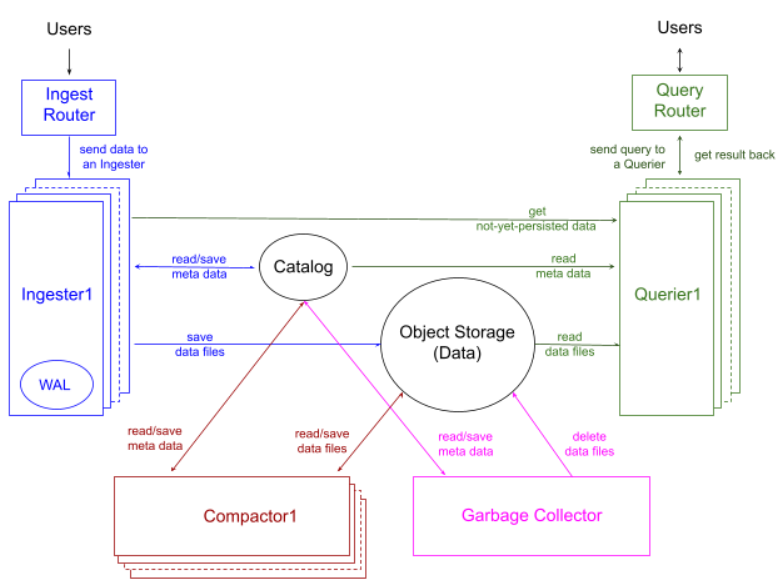
\includegraphics[width=\textwidth]{../Thesis_Docs/media/influxdb_architecture.png}
    \caption{InfluxDB Architecture \cite{influxdb2023}}
    \label{fig:influxdb_architecture}
\end{figure}

Figure \ref{fig:influxdb_architecture} illustrates the architecture of InfluxDB and how data flows through the system, from ingestion to querying and visualization.

\section{Summary}

This chapter has provided a comprehensive overview of the cybersecurity landscape, APTs and their covert tactics, enterprise networks, periodicity in network communication, and time series databases, with a detailed focus on InfluxDB. These foundational topics are  for understanding the subsequent chapters, which will delve deeper into related work, methodology, implementation, experiments, and results. The knowledge gained from this background will inform the development and evaluation of advanced techniques for detecting and mitigating cyber threats in enterprise networks.
\chapter{Related Work}

Hu et al. (2016) proposed BAYWATCH, a robust beaconing detection method designed to identify infected hosts in large-scale enterprise networks \cite{hu2016baywatch}. The method focuses on detecting beaconing behavior, which is commonly exhibited by compromised hosts communicating with external command and control servers. By analyzing network traffic patterns, BAYWATCH can efficiently detect infected devices while minimizing false positives. The system is specifically designed to scale in large enterprise environments, making it suitable for real-world deployment. The authors validate BAYWATCH through extensive evaluation using real-world network traffic, demonstrating its effectiveness in identifying infected hosts and improving network security.

Zhang et al. (2023) introduced a global analysis approach for aggregation-based beaconing detection across large campus networks \cite{zhang2023global}. Their method focuses on detecting beaconing behavior in network traffic by aggregating data from multiple sources within a campus network, which enhances detection accuracy. The approach is designed to scale across large networks and aims to minimize false positives by leveraging aggregation techniques. The authors validate their method through extensive experiments on real-world campus networks, demonstrating its effectiveness in identifying compromised hosts and improving network security in large-scale environments.

Apruzzese et al. (2017) proposed a method for identifying malicious hosts involved in periodic communications \cite{apruzzese2017identifying}. Their approach focuses on detecting abnormal periodic communication patterns in network traffic, which are often indicative of compromised hosts communicating with external servers. The authors introduce a novel technique for identifying such hosts by analyzing the timing and frequency of communication sessions. The proposed method is evaluated through experiments, demonstrating its effectiveness in identifying malicious hosts and enhancing network security by targeting irregular communication patterns.

Seo and Lee (2018) proposed an abnormal behavior detection method to identify infected systems using the APChain algorithm and behavioral profiling \cite{seo2018abnormal}. Their approach focuses on analyzing system behavior to detect deviations from normal activity, which may indicate the presence of malware or compromised systems. The APChain algorithm is used to model and track the behavior of systems, allowing for the identification of anomalous patterns associated with infected hosts. The authors validate their method through experiments, demonstrating its effectiveness in detecting abnormal behaviors and enhancing system security in real-world environments.

Huynh et al. (2016) focused on uncovering periodic network signals of cyber attacks \cite{huynh2016uncovering}. The paper explores how periodic network traffic patterns can indicate cyber attacks, particularly in the context of detecting covert channels used by attackers for command and control. The authors propose a method to identify such periodic signals by analyzing network traffic over time. Their approach highlights the importance of periodicity in revealing malicious activity and introduces a visualization technique to facilitate the detection of these patterns. The study contributes to improving network security by enabling better detection of stealthy attack signals.

Jang et al. (2021) proposed a method for detecting malicious beaconing communities using lockstep detection and co-occurrence graphs \cite{jang2021detecting}. The paper introduces an innovative approach to identifying groups of compromised hosts involved in coordinated beaconing behavior, a common indicator of malicious activity. By using lockstep detection and analyzing the co-occurrence of network events, the method can effectively pinpoint these malicious communities. The authors present this approach as part of a patent (US Patent 10,887,323), contributing to the detection of advanced persistent threats (APTs) and enhancing network security by identifying coordinated attacks.

Talib et al. (2022) conducted a systematic review on APT beaconing detection techniques \cite{talib2022apt}. The paper provides an extensive analysis of various methods used to detect Advanced Persistent Threats (APT) based on beaconing behavior, which is a common communication pattern in APT attacks. The authors review different detection techniques, including signature-based, anomaly-based, and machine learning methods, highlighting their strengths and limitations in identifying beaconing activities in network traffic. This review serves as a valuable resource for researchers and practitioners aiming to enhance APT detection and improve network security against sophisticated cyber threats.

Charan et al. (2021) explored the use of data mining and machine learning techniques for Advanced Persistent Threat (APT) attribution and detection in their study on DMAPT \cite{charan2021dmapt}. The paper focuses on the application of various data mining and machine learning methods to improve the identification and attribution of APTs, which are often difficult to detect due to their stealthy nature. The authors discuss the effectiveness of different approaches in detecting APTs and their potential for enhancing threat detection capabilities in network security. The study provides valuable insights into the role of advanced analytics in tackling sophisticated cyber threats.

Hagan et al. (2018) proposed a peer-based tracking method using multi-tuple indexing for network traffic analysis and malware detection \cite{hagan2018peer}. The approach aims to improve malware detection by analyzing network traffic patterns using multi-tuple indexing, which allows for more efficient tracking of peer interactions in the network. By examining the flow of traffic between different peers, the method identifies suspicious activities that may indicate the presence of malware. The authors validate their technique through experiments, demonstrating its effectiveness in detecting malicious traffic and enhancing network security by providing a more granular analysis of peer behavior.

Shalaginov et al. (2016) focused on malware beaconing detection by mining large-scale DNS logs for targeted attack identification \cite{shalaginov2016malware}. The paper explores the use of DNS logs to detect beaconing behavior, which is commonly associated with malware communicating with external command and control servers. By analyzing large-scale DNS traffic data, the authors propose a method to identify targeted attacks based on the periodic patterns of beaconing. Their approach highlights the importance of leveraging DNS traffic for identifying malware infections, contributing to enhanced detection capabilities in large-scale network environments.

Yeh et al. (2018) investigated a malware beacon of botnet by analyzing local periodic communication behavior \cite{yeh2018malware}. The paper focuses on identifying malware beaconing behavior in botnets by studying the periodic communication patterns between infected hosts and their command and control servers. The authors propose a method to detect these periodic behaviors, which are typically used by botnets to maintain control over compromised systems. Their approach highlights the importance of analyzing local traffic patterns for detecting botnet infections and contributes to improving malware detection techniques through the identification of communication anomalies.

Borchani (2020) proposed an advanced approach to malicious beaconing detection using Artificial Intelligence (AI) \cite{borchani2020advanced}. The paper explores the application of AI techniques, particularly machine learning algorithms, to enhance the detection of beaconing behavior associated with malicious activity. By leveraging AI, the author aims to improve the accuracy and efficiency of detecting beaconing patterns that indicate compromised hosts within a network. The study demonstrates the potential of AI to significantly improve the detection and mitigation of threats posed by beaconing malware, contributing to more effective network security solutions.

Enright et al. (2022) introduced a learning-based zero-trust architecture for 6G and future networks \cite{enright2022learning}. The paper explores the integration of machine learning with zero-trust security models to address the evolving security challenges in next-generation networks, particularly 6G. The authors propose a framework that combines learning-based techniques with zero-trust principles to enhance the detection of malicious activity and improve overall network security. The study contributes to the development of more adaptive and robust security architectures for future networks, offering a promising solution to the emerging threats in 6G environments.

Van Ede et al. (2022) introduced Deepcase, a semi-supervised contextual analysis method for security events \cite{van2022deepcase}. The paper presents a novel approach that combines semi-supervised learning techniques with contextual analysis to enhance the detection of security events. By leveraging contextual information, Deepcase can identify complex patterns and relationships in security data, improving the accuracy of event classification and anomaly detection. The authors demonstrate the effectiveness of their approach in real-world security environments, showing its potential to enhance the detection and response capabilities of security systems in large-scale networks.

Ongun et al. (2021) introduced PORTFILER, a port-level network profiling approach for detecting self-propagating malware \cite{ongun2021portfiler}. The paper presents a novel method that profiles network traffic at the port level to identify self-propagating malware, which often uses specific ports for communication and propagation. PORTFILER analyzes network behavior to detect irregularities and patterns associated with malware activity. By focusing on port-level communication, the approach improves malware detection, providing more accurate identification of self-propagating threats in real-time. The authors demonstrate the effectiveness of their method through experiments, showing its potential to enhance network security against rapidly spreading malware.

Niu et al. (2020) proposed a method for detecting malware on the Internet of Unmanned Aerial Vehicles (IoUAVs) by combining string matching and Fourier transformation techniques \cite{niu2020malware}. The paper addresses the growing concern of malware targeting UAV networks and introduces a hybrid approach that leverages string matching for identifying suspicious patterns in network traffic and Fourier transformation for analyzing periodic behaviors associated with malware. By combining these techniques, the authors enhance the detection accuracy of malicious activities, offering a more robust solution to securing UAV-based networks. The study contributes to the advancement of IoT security, particularly in the context of UAV systems, which are increasingly vulnerable to cyberattacks.

Duan et al. (2018) presented an approach for the automated generation and selection of interpretable features for enterprise security \cite{duan2018automated}. The paper focuses on improving enterprise security by developing methods for automatically generating and selecting meaningful, interpretable features from large datasets. These features can be used in security models to detect anomalies and potential threats more efficiently. The authors propose a framework that integrates automated feature engineering with machine learning techniques to enhance security monitoring systems. Their work contributes to the field by improving the interpretability and performance of security analytics, making it easier for security teams to understand and respond to potential threats.

Haffey et al. (2018) focused on modeling, analyzing, and characterizing periodic traffic on a campus edge network \cite{haffey2018modeling}. The paper explores the behavior of periodic traffic patterns in campus networks, which are often indicative of scheduled communications, including those used by malware. The authors propose models to better understand and quantify these traffic patterns, helping to distinguish between legitimate and potentially malicious activities. Their work provides insights into how periodic traffic can be leveraged to enhance network security, particularly in the detection of botnets and other forms of malware that use regular communication intervals.

Recent research has focused on various aspects of enterprise security and malicious activity detection. Oprea et al. (2018) introduced MADE, a security analytics framework designed to enhance threat detection in enterprise environments \cite{oprea2018made} . The framework leverages advanced analytics to detect potential threats by analyzing large volumes of security data, enabling organizations to respond more effectively to cyber incidents. Ukrop et al. (2019) investigated the perception of IT professionals regarding the trustworthiness of TLS certificates, highlighting challenges in assessing certificate legitimacy and its implications for secure communications \cite{ukrop2019will} . In a related study, Vissers et al. (2017) explored the ecosystem of malicious domain registrations within the .eu top-level domain (TLD), providing insights into the strategies used by attackers to exploit domain registration systems for malicious purposes \cite{vissers2017exploring} . Together, these works contribute to the broader understanding of security challenges in modern networks and propose solutions to improve detection and mitigation strategies.


\chapter{Methodology}
This chapter embarks on an in-depth exploration of the dataset, offering a comprehensive introduction to its various facets and components. By examining the dataset, the chapter aims to lay a robust foundation for the subsequent analyses. It starts by detailing the origins and nature of the dataset, including its structure, the types of data it encompasses, and the context in which it was gathered. This includes an overview of the dataset's dimensions, variables, and any pertinent metadata  for understanding its scope and limitations.

Following this introduction, the chapter delves into the data generation process, which is pivotal to the research, ensuring the reliability and validity of the findings. Each step involved in generating the data is outlined, from the initial conceptualization to the final implementation. This section discusses the design choices made, the tools and technologies utilized, and the protocols followed to collect and process the data. By providing a step-by-step explanation, the methodology is made transparent and reproducible.

Furthermore, the specific functions and algorithms employed at each stage of the data generation process are elaborated upon. This includes a discussion of the rationale behind selecting certain methods over others, as well as the practical considerations that influenced these decisions. Insights are provided into how these functions contribute to the overall data generation process and how they affect the quality and integrity of the dataset. Examples of code snippets, flowcharts, and diagrams may be included to illustrate the implementation process more clearly.

The data generation process is a critical component of this research, ensuring the reliability and validity of the findings. This section outlines the steps involved in generating the data, from the initial conceptualization to the final implementation. Each step is designed to ensure that the data collected is both relevant and reliable, providing a solid foundation for the subsequent analyses.

The first step in the data generation process is the conceptualization and design phase. This involves defining the objectives of the data collection, identifying the key variables to be measured, and designing the data collection framework. The goal is to ensure that the data collected is comprehensive and relevant to the research objectives.

Once the design phase is complete, the next step is data collection. This involves gathering data from various sources, including network logs, user activity records, and other relevant data points. The data is collected in a systematic manner, ensuring that it is accurate and complete.

After the data is collected, it undergoes a rigorous cleaning and preprocessing phase. This involves removing any inconsistencies or errors in the data, standardizing the data format, and preparing the data for analysis. This step is for ensuring the accuracy and reliability of the subsequent analyses.

The cleaned and preprocessed data is then stored in a secure and organized manner. This involves setting up a database or data management system that allows for easy retrieval and analysis of the data. Proper data storage and management are  for maintaining the integrity of the data and ensuring that it is readily accessible for analysis.

The final step in the data generation process is the analysis and interpretation of the data. This involves applying various analytical techniques to the data to uncover patterns, trends, and insights. The results of the analysis are then interpreted in the context of the research objectives, providing valuable insights into the research questions.

\section{Design of the proposed method}
The proposed methodology for beaconing detection employs a multifaceted approach aimed at effectively identifying and mitigating malicious beaconing activities within behavior detection frameworks. This strategy integrates a range of advanced techniques and algorithms to enhance the system's detection capabilities. These techniques include sophisticated anomaly detection methods and pattern recognition tools, all contributing to a robust framework for identifying suspicious activities. By leveraging these advanced technologies, the system can adapt and respond to new and evolving threats, ensuring that detection remains effective even as malicious actors continuously modify their tactics.

Continuous monitoring of network traffic and behavior patterns enables the system to quickly identify and flag potential beaconing activities, allowing for rapid threat mitigation before significant harm can occur. This capability is complemented by automated response mechanisms that swiftly neutralize detected threats, thus enhancing the overall security posture of the network.

By refining detection algorithms and employing sophisticated filtering techniques, the system aims to minimize incorrect detections that could lead to unnecessary alerts or overlooked threats. This balance is important for maintaining both the efficiency and reliability of the detection system, ensuring that resources are focused on genuine threats.

Furthermore, the methodology integrates advanced analytics and continuous learning processes, which are for maintaining and enhancing detection accuracy over time. By leveraging data analytics and feedback loops, the system can learn from past detections and iteratively improve its performance. This continuous learning process ensures that the detection capabilities are consistently refined and enhanced, keeping pace with the dynamic and ever-evolving nature of cyber threats.

\begin{figure}
    \centering
    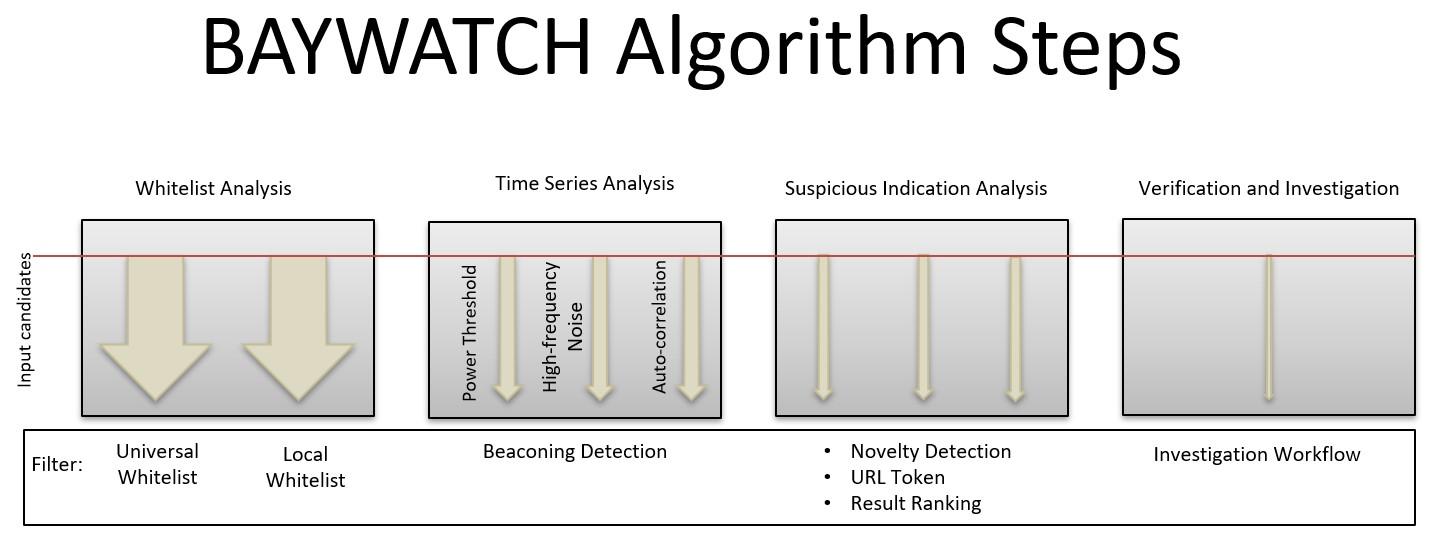
\includegraphics[width=\textwidth]{../Thesis_Docs/media/algorithm.jpg}
    \caption{Algorithm steps}
    \label{fig:steps}
\end{figure}

Figure \ref{fig:steps} provides a detailed overview of the algorithm's processing steps, which occur in four distinct phases. In Phase 1, the input data undergoes whitelist analysis, where it is categorized into two separate whitelists. The Universal Whitelist contains common, globally trusted URLs such as major search engines (e.g., Google, Yahoo) and other widely recognized platforms. The Local Whitelist, on the other hand, includes URLs that are specifically trusted within the organization, such as internal Allianz resolution URLs. This step helps to filter out trusted sources, ensuring that only potentially suspicious or unknown URLs are subjected to further analysis in subsequent phases.

Phase 2 focuses on time series analysis, where the algorithm processes the data to detect beaconing activity. Beaconing refers to the repeated communication of data to external servers, which can indicate malicious activity or unauthorized data exfiltration.

In Phase 3, the Suspicious Indication Analysis takes place. This phase is composed of several sub-processes aimed at identifying and ranking suspicious URLs. It includes Novelty Detection, which focuses on recognizing previously unseen or unusual patterns in the data; URL Token analysis, which breaks down and examines specific elements of URLs for signs of malicious intent; and Result Ranking, where URLs are ranked based on their likelihood of being malicious, helping to prioritize further investigation. This step refines the list of suspicious indicators to ensure that only the most relevant ones are brought forward for verification.

Finally, in Phase 4, the algorithm enters the Verification and Investigation phase. This is the concluding step where the flagged URLs and potential threats are thoroughly investigated and verified. This phase ensures that any suspicious activities are properly validated, confirming whether they are legitimate threats or false alarms. The outcome of this phase directly informs decision-making processes regarding the necessary actions to mitigate or resolve any identified risks.

\begin{figure}
    \centering
    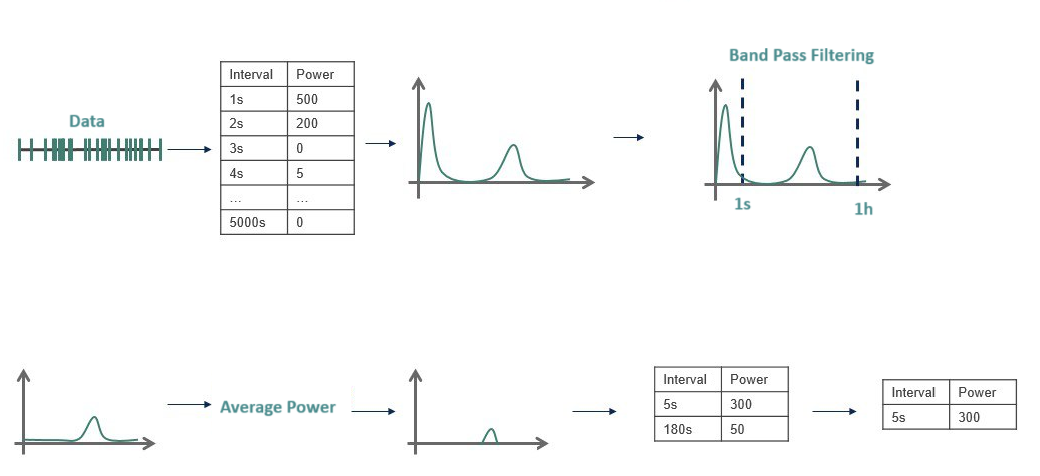
\includegraphics[width=\textwidth]{../Thesis_Docs/media/methodchart.png}
    \caption{Steps of the proposed method}
    \label{fig:mchart}
\end{figure}

Figure \ref{fig:mchart} visually represents the methodology for beaconing detection as proposed in thesis. The process begins with the collection of data, a first step that will be elaborated upon in detail later in the thesis. Following data collection, the methodology involves exact data cleaning and processing to ensure the accuracy and quality of the dataset. This stage addresses any inconsistencies or errors in the data, preparing it for more sophisticated analysis.

To enhance security and simplify data management for large organizations with diverse URL hostnames, a whitelist is implemented. This whitelist restricts user activity to domains containing "Allianz resolution." Also, common URLs such as major search engines and popular websites were added to the whitelist. By comparing this whitelist against all user data, entries associated with whitelisted domains are removed. This focused approach significantly reduces the volume of data to be processed, which is given that the dataset exceeds 500,000 entries per day. URLs included in the whitelist are deemed non-malicious and therefore do not require further behavior checks, streamlining the analysis.

Subsequently, the methodology calculates the time intervals for each domain and their occurrences within these intervals. This step is for identifying patterns and trends in beaconing activities, providing insight into the frequency and timing of these activities.

The next phase involves bandpass filtering to eliminate noise, retaining only the data within the time range of 1 second to 1 hour for further analysis. This filtering step focuses on relevant signals while minimizing interference from irrelevant data, ensuring that the analysis is both efficient and accurate.

Following filtering, the methodology includes the calculation of average power for each domain and subsequent normalization by adjusting all powers accordingly. In this context, the "power" metric indicates how frequently a particular website is visited within a given day. This metric relies on the assumption that each access to the website represents a distinct user interaction, with multiple accesses from the same user counted separately. The accuracy of the "power" measure depends on the consistency and reliability of the data collection methods used to track website visits. Domains exhibiting a negative decrease in power are disregarded, as they do not conform to expected patterns and are unlikely to be indicative of malicious activity.

Finally, the analysis phase involves a thorough examination of the data over time. Significant peaks observed during this analysis are indicative of potential malicious beaconing activity, marking the culmination of the beaconing detection process. This comprehensive methodology ensures that the detection system is robust, accurate, and capable of adapting to evolving threats, thereby enhancing the overall security and integrity of the network.
\section{Data Extraction and Preparation}
The dataset captures user activities as they navigate various URLs throughout the workday, including details such as the URLs visited, the date and time of each visit, and potentially other relevant information about user behavior or system interactions. This extensive data collection offers a detailed perspective on user activities and interactions, facilitating an in-depth analysis of browsing patterns and behaviors. Stored in a JSON file, the dataset benefits from JSON's flexibility and readability, making it easier to manage and manipulate large amounts of information. Each entry records a specific user interaction with precise time and date stamps, enabling a chronological reconstruction of user activities that is crucial for identifying patterns and trends over time, such as peak usage periods or frequent transitions between specific URLs. Overall, the dataset is a vital resource for analyzing user behavior, identifying significant patterns and trends, and supporting efficient data processing and analysis, which is  for developing effective beaconing detection strategies and enhancing overall network security.

Figure \ref{fig:jsondata} illustrates a sample JSON file entry, showcasing the detailed information captured for each user interaction. The entry includes  details such as the log date and time, the URL hostname visited, and potentially other relevant information about the user or system. This structured format ensures that each entry is consistent and comprehensive, providing a reliable record of user activities for analysis.

\begin{figure}
    \centering
    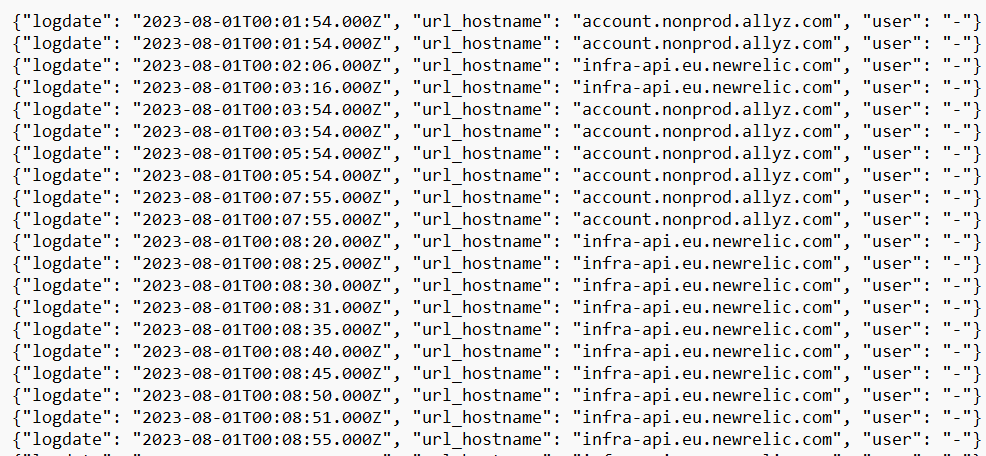
\includegraphics[width=.8\linewidth]{../Thesis_Docs/media/jsondata.png}
    \caption{Steps of the proposed method}
    \label{fig:jsondata}
\end{figure}

Each JSON file acts as a comprehensive record, including important information such as \texttt{"logdate"} (date and time) and \texttt{"url\_hostname"}.  The company prioritizes security; usernames are deliberately omitted during the import process for added protection. The following section outlines the Document Type Definition (DTD) for the JSON files.

\begin{lstlisting}[language=json]
{
  "$schema": "http://json-schema.org/draft-07/schema#",
  "type": "object",
  "properties": {
    "logdate": {
      "type": "string",
      "format": "date-time"
    },
    "url_hostname": {
      "type": "string"
    },
    "user": {
      "type": "string"
    }
  },
  "required": ["logdate", "url_hostname"]
}
\end{lstlisting}
The provided DTD serves as a specification for the structure and constraints of the dataset entries. It defines the expected format and mandatory fields for each log entry. Specifically:
\begin{itemize}
    \item \texttt{"logdate":} Specifies the date and time format for the log entry.
    \item \texttt{"url\_hostname":} Identifies the hostname of the accessed URLs.
    \item \texttt{"user":} Optional field denoting the user identifier.
\end{itemize}
This thesis proposes a sophisticated system for managing website connection data, designed to handle and analyze extensive logs of IP address connections to various domains. The system begins by utilizing InfluxDB, a highly specialized database optimized for managing time-series data. InfluxDB’s architecture is particularly well-suited for this application because it is engineered to efficiently handle high volumes of data with temporal components, such as timestamps associated with user interactions.

The data management methodology begins by importing the dataset into InfluxDB, initially focusing on a single day's data. This strategy ensures that the dataset remains manageable for initial processing, which is crucial for validating the system's functionality and performance before handling larger datasets. The dataset consists of JSON files that contain detailed logs of connections from various IP addresses to specific domains. These logs include timestamps, IP addresses, and domain names, providing a comprehensive record of user activity.

The success of this methodology depends on creating a well-structured data environment within InfluxDB. To achieve this, a predefined schema is implemented to dictate how the data is organized and stored within the database. This schema ensures data integrity and consistency by enforcing a uniform set of rules across all entries. Consistency in data structure is crucial as it facilitates smoother data processing and analysis, reducing the likelihood of errors and discrepancies.

Implementing this schema supports reliable data management by ensuring that each piece of information adheres to the same format and standards. This uniformity is for maintaining data quality, which in turn affects the reliability of subsequent analyses and research findings. Clean and reliable data is the cornerstone of trustworthy and effective research. Therefore, establishing a well-defined schema is a critical step in the proposed method. By prioritizing data integrity and consistency, the system lays a solid foundation for accurate and insightful analysis, ultimately contributing to the overall success of the proposed research methodology.

After establishing a well-structured data environment, the next step involves importing the data itself. This process follows a defined sequence, facilitated by custom Python scripts. These scripts automate the creation of a dedicated "bucket" within InfluxDB.

This method establishes a solid foundation for in-depth analysis by transforming raw, unstructured data into a well-organized format that is highly conducive to detailed examination. The strategic decision to import data for a specific day allows for a focused analysis of temporal patterns and variations, which are for uncovering trends and anomalies within a defined timeframe. This approach simplifies the analysis, making the data more manageable and representative of specific time-based behaviors. The JSON file structure, with its predefined key criteria and integrated security measures. It provides a clear and consistent framework for storing and accessing data, ensuring that each piece of information adheres to the same standards and is safeguarded against unauthorized access. This structured format supports efficient data processing and retrieval, which is vital for conducting thorough and accurate analyses of network interactions. By utilizing this organized data structure, the methodology enables a comprehensive exploration of user behavior, connection patterns, and potential security threats. This detailed examination is  for identifying vulnerabilities, detecting suspicious activities, and enhancing overall network security. The systematic approach not only facilitates a deeper understanding of the dataset but also sets the stage for generating actionable insights and implementing effective security measures.

The data is collected over the course of a single day, specifically a typical Tuesday workday, generating nearly 73 gigabytes of information. To derive meaningful insights from this data, it is to understand its behavior. Therefore, the initial step involved a thorough examination of the data's behavior. This analysis was conducted in several stages: observing the overall data behavior throughout the day, identifying the most frequently accessed or visited data sets and calculating their averages, analyzing the time intervals between each request, and examining the distribution of hosts. This approach provides a deeper understanding of usage patterns and helps identify any anomalies or trends present in the data. By analyzing the data's behavior, it is possible to gain valuable insights into user activity, resource utilization, and potential security risks, which are  for developing effective detection strategies and enhancing network security.

\subsection{Visualization of URL Request Counts}
To better understand the distribution and frequency of URL requests within the dataset, visual representations are utilized. These visualizations help in identifying patterns and anomalies in user behavior and resource utilization. The following figures provide insights into the request counts for different URLs, using both logarithmic and linear scales for comparison.

\begin{figure}
    \centering
    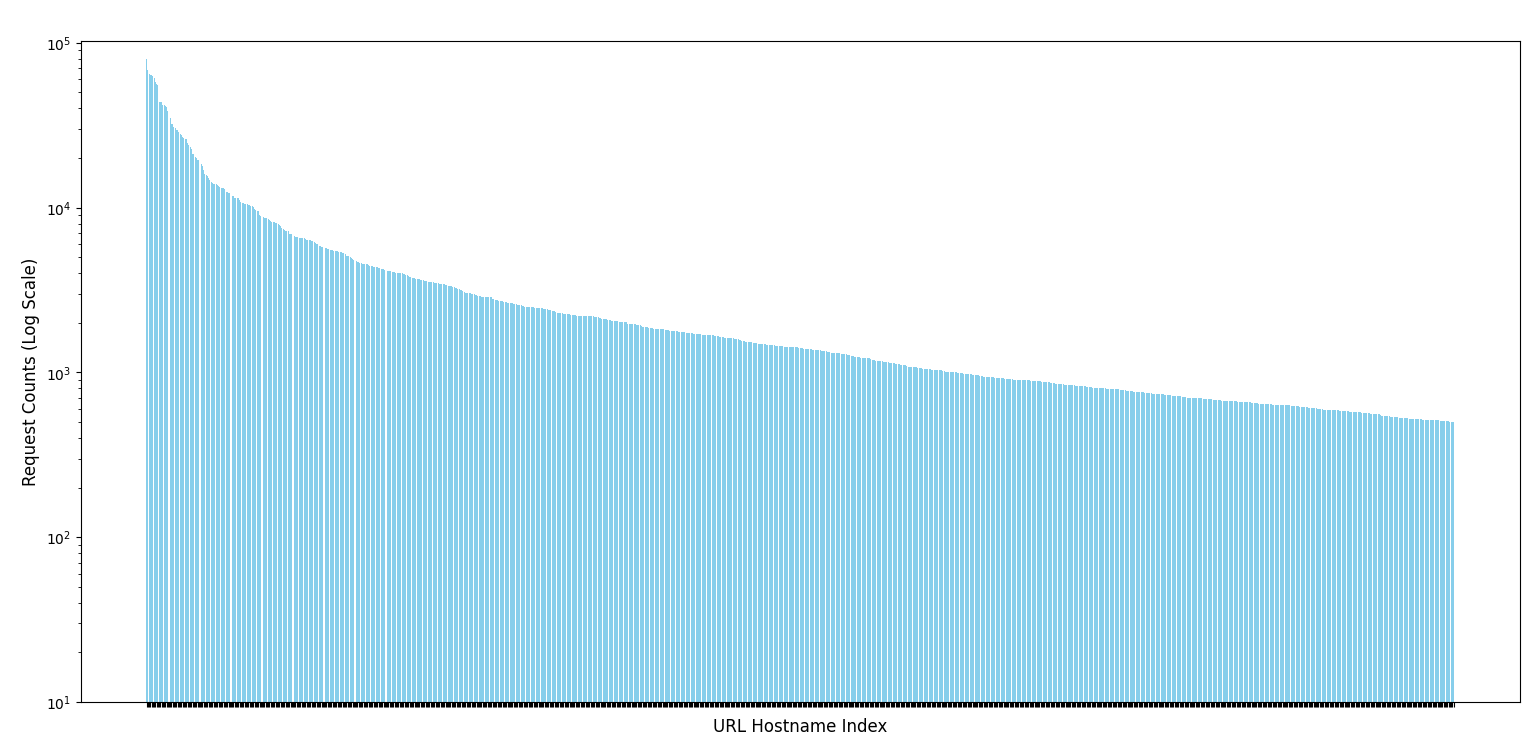
\includegraphics[width=\textwidth]{../Thesis_Docs/media/urls_request_count_log_scale.png}
    \caption{Request counts of URLs (log scale) }
    \label{fig:requestcount}
\end{figure}

Figure \ref{fig:requestcount} provides a visual representation of the request counts for different URLs within the dataset. The logarithmic scale on the Y-axis allows for a clearer comparison of the visit frequencies across URLs with varying levels of activity. This visualization highlights the distribution of request counts, showcasing the range of visit frequencies observed within the dataset. By examining this distribution, it is possible to identify URLs with high visit counts, which may indicate critical resources or frequently accessed services. Conversely, URLs with lower visit counts may represent less frequently accessed or less critical components of the network. This analysis provides valuable insights into user behavior and resource utilization, enabling organizations to optimize their network infrastructure and prioritize security measures effectively. 

\begin{figure}
    \centering
    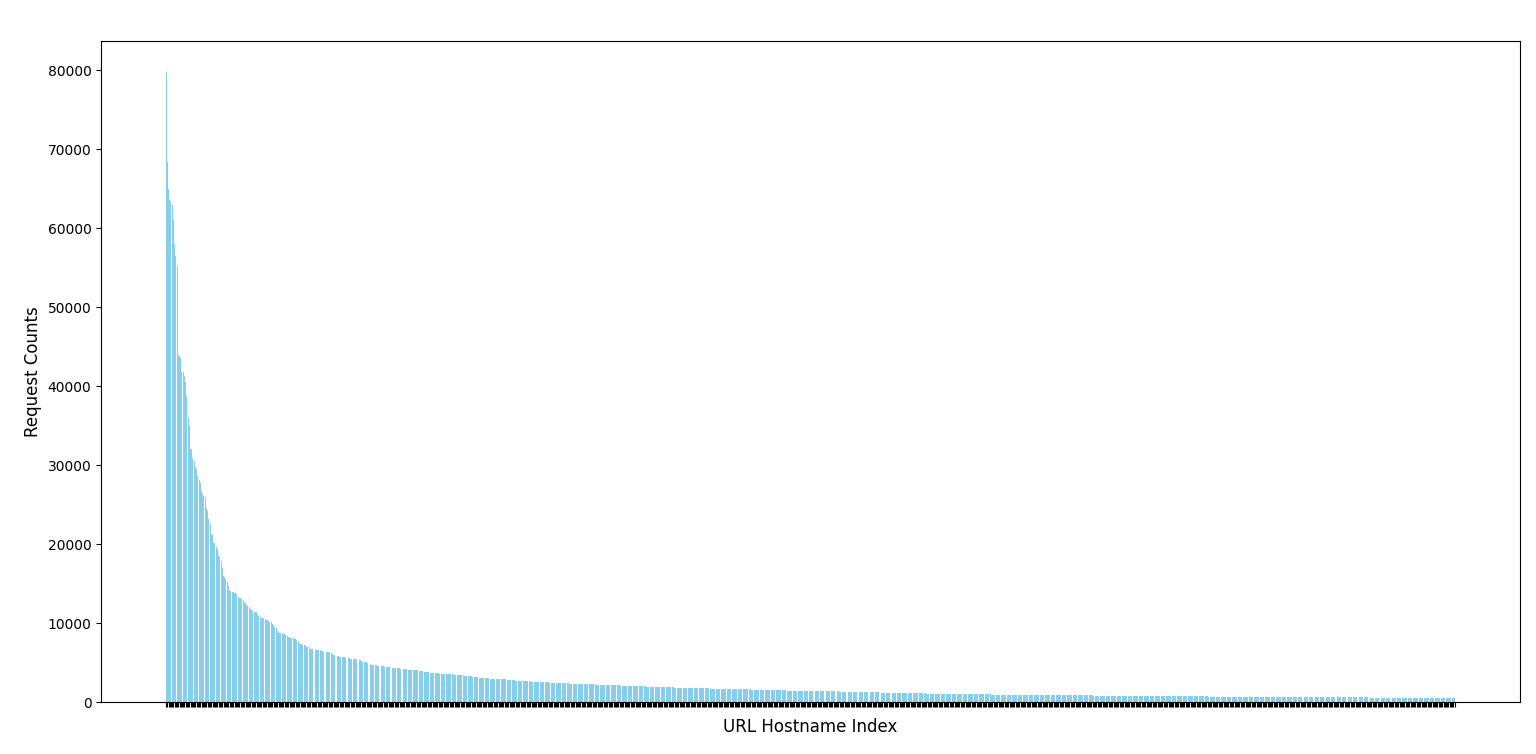
\includegraphics[width=\textwidth]{../Thesis_Docs/media/urls_request_count_linear_scale.png}
    \caption{Request counts of URLs (linear scale) }
    \label{fig:requestcountlinear}
\end{figure}

Figure \ref{fig:requestcountlinear} provides a linear scale representation of the request counts for different URLs within the dataset. This visualization offers a more detailed view of the visit frequencies across URLs, highlighting the distribution of request counts with greater granularity. By examining this distribution, it is possible to identify URLs with varying levels of activity, ranging from high-visit counts to low-visit counts. This analysis enables organizations to gain insights into user behavior and resource utilization, facilitating informed decision-making and strategic planning.

The logarithmic scale in Figure \ref{fig:requestcount} allows for a clearer comparison of URLs with varying request counts by compressing the scale for higher values and expanding it for lower values. This makes it easier to identify both high and low-frequency URLs, providing a balanced view of the data.

In contrast, the linear scale in Figure \ref{fig:requestcountlinear} presents the data with equal distances on the Y-axis representing equal differences in request counts. This offers a more detailed view of URLs with similar request counts but may obscure relative differences when the range of request counts is large. The choice between logarithmic and linear scales depends on the specific aspects of the data that need to be emphasized.

\subsection{24-Hour URL Visit Analysis}
To gain insights into the temporal patterns of URL visits, a 24-hour analysis is conducted. This analysis helps in understanding the distribution of user activity throughout the day, identifying peak usage times, and detecting periods of lower activity. Such temporal analysis is for recognizing trends and potential anomalies in user behavior.

\begin{figure}
    \centering
    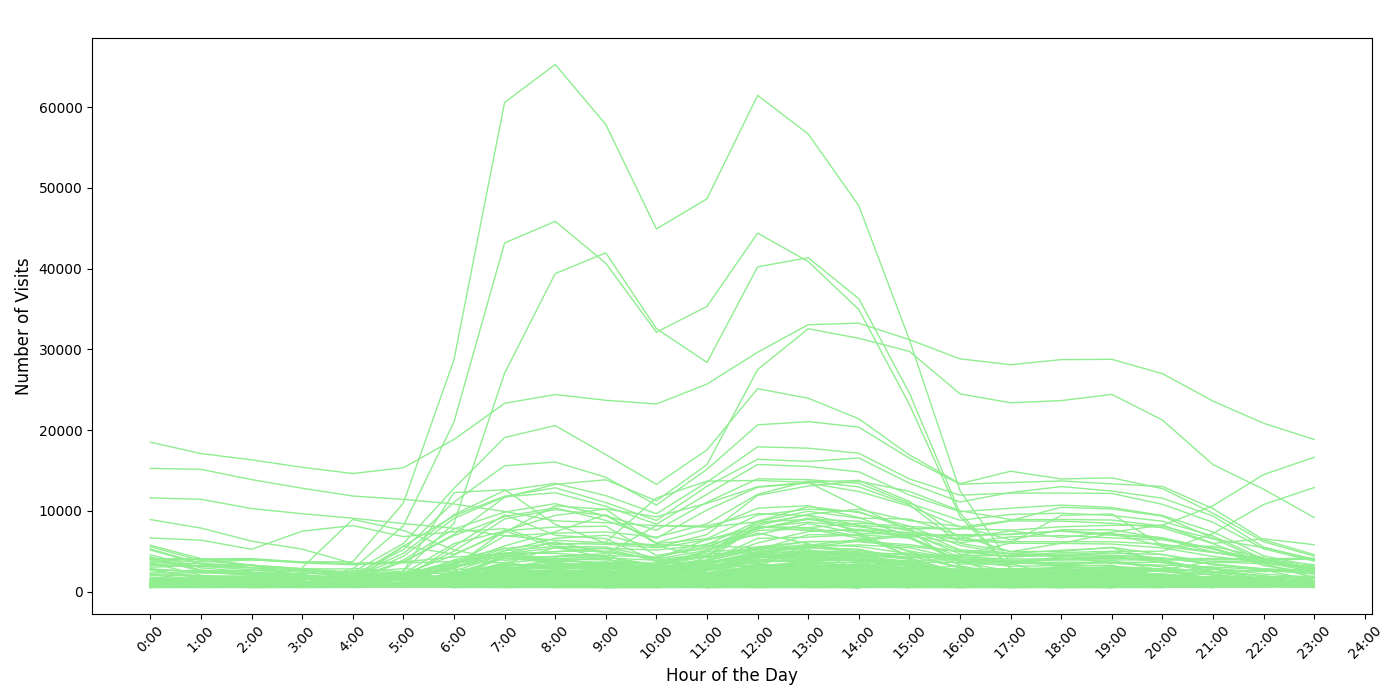
\includegraphics[width=\textwidth]{../Thesis_Docs/media/visit_in_24h.png}
    \caption{Number of visit by hour (24 hours)}
    \label{fig:24hvisit}
\end{figure}

Figure \ref{fig:24hvisit} illustrates the number of visits to different URLs over a 24-hour period. The x-axis represents the hours of the day, while the y-axis indicates the number of visits to each URL. This visualization provides a clear overview of the distribution of visits throughout the day, highlighting peak usage times and periods of lower activity. By examining this data, it is possible to identify trends and patterns in user behavior, which can be instrumental in detecting anomalies or suspicious activities. This analysis serves as a foundational step in understanding the dataset's behavior and establishing a baseline for further investigations.
As shown, the distribution of visits predominantly falls within the range of 0–500, which is significantly higher compared to the rest.

From the figure, it is evident that certain URLs exhibit high activity levels during the initial hours but experience a sharp decline, with their visit counts approaching zero around 04:00. This observation led to the categorization of URL activity into two distinct periods: day activity, which begins at 00:00 and ends at 04:00, and night activity, which spans from 04:00 to 24:00. To better understand these terms and analyze the patterns, the average number of visits during each period was calculated. This analysis provides valuable insights into how URL activity fluctuates throughout the day and highlights significant differences in usage between the two time frames, enabling more effective resource allocation and decision-making based on user behavior.

\begin{figure}
    \centering
    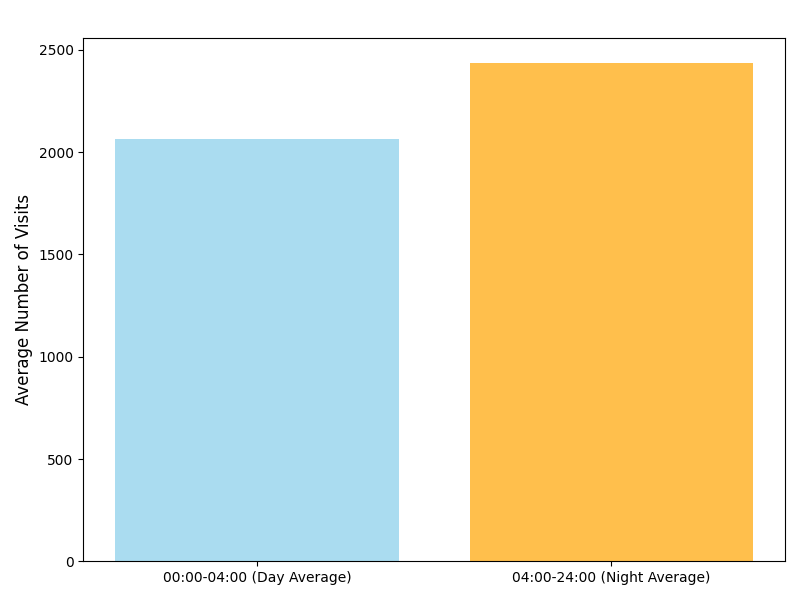
\includegraphics[width=\textwidth]{../Thesis_Docs/media/avg_day_night.png}
    \caption{Average number of visits during day and night}
    \label{fig:avg}
\end{figure}

Figure \ref{fig:avg} compares the average number of visits during two distinct time ranges: from 00:00 to 04:00 ("Day Average") and from 04:00 to 24:00 ("Night Average"). The "Day Average" is represented by a light blue bar, which shows an average number of visits slightly exceeding 2,000. On the other hand, the "Night Average" is depicted with an orange bar, which is taller and indicates a higher average of approximately 2,500 visits. The chart effectively highlights that the visitation rate is higher during the later time period, with the bars labeled clearly and a descriptive title ("Day vs. Night Average Visits") at the top. Additionally, the y-axis represents the average number of visits, ranging from 0 to 2,500, with consistent scaling and proper spacing for visual clarity. This analysis provides valuable insights into user behavior patterns and resource utilization, enabling organizations to optimize their network infrastructure and enhance security measures effectively.

\subsection{Time Interval Analysis of URL Requests}
To understand the temporal dynamics of user interactions, an analysis of the time intervals between requests for different URLs is conducted. This analysis helps in identifying patterns and trends in the timing of user activities, which can be crucial for optimizing network resources and enhancing security measures.

\begin{figure}
    \centering
    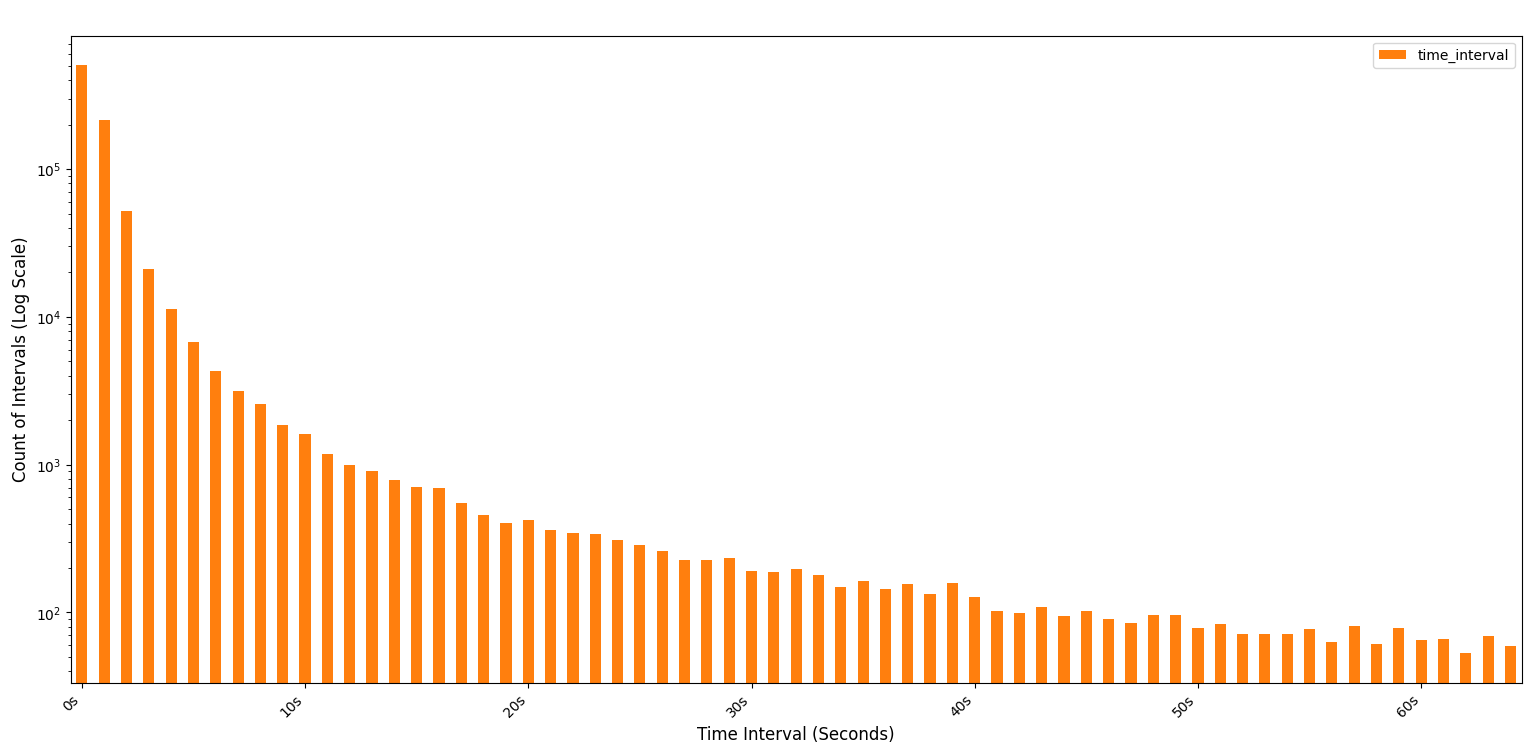
\includegraphics[width=\textwidth]{../Thesis_Docs/media/seconds.png}
    \caption{Time interval 0-65s (log scale) }
    \label{fig:timeintervallog}
\end{figure}

Figure \ref{fig:timeintervallog} illustrates the distribution of time intervals between requests for different URLs within the dataset. The logarithmic scale on the Y-axis allows for a clearer comparison of the time intervals across URLs with varying patterns of activity. The X-axis demonstrates the bins, which are divided into 90 bins. These bins are structured as follows: from 0 to 65 seconds, each second has its own bin. This visualization highlights the variability in time intervals between requests, showcasing the range of durations observed within the dataset. By examining this distribution, it is possible to identify URLs with distinct time interval patterns, which may indicate specific usage behaviors or interaction trends. This analysis provides valuable insights into the frequency and timing of user interactions, enabling organizations to optimize their network resources and enhance security measures effectively. As can be seen in the figure, the requests are decreasing across the entire time range, but every 10 seconds, the value is slightly higher than the previous second. This pattern is consistent across all URLs, indicating a common behavior in the dataset. This observation suggests that the time intervals between requests follow a specific pattern, which may be indicative of regular user activity or system behavior. By analyzing these patterns, organizations can gain valuable insights into user behavior and resource utilization, enabling them to optimize their network infrastructure and enhance security measures effectively. 

\begin{figure}
    \centering
    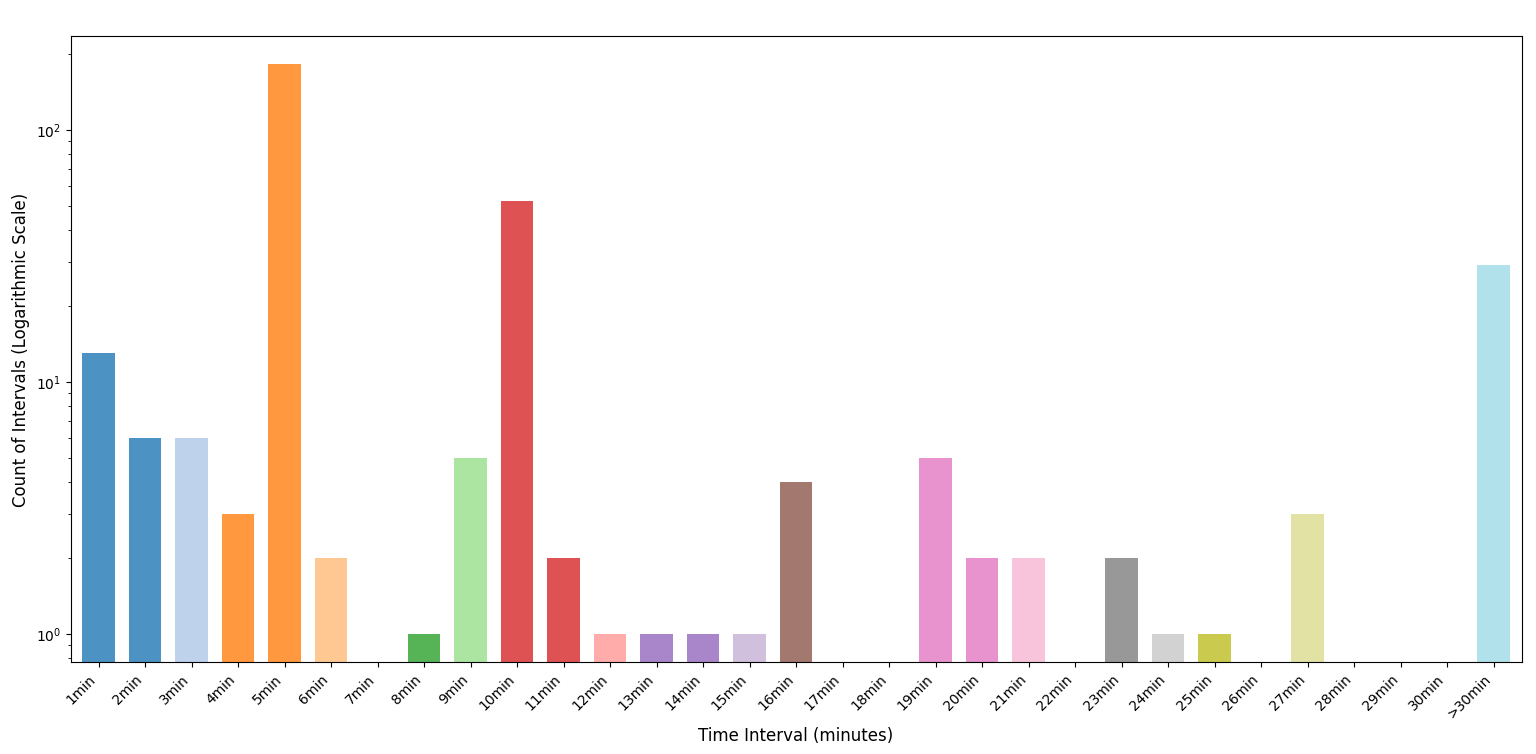
\includegraphics[width=\textwidth]{../Thesis_Docs/media/minutes.png}
    \caption{Time interval in minutes (log scale) }
    \label{fig:timeintervallogmin}
\end{figure}

Figure \ref{fig:timeintervallogmin} illustrates the distribution of time intervals between requests for different URLs within the dataset, with the Y-axis represented on a logarithmic scale. The X-axis demonstrates the bins, which are divided into 31 bins. These bins are structured as follows: Each bin shows the requests in minutes. To ensure that beaconing behavior at the edge of each minute is not missed, the number is shown with ±30 seconds. This visualization provides a detailed view of the time intervals between requests, highlighting the variability in durations observed within the dataset. By examining this distribution, it is possible to identify URLs with distinct time interval patterns, which may indicate specific usage behaviors or interaction trends. This analysis offers valuable insights into the frequency and timing of user interactions, enabling organizations to optimize their network resources and enhance security measures effectively. As can be seen in the figure, the requests are decreasing across the entire time range, but every minute, the value is slightly higher than the previous minute. This pattern is consistent across all URLs, indicating a common behavior in the dataset. This observation suggests that the time intervals between requests follow a specific pattern, which may be indicative of regular user activity or system behavior. By analyzing these patterns, organizations can gain valuable insights into user behavior and resource utilization, enabling them to optimize their network infrastructure and enhance security measures effectively.

both figures \ref{fig:timeintervallog} and \ref{fig:timeintervallogmin} provide a detailed view of the time intervals between requests for different URLs within the dataset. The logarithmic scale on the Y-axis allows for a clearer comparison of the time intervals across URLs with varying patterns of activity. The scale is in logarithmic because, in the linear scale, the differences in time intervals were not shown as clearly. The differences between the bins were too large. The X-axis demonstrates the bins, which are divided into 90 bins for seconds and 31 bins for minutes. These bins are structured to capture the variability in time intervals between requests, showcasing the range of durations observed within the dataset. By examining this distribution, it is possible to identify URLs with distinct time interval patterns, which may indicate specific usage behaviors or interaction trends. This analysis provides valuable insights into the frequency and timing of user interactions, enabling organizations to optimize their network resources and enhance security measures effectively. The consistent patterns observed in the time intervals between requests suggest a regularity in user behavior or system interactions, which may be indicative of normal network activity. By analyzing these patterns, organizations can gain valuable insights into user behavior and resource utilization, enabling them to optimize their network infrastructure and enhance security measures effectively.

\subsection{Distribution of Hosts Based on Unique URLs Contacted}
To analyze the interaction patterns of hosts within the network, a bar chart is used to illustrate the distribution of hosts (IP addresses) based on the number of unique URLs they contacted. This analysis helps in understanding the concentration of network activity and identifying key services or domains being accessed.

\begin{figure}
    \centering
    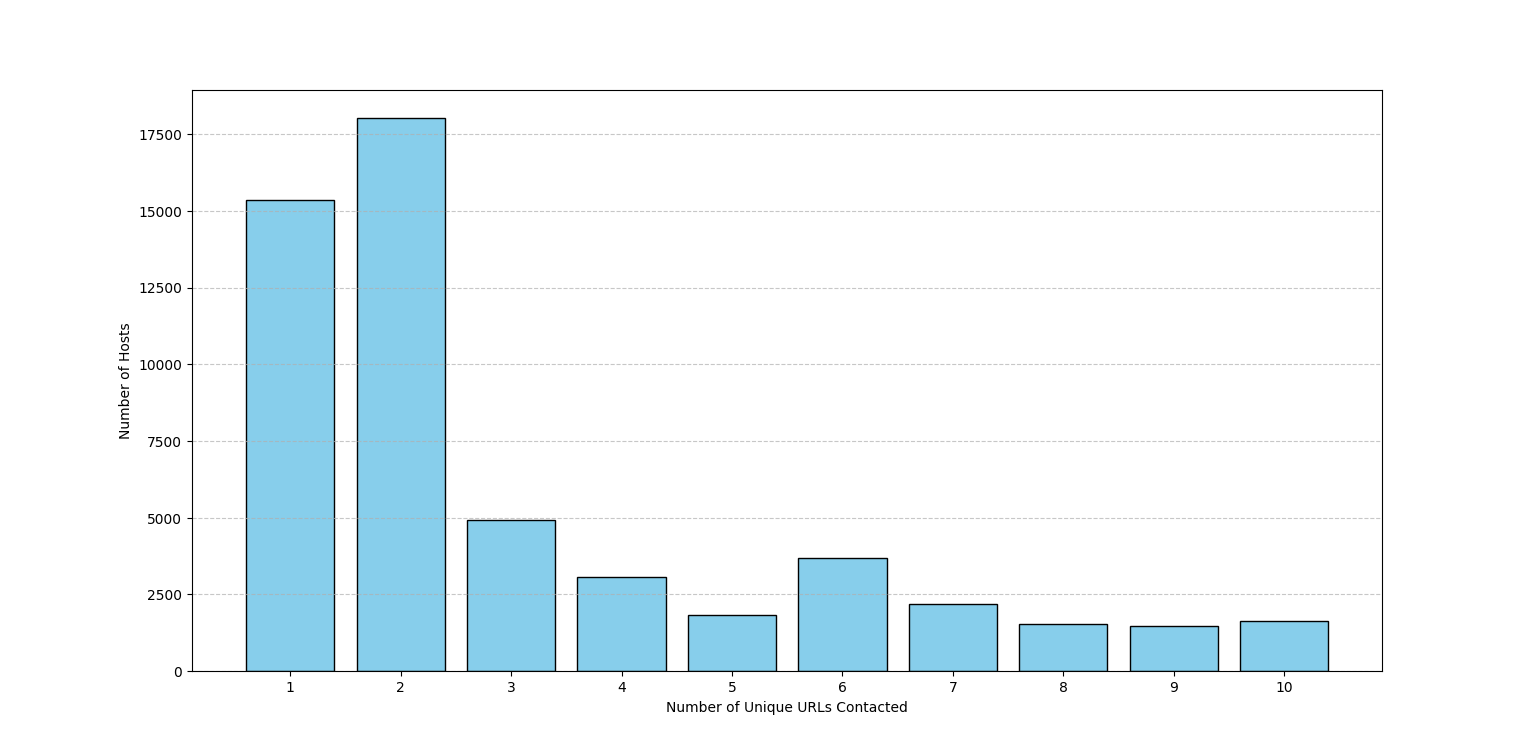
\includegraphics[width=\textwidth]{../Thesis_Docs/media/unic_urls.png}
    \caption{Distribution of hosts }
    \label{fig:ip}
\end{figure}

Figure \ref{fig:ip} The bar chart provides an analysis of the distribution of hosts (IP addresses) based on the number of unique URLs they contacted. The X-axis represents the number of unique URLs contacted by each host, ranging from 1 to 10, while the Y-axis depicts the total count of hosts for each corresponding category. Each bar in the chart indicates how many hosts interacted with a specific number of unique URLs. The data reveals a clear trend: the majority of hosts engaged with only a small number of unique URLs. Specifically, the highest number of hosts, approximately 17,500, connected to exactly two unique URLs. This is followed closely by the category of hosts that connected to only one unique URL, which includes around 15,000 hosts. As the number of unique URLs increases beyond two, there is a steady decline in the number of hosts. For instance, significantly fewer hosts contacted 4 or more unique URLs, and the numbers continue to diminish as the variety of URLs increases. This pattern suggests that most network activity is concentrated on a limited set of destinations, with relatively few hosts interacting with a wide range of URLs. Such insights could be valuable for understanding traffic patterns, identifying key services or domains being accessed, and optimizing network performance or security measures. The visualization highlights the sparsity of hosts interacting with a larger variety of destinations, emphasizing the importance of focusing on the most commonly accessed URLs in any further analysis or intervention.

\section{Data Preprocessing}
The initial step in the data cleaning process involves separating all URL hostnames from one another. Once these hostnames are isolated, they are systematically sorted by date. This sorting step serves several important purposes. Firstly, it organizes the data chronologically, which facilitates the identification of trends or patterns that emerge over time. For instance, if there is a need to investigate a specific security incident that occurred on a certain day, sorting the data by date allows for a more focused and efficient search, thereby reducing the time and effort required to locate the relevant information. Secondly, sorting by date prepares the data for subsequent stages in the data management workflow. Many data analysis techniques depend on the data being arranged in a specific sequence, and organizing the data chronologically ensures that it is ready for these advanced analytical processes. This stage of the cleaning process effectively transforms raw data into a structured and coherent format, which is necessary for performing in-depth analyses of network interactions and identifying potential security threats. Additionally, this preprocessing step includes the creation of a whitelist from all URL hostnames. Since the company frequently accesses a variety of trusted URLs multiple times throughout the day, establishing a whitelist helps to streamline the algorithm’s operations. By compiling a list of these consistently trusted URLs, the algorithm's efficiency is enhanced, allowing it to operate more quickly and effectively. This improved efficiency supports the algorithm's ability to detect potentially suspicious activities within network interactions more accurately. Through this cleaning process, raw data is organized into a format that is both structured and easily analyzable, setting the stage for comprehensive insights into network behaviors and security risks.

\begin{figure}
    \centering
    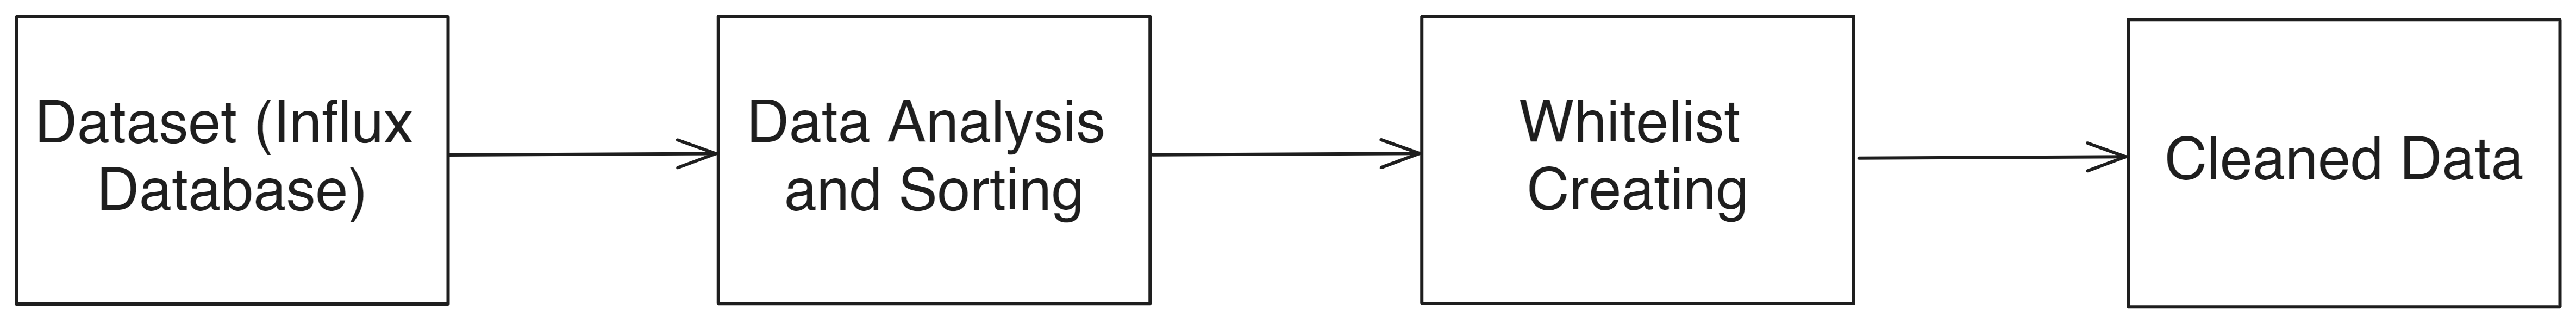
\includegraphics[width=\textwidth]{../Thesis_Docs/media/datasetchart.png}
    \caption{Dataset}
    \label{fig:datasetchart}
\end{figure}

In Figure \ref{fig:datasetchart}, the various steps undertaken to process the data are illustrated, beginning with the initial stages of data collection and extending through to the final preparation required before the algorithmic process can commence. This visual representation outlines how the raw data is first gathered and then cleaned to ensure accuracy and consistency. The process includes several key stages, each designed to transform the raw, unprocessed data into a well-organized dataset that is ready for detailed algorithmic examination.

The initial stage involves data collection, where raw data is gathered from various sources such as network logs, user activity records, and system monitoring tools. This data is often unstructured and contains noise, making it necessary to undergo a thorough cleaning process. The first step in cleaning involves separating all URL hostnames from the collected data. This separation is crucial for isolating relevant information and discarding any extraneous data that may interfere with the analysis.

Once the URL hostnames are isolated, they are sorted by date. Chronological sorting is for identifying trends and patterns over time, which can be particularly useful for investigating specific security incidents. By organizing the data by date, it becomes easier to focus on relevant time periods and reduce the time and effort required to locate pertinent information. This step also prepares the data for subsequent stages in the data management workflow, ensuring that it is in the correct sequence for advanced analytical techniques.

Following the sorting process, a whitelist of frequently accessed, trusted URLs is created. This whitelist helps streamline the algorithm's operations by allowing it to bypass known, safe URLs and focus on potentially suspicious activities. By enhancing the algorithm's efficiency, this step ensures quicker and more accurate detection of anomalies within the network interactions. The creation of a whitelist is particularly important for organizations that frequently access a variety of trusted URLs, as it helps to reduce false positives and improve the overall performance of the analysis.

The cleaned and organized data is then prepared for advanced analytical techniques. This preparation involves structuring the data in a format suitable for algorithmic processing, ensuring that it is ready for in-depth analysis. The final dataset is well-organized, consistent, and free of noise, making it ideal for detailed examination and the extraction of valuable insights. This stage of the process is crucial for transforming raw data into a structured and coherent format, which is necessary for performing in-depth analyses of network interactions and identifying potential security threats.

By following this structured approach, the methodology ensures that the data is prepared effectively for analysis, enhancing the accuracy and reliability of the results obtained. This systematic process of data preparation is for generating meaningful insights and actionable outcomes from the dataset, ultimately contributing to the success of the research methodology. The visual representation in Figure \ref{fig:datasetchart} highlights the importance of each step in the data processing workflow, emphasizing the need for a thorough and methodical approach to data preparation. Through this process, raw data is transformed into a valuable resource that can be used to gain comprehensive insights into network behaviors and security risks, enabling organizations to optimize their network infrastructure and enhance their security measures effectively.

\section{Data Enhancement}
In the context of this analysis, "power" is defined as a metric representing the frequency of visits to each unique website within the dataset. Once the "power" for all URLs in the dataset is calculated, representing the frequency of visits to each unique website, the next step involves computing the average power. The "power" metric serves as a quantitative measure of how often each website is accessed within a given timeframe, providing valuable insight into user behavior patterns. The average power acts as a reference point or baseline against which the individual powers are compared, allowing for the identification of significant deviations from typical visit frequencies. To determine the average power, the total power across all URLs is summed and then divided by the number of URLs in the dataset. This average power serves as a benchmark, providing a context for evaluating the frequency of visits to each specific URL. By establishing this baseline, the methodology can differentiate between normal and abnormal activity levels, thereby facilitating the identification of URLs that exhibit unusual patterns of access. 

After determining the average power, each calculated power is assessed relative to this baseline. The evaluation process involves comparing the power of each URL to the average power to identify significant deviations. Specifically, the power of each URL is subtracted from the average power. If the resulting value is negative, indicating that the URL's visit frequency is below the baseline, it is omitted from further analysis. This step ensures that the focus remains on URLs with visit frequencies that significantly exceed the norm, which are more likely to represent meaningful patterns or anomalies. The rationale behind omitting negative deviations is based on the premise that these values do not provide meaningful insights into unusual behavior or potential security threats. By filtering out these less significant data points, the methodology enhances the quality and relevance of the dataset. This focused approach allows for a more efficient examination of the data, concentrating on positive deviations that indicate higher-than-average visit frequencies. 

Focusing on significant deviations from the average power refines the dataset, making it more manageable and pertinent for further analysis. This step not only improves the efficiency of the data processing but also enhances the ability to detect anomalies that could signify security threats or other irregularities. By concentrating on URLs with visit frequencies that stand out from the baseline, the methodology increases the likelihood of identifying genuinely noteworthy patterns. In summary, the calculation of average power and the subsequent evaluation of individual powers against this baseline are critical components of the data enhancement process. By omitting powers that result in negative values, the methodology ensures that the dataset is refined to include only significant deviations. This targeted focus on relevant patterns and anomalies lays the groundwork for a more detailed and accurate analysis of network interactions and potential threats, ultimately contributing to a more robust and reliable security framework.

\section{Band-Pass Filtering}
In network processing, bandpass filtering is a technique employed to dissect time-series data, allowing the extraction of specific frequency components within a predefined range. This technique is particularly useful in analyzing patterns in HTTP requests. Bandpass filtering involves the application of a filter that selectively passes signals whose frequencies fall within a certain range, known as the "bandpass" range. By isolating these specific frequencies, the technique enables a focused examination of data that is most relevant to the analysis, effectively filtering out noise and irrelevant information. This selective process enhances the clarity and precision of the data, making it easier to identify significant patterns and trends in HTTP requests. For instance, in a dataset containing web traffic data, bandpass filtering can help highlight the intervals and frequencies at which certain URLs are accessed, providing insights into user behavior and potential security threats. The ability to concentrate on a specific frequency range allows analysts to zero in on the most pertinent signals, thereby improving the accuracy and effectiveness of the analysis.

Furthermore, bandpass filtering aids in detecting anomalies and irregularities within the network. By focusing on the relevant frequency components, it becomes easier to spot deviations from the norm, which could indicate unusual or suspicious activity. This method is instrumental in the context of network security, where identifying and understanding these anomalies is key for protecting against potential threats. In addition to its application in security, bandpass filtering is also valuable for optimizing network performance. By understanding the regular patterns of data flow and identifying any irregular spikes or drops, network administrators can make informed decisions to enhance the efficiency and reliability of the network. This comprehensive approach ensures that only the most significant data is analyzed, leading to more accurate and actionable insights. Overall, bandpass filtering is a powerful technique in-network processing, enabling the extraction of meaningful information from large datasets. By focusing on specific frequency components, it facilitates a detailed and precise analysis of network interactions, helping to uncover important patterns and trends. This technique not only improves the understanding of user behavior and network performance but also plays a vital role in enhancing security by detecting potential threats and anomalies.

The bandpass filter formula can be expressed as:

\[ H(\omega) = \frac{1}{1 + \frac{\mathrm{j}(\omega - \omega_{\text{low}})}{\omega_{c}}} \cdot \frac{1}{1 + \frac{\mathrm{j}(\omega_{\text{high}} - \omega)}{\omega_{c}}} \]

Where:
\begin{itemize}
    \item \( H(\omega) \) is the frequency response of the bandpass filter,
    \item \( \omega \) is the angular frequency,
    \item \( \omega_{\text{low}} \) is the low cut-off frequency,
    \item \( \omega_{\text{high}} \) is the high cut-off frequency,
    \item \( \omega_{c} \) is the critical frequency.
  \end{itemize}

The bandpass filter selectively passes frequencies between the low cut-off frequency (\(\omega_{\text{low}}\)) and the high cut-off frequency (\(\omega_{\text{high}}\)), while attenuating frequencies outside this range. This formula provides a mathematical representation of how the bandpass filter operates to isolate specific frequency components within the defined range.

\section{Creation of Artificial Data}
To study and analyze beaconing behavior, artificial data was meticulously crafted to replicate typical network traffic intervals. The primary objective of this data generation process was to create a controlled yet realistic scenario that mimicked frequent "beacons" (network requests). These beacons were designed to occur at either regular or irregular time intervals, simulating both periodic and non-periodic network traffic patterns. A crucial aspect of this data was ensuring that each interval contained more than 1000 network requests, a condition that helps to highlight patterns and periodicity more effectively.

The artificial dataset was generated by assigning timestamps to events such that certain intervals exhibited regular, fixed time gaps, while others were assigned randomly varying time gaps to simulate randomness. This mix of regularity and randomness allowed the dataset to emulate real-world network conditions, where periodic beaconing can often be masked by non-periodic noise or deviations. The intervals were computed as the differences between consecutive timestamps, enabling precise time-series analysis.

The generated data was stored in an InfluxDB time-series database for efficient querying and processing. The database format facilitated the seamless retrieval of data for subsequent analytical methods, such as Fast Fourier Transform (FFT) and autocorrelation. The artificial dataset served as an  foundation for evaluating the robustness of algorithms in detecting periodic patterns in network traffic.

\section{Fast Fourier Transform (FFT) Function}
The Fast Fourier Transform (FFT) is a computational technique designed to analyze signals by transforming time-domain data into the frequency domain. This transformation provides insights into the periodic components of the data, which are otherwise challenging to identify in the time domain.

In this analysis, the FFT function was applied to the intervals between beaconing events. The input to the FFT was the sequence of interval durations, representing the time differences between consecutive network requests. The output consisted of two critical components: frequency bins and corresponding amplitudes. Each frequency bin represented a specific frequency component within the data, while the amplitude indicated the strength or magnitude of that frequency.

Peaks in the amplitude spectrum were interpreted as dominant periodic components, revealing the frequencies at which beaconing behavior occurred most strongly. For example, a sharp peak at a particular frequency indicated a high degree of periodicity at that frequency, suggesting that network requests occurred regularly at the corresponding interval. In contrast, the absence of distinct peaks indicated either non-periodic behavior or broadband noise in the signal.

The FFT results were visualized in a frequency-amplitude plot, which provided a clear depiction of the frequency components of the data. This visualization highlighted the periodic nature of certain intervals, offering a quantitative basis for detecting and analyzing beaconing behavior. Additionally, the ability to discern narrowband (sharp peaks) versus broadband (distributed peaks) characteristics further enriched the understanding of the network traffic patterns.

\begin{figure}
    \centering
    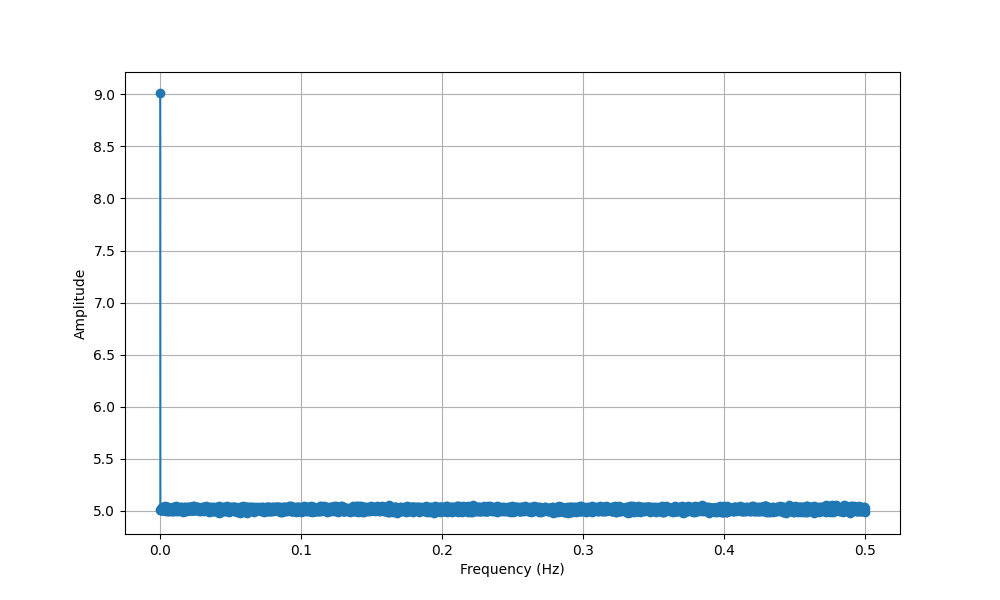
\includegraphics[width=\textwidth]{../Thesis_Docs/media/FTT Analysis.png}
    \caption{FFT Analysis of Beaconing Intervals}
    \label{fig:FastFourierTransform}
\end{figure}

Figure \ref{fig:FastFourierTransform} illustrates the results of the FFT analysis applied to the intervals between beaconing events. The x-axis represents the frequency bins, while the y-axis indicates the corresponding amplitudes. Peaks in the amplitude spectrum are highlighted, indicating the presence of dominant frequency components within the data. The sharp peak at a specific frequency signifies a strong periodic signal, suggesting that beaconing events occurred regularly at that interval. In contrast, a lack of distinct peaks or a broad distribution of amplitudes indicates randomness or noise in the signal. This analysis provides valuable insights into the periodicity of network traffic patterns, enabling the detection of beaconing behavior and other recurring activities. By leveraging the FFT function, organizations can gain a deeper understanding of their network traffic and identify potential security threats more effectively.

\section{Autocorrelation Function}
Autocorrelation is a statistical technique used to measure the degree of similarity between a signal and its lagged versions over time. It is particularly useful for identifying periodicity and repeating patterns within a dataset.

In this study, the autocorrelation function was applied to the intervals between beaconing events to examine how the intervals related to one another at varying time lags. The analysis involved computing the correlation of the interval sequence with itself, shifting the sequence by one step at a time (lag) and recalculating the correlation at each step. The resulting autocorrelation values quantified the degree of alignment or similarity between the original and lagged sequences.

The autocorrelation plot displayed the values for each lag, with the highest value occurring at lag 0 (self-correlation). Peaks at specific positive lags indicated recurring patterns, where intervals repeated with a certain periodicity. For instance, a peak at lag \(k\) suggested that the intervals separated by \(k\) steps were highly similar, signaling periodic behavior.

The decay of autocorrelation values as the lag increased provided additional insights into the data. A gradual decay indicated the presence of long-range dependencies, while a rapid decay suggested randomness or a lack of periodic structure. This function proved instrumental in distinguishing between regular and irregular patterns in the dataset, shedding light on the underlying structure of the simulated beaconing behavior.

The combined use of FFT and autocorrelation provided complementary perspectives on the periodicity and randomness of the intervals, enabling a robust analysis of the artificial data.

\begin{figure}
    \centering
    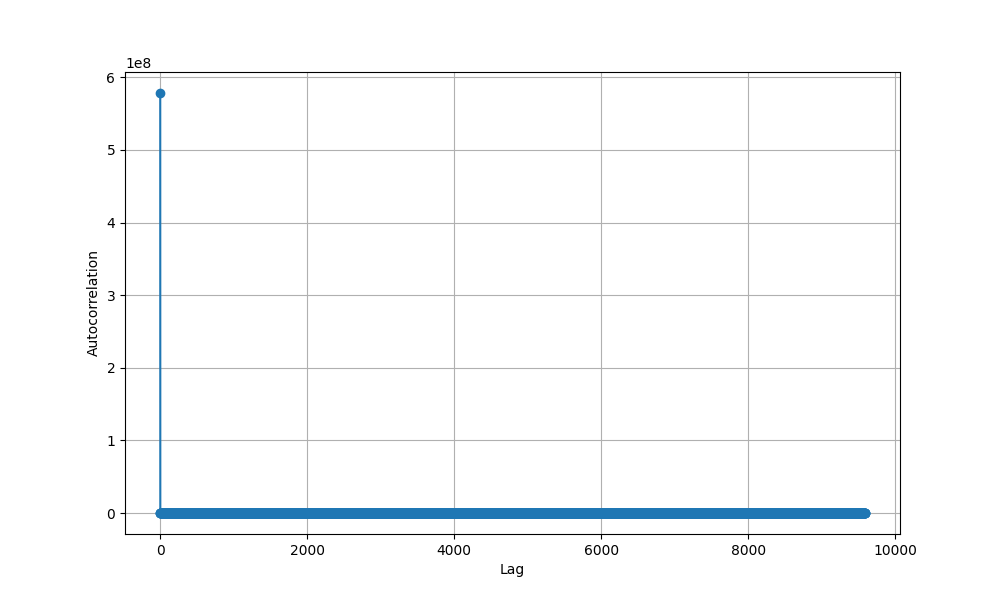
\includegraphics[width=\textwidth]{../Thesis_Docs/media/autocorrelation.png}
    \caption{Autocorrelation Analysis of Beaconing Intervals}
    \label{fig:Autocorrelation}
\end{figure}

Figure \ref{fig:Autocorrelation} depicts the results of the autocorrelation analysis applied to the intervals between beaconing events. The x-axis represents the lag values, while the y-axis indicates the autocorrelation values. Peaks in the autocorrelation plot correspond to recurring patterns in the data, with higher values indicating stronger correlations between intervals at specific lags. The presence of distinct peaks at positive lags signifies periodic behavior, where intervals repeat with a certain frequency. The decay of autocorrelation values as the lag increases provides insights into the temporal dependencies and structure of the data. A gradual decay suggests long-range dependencies, while a rapid decay indicates randomness or lack of periodicity. This analysis offers valuable insights into the underlying patterns of network traffic, enabling the detection of beaconing behavior and other recurring activities. By leveraging the autocorrelation function, organizations can gain a deeper understanding of their network interactions and identify potential security threats more effectively.

\section{Evaluation Criteria}
The Python-based data evaluation process uncovers instances of beaconing behavior within the dataset, offering valuable insights for experts to identify potential malicious activities. This task goes beyond merely visualizing the algorithm's output; it heavily depends on the expertise of professionals who sift through vast amounts of data to detect subtle signs of malicious behavior. The evaluation involves analyzing user behavior patterns to spot any anomalies or suspicious activities indicative of beaconing. Beaconing, a technique used by malicious actors, involves repetitive signal transmissions that enable compromised systems to communicate with external servers. Detecting such behavior requires advanced analysis techniques and a deep understanding of network traffic patterns.

Utilizing Python's powerful data analysis and processing capabilities, the evaluation process starts with the systematic analysis of large volumes of network data. Python's libraries and tools facilitate the handling and manipulation of complex datasets, aiding in the detection of beaconing signals embedded within regular network traffic. The process involves applying various algorithms and analytical methods to sift through the data, identifying patterns that deviate from normal user behavior. This initial algorithmic analysis provides a foundation, but the true strength of the evaluation lies in the subsequent expert review.

Experts play a crucial role in this process, as they interpret the algorithmic findings within the broader context of network activity. They scrutinize the identified patterns, cross-referencing them with known threat indicators and leveraging their experience to assess the likelihood of malicious intent. This human expertise is essential for distinguishing between benign anomalies and genuine threats. Upon detecting suspicious behavior, experts are tasked with making informed decisions on how to address the implicated users and domains. This involves a risk assessment to determine the severity and potential impact of the detected activity.

Decisions on handling identified threats may include a range of actions, from closely monitoring the suspect activity to implementing immediate mitigation measures such as blocking the suspicious domains or isolating affected systems. The evaluation process also involves documenting the findings and actions taken, ensuring a comprehensive record that can be used for future reference and continuous improvement of the detection system.

The integration of Python's technical capabilities with the nuanced understanding of skilled analysts results in a robust and dynamic approach to network security. This comprehensive approach not only enhances the accuracy of detecting beaconing behavior but also ensures that potential threats are thoroughly understood and effectively mitigated. By combining automated data processing with expert analysis, the methodology provides a reliable framework for maintaining network security and proactively addressing emerging threats. The continuous evaluation and refinement of this process are vital for staying ahead of increasingly sophisticated cyber threats, ultimately safeguarding the integrity and security of network environments.
\chapter{Implementation}
This chapter introduces the implementation of the proposed methodology within Allianz Company's network infrastructure, delving into the intricate process of adapting the system to integrate seamlessly with the company's extensive log data. It begins by exploring the necessary adjustments made to align the methodology with Allianz's specific log data formats and structures, highlighting the critical decisions in parameter selection and the strategic use of various analytical tools. The chapter aims to provide a comprehensive evaluation of the performance metrics derived from this implementation, offering a detailed analysis of the methodology's efficacy. Supported by visualizations such as graphs and charts, this analysis facilitates a clearer understanding of complex data and key findings.

Furthermore, the chapter rigorously assesses the methodology's effectiveness in detecting malicious behavior, providing an in-depth examination of detected anomalies, their correlation with potential security threats, and the system's responsiveness. This assessment underscores the practical value of the methodology, demonstrating its significant impact on enhancing network security. By presenting concrete evidence of the methodology's success in identifying and mitigating threats, the chapter establishes a foundation for discussing advanced security strategies.

The insights gained from this implementation are important for Allianz, as they pave the way for continuous improvement initiatives and the development of more robust security measures. This chapter sets the stage for broader discussions on enhancing network security, offering a clear pathway for future chapters to explore advanced techniques and strategies aimed at fortifying Allianz's network infrastructure against the ever-evolving landscape of cyber threats. Through this comprehensive examination, the chapter not only highlights the immediate benefits of the methodology but also its long-term potential to significantly bolster Allianz's cybersecurity framework.

\section{Experimental Setup}
This section details the adaptation process to integrate the methodology within Allianz Company’s network infrastructure. Initially, adjustments were made to ensure compatibility with the company’s log data, involving comprehensive data mapping and transformation to align with the methodology's requirements. This step was key to guarantee that the raw data could be accurately interpreted and utilized by the detection algorithms. Stringent measures were taken to address any discrepancies or inconsistencies encountered during the integration process. These measures included validating data integrity, standardizing log formats, and resolving any anomalies to ensure seamless integration.

For testing purposes, an experimental framework was established. This framework was designed to cover a wide range of scenarios, from routine network operations to sophisticated simulated cyber-attacks. These scenarios were crafted to assess the methodology's performance under diverse conditions, providing a realistic and thorough evaluation. The scenarios mimicked real-world network behaviors, encompassing various types of user activities, network loads, and potential threat vectors. This comprehensive testing ensured that the methodology was robust and applicable in practical settings, capable of handling the dynamic nature of real-world network environments.

Additionally, real data sourced from Allianz Company was utilized to validate the methodology's efficacy under authentic operational conditions. This real-world validation was a critical component of the adaptation process, as it provided invaluable insights into the methodology's performance in a live environment. The use of genuine operational data bolstered the credibility and relevance of the methodology, demonstrating its practical utility in addressing real-world cybersecurity challenges. By evaluating the methodology against actual network traffic and user behavior, the team could identify and address any limitations, fine-tuning the system to enhance its effectiveness.

Throughout the testing phase, data collection was conducted rigorously, capturing a comprehensive array of network activities and events. This extensive data collection ensured a rich dataset for analysis, encompassing a wide variety of normal and abnormal behaviors. The collected data served as the foundation for subsequent analyses, enabling a thorough and detailed evaluation of the methodology's effectiveness in detecting and mitigating malicious behavior within Allianz Company’s network infrastructure. The analysis focused on identifying patterns and anomalies indicative of malicious activity and assessing the accuracy and reliability of the detection algorithms.

The comprehensive approach to adaptation and testing detailed in this section underscores the methodology's readiness for real-world deployment. By ensuring data compatibility, rigorously testing under diverse scenarios, and validating with real-world data, the methodology is demonstrated to be not only theoretically sound but also practically effective. This robust process lays a solid foundation for enhancing Allianz's network security, providing a reliable tool to tackle the complex cybersecurity issues faced by the organization. The insights and results garnered from this extensive testing phase set the stage for further refinement and optimization, ensuring that the methodology remains effective against evolving cyber threats.

\section{Whitelisting Mechanism for URL Filtering}
In the heart of Allianz Company’s expansive network infrastructure, a pivotal decision was made to bolster its security framework: the establishment of a robust URL whitelist. This action was driven by the need to strengthen monitoring and enhance the safety of the company's online activities. The idea was simple yet profound—by creating a safe space within the system where only trusted URLs would be allowed to flourish, potential risks could be minimized, and network security maximized.

The process of curating this whitelist involved a meticulous selection of URLs. These were determined by several criteria, each designed to ensure that only the most legitimate and useful links were included. URLs that employees visited regularly, those associated with company resolutions, and other trusted websites made it onto the list. On the other hand, URLs that did not meet these predefined conditions were excluded from the whitelist. These exclusionary decisions were not arbitrary; instead, they stemmed from a deep understanding of what constituted a potential threat to the network. Suspicious IP addresses, known malicious domains, and unauthorized access points all triggered exclusion, thereby preserving the integrity of the company's digital infrastructure.

The function at the core of this process was designed to filter and process URLs with precision. It carefully examined each one against the exclusion criteria and sifted out those that posed a threat. What remained was a curated list of URLs that were deemed safe and, more importantly, relevant. This refined subset of URLs, free from the noise of irrelevant or dangerous data, allowed for more focused analysis, enabling security teams to zoom in on genuine threats. It also made the data easier to interpret, fostering clearer and more actionable insights.

By ensuring that only safe URLs entered the system, the whitelist function served as a key tool in the network's defense. It reduced the amount of data to be analyzed, cutting through the clutter and allowing for faster and more accurate detection of potential security breaches. This streamlined approach, which prioritized clarity and relevance, empowered analysts to identify anomalies in the network more effectively, making it easier to pinpoint suspicious activity and prevent breaches before they escalated.

As the team at Allianz worked tirelessly to perfect this methodology, it became clear that the whitelist was more than just a protective measure—it was a vital cog in the larger machine of network security. Its careful design and implementation underscored a strategic approach to safeguarding digital assets, ensuring that every step taken was one toward a more secure and resilient system. The precision with which the whitelist function was crafted, and the clarity it brought to network analysis, was a testament to the team's commitment to protecting the company’s online environment. Through this careful curation of data, the organization could focus on what mattered most—securing the network while minimizing the risk of potential cyber threats.

\section{Average Power Calculation}
The process of calculating the power of requests is a critical component of analyzing network activity and discerning meaningful patterns within large datasets. This methodology unfolds as a sequential progression, beginning with the preliminary task of filtering URLs based on a predefined whitelist. Once this filtration is complete, the focus shifts to the intricate process of determining the power associated with each URL.

At the heart of this approach lies the notion of request power, a concept that quantitatively captures the frequency dynamics of network interactions. Specifically, this metric is derived by analyzing the temporal intervals between successive requests made to the same URL hostname. Each interval represents the duration elapsed between two consecutive requests, effectively capturing the rhythm and regularity of access patterns. By measuring these intervals across the dataset, the power of each URL is computed, providing valuable insights into the underlying behavioral trends.

The process begins with the creation of a dictionary, often referred to as the power dictionary, which serves as the repository for storing these calculated values. For every request encountered in the dataset, the corresponding time interval is computed by subtracting the timestamp of the last occurrence from that of the current request. These intervals, measured in seconds, form the basis for assessing the frequency of access. Each time interval is then mapped to its occurrence count within the dictionary, where the count represents the number of times a specific interval has been observed. As this iterative process unfolds, the dictionary gradually accumulates a comprehensive record of interval frequencies, encapsulating the temporal dynamics of the dataset.

Upon completion of this calculation phase, the next step involves computing the average power across all URLs. This average serves as a benchmark against which individual URL powers are evaluated. The normalization process entails subtracting this average from the power values of each URL. This critical step ensures that the analysis focuses on relative deviations rather than absolute values, thereby highlighting URLs that exhibit unusual activity. Notably, URLs with normalized power values that fall below zero are deemed indicative of non-malicious behavior and are excluded from further analysis. Conversely, those with positive values proceed to subsequent stages of scrutiny, marking them as potential candidates for deeper investigation.

This analytical framework offers a robust mechanism for distinguishing normal network behavior from anomalies. By systematically identifying URLs with significant deviations in access frequency, the methodology enhances the detection of patterns that may signal malicious intent. The exclusion of URLs with negative power values serves to streamline the analysis, enabling a sharper focus on high-priority cases. Moreover, the iterative nature of this calculation process facilitates continuous refinement, allowing the methodology to adapt dynamically to the evolving landscape of network activity.

Beyond its technical utility, the calculation of request power provides profound insights into the behavioral dynamics of users and systems. By revealing the cadence of interactions and the distribution of access intervals, it paints a detailed picture of network usage patterns. These insights are invaluable not only for identifying potential security threats but also for understanding the broader context of network operations. The power dictionary, as the tangible output of this process, serves as a foundational tool for exploring these patterns. Its structured representation of time intervals and their corresponding power values offers a precise lens through which the intricacies of network activity can be examined.

In essence, the request power calculation methodology exemplifies the fusion of quantitative rigor and analytical depth. It transforms raw data into actionable intelligence, equipping analysts with the tools needed to navigate the complexities of modern network environments. Through its emphasis on precision, scalability, and adaptability, this approach underscores its pivotal role in fortifying network security and advancing the frontier of behavioral analytics.

\section{Band-Pass Filtering}

Bandpass filtering is an advanced signal processing technique used to refine time-series data by isolating specific frequency components within a defined range. The method operates by allowing only those components of a signal whose frequencies lie within a certain interval to pass through, while suppressing or attenuating those outside this range. This selective filtering approach is instrumental in reducing noise, enhancing clarity, and extracting meaningful patterns from complex datasets. In the context of network traffic analysis, this technique is particularly valuable for identifying periodic behaviors or anomalies that occur within a specific frequency spectrum.

The process begins by setting lower and upper frequency boundaries, defined in seconds, to determine the target frequency range. These boundaries are normalized using the Nyquist frequency, which is half the sampling rate of the data, ensuring that the filtering criteria align with the temporal resolution of the dataset. Validation checks are performed to ensure that the normalized thresholds fall within an acceptable range, thereby avoiding computational errors. The Butterworth filter, known for its smooth frequency response and minimal distortions, is employed for this purpose. Unlike other filters, the Butterworth design maintains a balanced trade-off between precision and computational efficiency, making it well-suited for processing large or sensitive datasets.

To ensure accuracy and minimize phase distortions, the filtering process applies a forward and backward pass on the data, effectively refining the signal. This dual-pass approach produces a dataset containing only the frequency components that meet the specified criteria. For network traffic analysis, the bandpass filter can, for instance, evaluate the time intervals associated with URLs. By retaining only those URLs with temporal patterns falling within the target frequency range, the filter ensures that the analysis focuses on the most relevant components.

The practical implementation in your research involves defining specific lowcut and highcut frequencies, such as 1 second and 1 hour, respectively. This range captures patterns of interest while excluding noise and irrelevant fluctuations. The filtering process not only reduces the dataset's complexity and volume but also amplifies the significance of the retained information. By systematically excluding URLs with unimportant temporal dynamics, the technique supports a more focused and effective analysis of network behaviors.

This methodology has proven critical for cybersecurity applications, where detecting subtle variations in traffic patterns can reveal potential threats or anomalies. For example, identifying periodic spikes in requests to specific URLs within a defined frequency band can indicate malicious activity or abnormal network behavior. The refined dataset resulting from bandpass filtering forms a robust foundation for further analysis, enabling researchers to derive accurate, actionable insights.

In addition to improving analytical precision, the computational efficiency of the bandpass filtering process makes it suitable for processing datasets of varying sizes. While the method is efficient for moderately sized datasets, optimizations such as parallel processing or alternative algorithms can further enhance performance for very large datasets. Overall, this technique plays a pivotal role in the comprehensive study of network traffic dynamics, contributing to a deeper understanding of meaningful patterns and supporting the overarching goals of the research.

\section{Beaconing Data Generation}
To simulate beaconing behavior, synthetic data was generated to replicate periodic URL access patterns. The logic behind this data generation involved creating intervals of uniform duration between successive accesses for each URL while varying the start times and values for individual URLs. Specifically, each URL's activity was designed to start at different time offsets, such as 5 minutes, 10 minutes, and so on, ensuring that their patterns did not overlap perfectly on the timeline. Additionally, unique y-axis values were assigned to each URL to simulate real-world variations in behavior.

This approach ensured that the generated dataset demonstrated beaconing-like periodicity without perfect alignment among different URLs. The resulting data served as a realistic foundation for subsequent analysis using FFT and autocorrelation.

\section{Fast Fourier Transform (FFT)}
The Fast Fourier Transform (FFT) was applied to analyze the periodicity of the generated beaconing data. FFT transforms time-domain data into the frequency domain, allowing the identification of dominant frequencies within the dataset. The logic of FFT involves decomposing the time-series data into its constituent sinusoidal components, thereby revealing the frequency characteristics of the periodic intervals.

When applied to the generated beaconing data, the FFT was expected to highlight a spike at low frequencies. This spike corresponds to the periodic nature of the beaconing behavior, reflecting the presence of long-duration periodic patterns in the dataset. The FFT analysis provided critical insights into the underlying periodicity of the data and validated the uniform interval design implemented during data generation.

The analysis using FFT confirmed the successful implementation of beaconing data generation. The FFT revealed the periodic components. The FFT results were instrumental in identifying the dominant frequencies and periodic patterns within the dataset, providing a quantitative basis for understanding the beaconing behavior. By leveraging the FFT function, organizations can gain deeper insights into the temporal dynamics of network traffic and identify potential security threats more effectively.

\section{Autocorrelation}
The autocorrelation function was used to measure the self-similarity of the generated data over varying time lags. This method calculates the degree of correlation between the data and a shifted version of itself, quantifying how well the intervals align at different lags.

In this implementation, the autocorrelation of the beaconing data exhibited a high correlation at lag 0, representing perfect similarity. However, due to the intentional offset in the start times of the intervals for each URL, the autocorrelation values decreased rapidly as the lag increased. This ensured that no consistent repetitive patterns appeared, validating the staggered start times and the designed variability in the dataset.

The combined analysis using autocorrelation confirmed the successful implementation of beaconing data generation. The autocorrelation highlighted the lack of consistent repetition among URLs, reflecting the staggered and realistic nature of the generated data. This analysis provided valuable insights into the temporal dependencies and patterns within the dataset, enhancing the understanding of beaconing behavior.

\section{Behavior Detection}
In the final stage of the algorithm, behavior detection is performed to determine the relevance and significance of the URLs retained after the filtering process. This stage is critical for identifying potentially malicious or anomalous URLs. The process begins with establishing a threshold value, which is determined through a combination of extensive experimentation and leveraging past experiences.

The experimentation phase involves testing various threshold levels against historical data to evaluate their effectiveness in flagging suspicious activities without generating excessive false positives. Insights from previous network security incidents and the specific operational context of the network further refine this threshold. By integrating empirical data with historical knowledge, the threshold is calibrated to balance sensitivity and specificity. Once defined, this threshold becomes the standard against which URL behavior is measured. URLs exhibiting characteristics that surpass this threshold are flagged for further investigation, as they may indicate potential security threats or deviations from normal network behavior.

This behavior detection step transforms filtered data into actionable intelligence, enabling network administrators and security professionals to focus on the most critical and relevant threats. By filtering out noise and highlighting significant anomalies, this stage enhances the cybersecurity framework's overall effectiveness, ensuring the network remains secure against evolving threats.

\section{Algorithm Output}

The algorithm's output provides a targeted overview of URLs requiring detailed examination. Each URL is compared against a predefined threshold of 500, and those exceeding this threshold are flagged for potential concerns. Such URLs are prioritized for closer investigation due to their deviation from normal behavior, which could indicate possible security threats or unusual activity.

This alert system is  for prioritizing high-risk URLs, allowing security analysts to concentrate on the most significant issues. By efficiently filtering out less critical data, the system improves threat detection accuracy and minimizes false positives. Analyzing flagged URLs can uncover hidden patterns or attack methods that might otherwise be missed. This proactive alert mechanism is integral to effective threat management, facilitating early detection and response to mitigate risks and safeguard the network against potential breaches.

The algorithm's ability to promptly identify and address potential threats demonstrates its effectiveness in reinforcing network security.


\begin{figure}
    \centering
     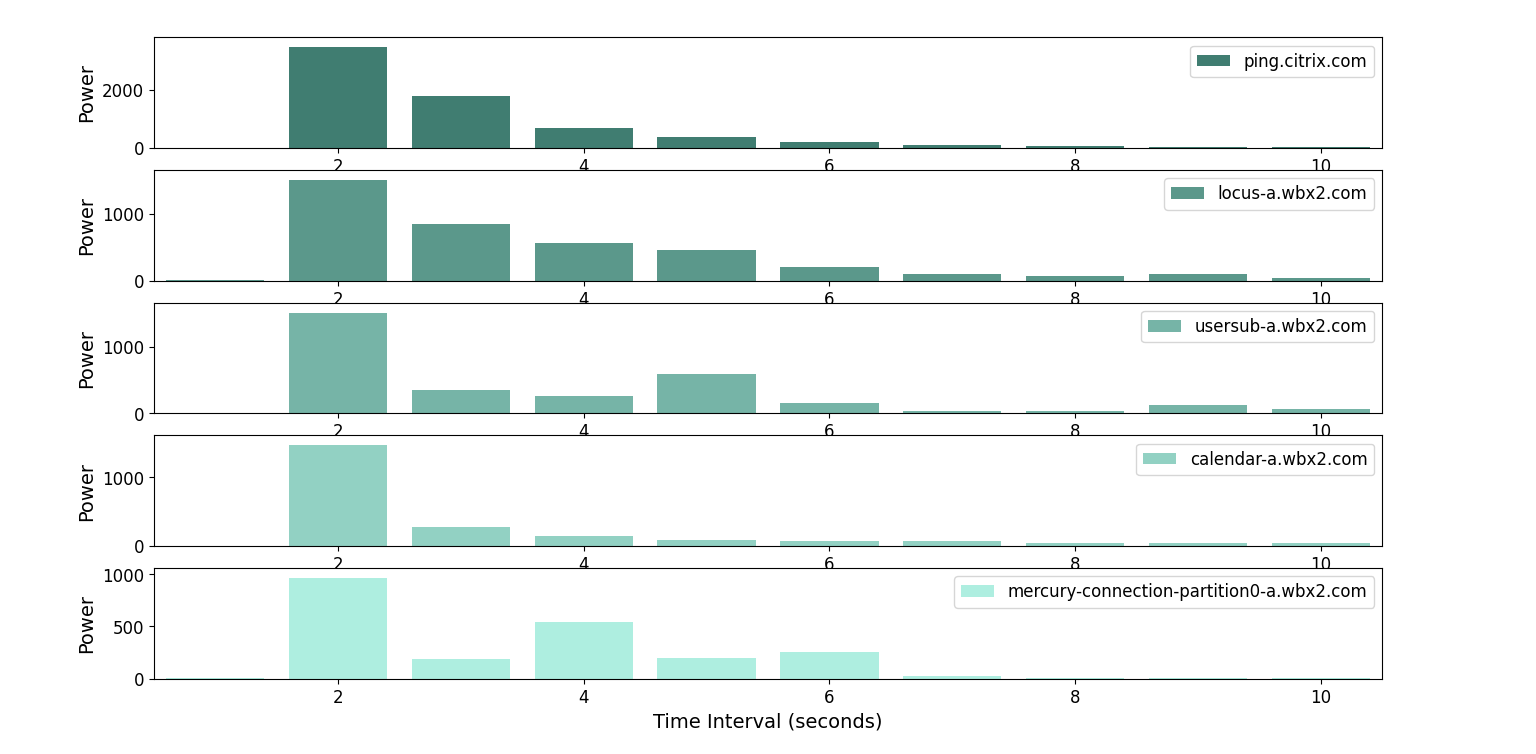
\includegraphics[width=\textwidth, height=0.5\textheight]{../Thesis_Docs/media/algorithm final output.png}
    \caption{Steps of the proposed method}
    \label{fig:final}
\end{figure}

\section{Summary}

In this chapter, we delved into the intricacies of preprocessing network activity data, focusing on the creation and utilization of a whitelist and the application of bandpass filtering to enhance data analysis. The primary learnings from this chapter include:

\begin{itemize}
    \item \textbf{Whitelist Creation:}
    \begin{itemize}
        \item We defined a function to create a whitelist by filtering out URLs based on specified exclusion criteria. This function plays a crucial role in curating a subset of URLs for further analysis, ensuring that only relevant and trustworthy URLs are retained.
        \item We discussed the importance of excluding irrelevant or untrustworthy URLs to improve the accuracy and interpretability of subsequent analyses.
        \item Performance considerations were examined, highlighting the efficiency of the whitelist creation process and its scalability for larger datasets.
    \end{itemize}
    \item \textbf{Bandpass Filtering:}
    \begin{itemize}
        \item A function for applying bandpass filtering to the power values of network activity data was introduced. This function isolates significant frequency components within a specified range, reducing noise and enhancing the clarity of the dataset.
        \item The role of bandpass filtering in refining the dataset and focusing on the most relevant data was emphasized, contributing to a more robust understanding of temporal patterns and behaviors within the network.
        \item We explored the performance implications of the filtering process and discussed potential optimizations for handling large datasets.
    \end{itemize}
    \item \textbf{Functional Analysis:}
    \begin{itemize}
        \item Both functions were defined with detailed explanations of their parameters, functionality, and performance considerations. This structured approach ensures that the functions are well-documented and easy to understand for future use and modification.
    \end{itemize}
    \item \textbf{Function to Calculate Autocorrelation:}
    \begin{itemize}
        \item Computes the autocorrelation of a time series of power values.
        \item Measures similarity between a signal and its lagged version over time.
        \item Useful for identifying patterns, periodicity, and trends in the data.
        \item Uses the acf method from the statsmodels library to compute autocorrelation values up to a specified lag.
        \item Helps detect time-dependent structures, periodicities, noise levels, and potential anomalies in the dataset.
    \end{itemize}
    
    \item \textbf{Function to Calculate Fourier Transform:}
    \begin{itemize}
        \item Performs a Fourier Transform on the time series of power values.
        \item Decomposes the time-domain signal into its frequency components.
        \item Useful for analyzing periodic behaviors or oscillations in power data.
        \item Uses the fft method from the scipy.fft library to compute the discrete Fourier transform (DFT).
        \item Provides frequencies and corresponding amplitudes, highlighting dominant frequencies and their correlation with system events or behaviors.
    \end{itemize}
\end{itemize}

\section{Next Steps}

Building on the foundational work presented in this chapter, the next steps involve:

\begin{itemize}
    \item \textbf{Implementing Additional Preprocessing Techniques:}
    \begin{itemize}
        \item Investigate and implement additional preprocessing techniques to further enhance data quality and relevance. This may include methods such as data normalization, anomaly detection, and more sophisticated filtering techniques.
    \end{itemize}
    \item \textbf{Integrating the Preprocessed Data into Analytical Models:}
    \begin{itemize}
        \item Utilize the preprocessed data in advanced analytical models to uncover deeper insights into network behavior. This could involve machine learning algorithms, statistical analyses, and other data mining techniques.
    \end{itemize}
    \item \textbf{Evaluating and Validating the Methods:}
    \begin{itemize}
        \item Perform rigorous evaluation and validation of the preprocessing methods to ensure their effectiveness and reliability. This includes testing the methods on different datasets and scenarios to assess their generalizability and robustness.
    \end{itemize}
    \item \textbf{Automating the Preprocessing Pipeline:}
    \begin{itemize}
        \item Develop an automated preprocessing pipeline that seamlessly integrates the whitelist creation and bandpass filtering functions. This will streamline the data preparation process, making it more efficient and scalable for real-time applications.
    \end{itemize}
    \item \textbf{Documenting and Sharing Findings:}
    \begin{itemize}
        \item Document the findings and methodologies in detail to facilitate knowledge sharing and reproducibility. This includes creating comprehensive reports, code documentation, and potentially publishing the results in academic journals or conferences.
    \end{itemize}
\end{itemize}

By following these next steps, we can build upon the foundation established in this chapter, advancing our understanding and capabilities in network activity data analysis. This progression will not only enhance the accuracy and effectiveness of our analytical models but also contribute to the broader field of network security and behavior analysis.
\chapter{Experiments}
In this experimental chapter, the algorithm's capability to detect malicious data undergoes a rigorous inspection. Data from various days is collected to encompass various scenarios, ensuring a comprehensive evaluation of the algorithm's performance across different conditions. Once the data is gathered, it is processed through the algorithm to assess its ability to identify potentially harmful content. The primary focus of this chapter lies in evaluating the algorithm's effectiveness in detecting malicious content and its consistency over time. Special attention is given to the URLs flagged as suspicious by the algorithm, which are closely examined to gain deeper insights into their functionality and potential areas for enhancement. By scrutinizing these flagged URLs, the chapter aims to uncover patterns and behaviors that might indicate malicious activity, providing valuable feedback for refining the algorithm. This chapter comprehensively evaluates the algorithm's performance, utilizing real-world data to gauge its effectiveness and explore avenues for improvement. The findings from this analysis not only demonstrate the algorithm's current capabilities but also highlight opportunities for further development, ensuring its continued relevance and robustness in detecting evolving cyber threats. Through this detailed examination, the chapter aims to bolster the algorithm's ability to safeguard the network, contributing to the overall security infrastructure of the system.

\section{Validation and Testing}
To affirm the efficacy of beaconing detection, the methodology undergoes rigorous testing using diverse datasets, simulating a range of scenarios that reflect various web traffic patterns. This comprehensive validation process is undertaken to ensure that the algorithm operates reliably across different frequency ranges and adapts seamlessly to the dynamic nature of HTTP requests. By employing datasets that encompass a wide array of traffic behaviors—from normal browsing activities to more erratic patterns indicative of potential security threats—the testing aims to demonstrate the filter's robustness and versatility. Each dataset is crafted to mimic real-world conditions, providing a realistic context for evaluating the bandpass filter's performance. The results from these tests offer critical insights into the filter's ability to isolate relevant frequency components while effectively minimizing noise and irrelevant data.

Furthermore, this validation process helps in identifying any potential weaknesses or limitations of the bandpass filter, guiding subsequent refinements and optimizations. The ultimate goal is to ensure that the beaconing detection consistently enhances the accuracy and reliability of the data analysis, regardless of the variability in web traffic patterns. By confirming its adaptability and precision, this rigorous testing phase substantiates the filter's integral role in the overall methodology, cementing its contribution to the accurate detection and analysis of network behaviors.

\paragraph{Validation Steps:}
\begin{enumerate}
    \item \textbf{Diverse Datasets:} The beaconing detection is subjected to rigorous testing using datasets that exhibit varying frequencies of HTTP requests, each embodying distinct traffic patterns. These datasets are carefully curated to represent a broad range of real-world web traffic scenarios, from sporadic and unpredictable requests to highly regular and predictable beaconing activity. By employing such a diverse set of datasets, the aim is to thoroughly evaluate the filter's adaptability and effectiveness. This comprehensive approach ensures that the filter can robustly identify beaconing activity amidst different traffic environments, including those with fluctuating request intervals, mixed legitimate traffic, and potential noise. Ultimately, this testing strategy is designed to refine the beaconing detection mechanism, enhancing its accuracy and reliability across a wide array of web traffic conditions, thereby improving its practical applicability in detecting malicious or anomalous behavior in varied network contexts.
    \item \textbf{Performance Metrics:} To evaluate the method's performance, the methodology employs metrics and the preservation of relevant frequency components. These metrics serve as quantitative indicators, allowing for a thorough assessment of the filter's ability to discern and retain meaningful signal components while minimizing noise.
    \item \textbf{Real-world Scenarios:} The beaconing technique is rigorously evaluated on historical datasets containing documented instances of diverse HTTP request patterns within Allianz Company's network. This real-world testing ensures that the filter can effectively handle the complexities and nuances inherent in actual network traffic scenarios, further validating its practical utility.
\end{enumerate}

By subjecting the method to these comprehensive validation steps, the methodology aims to establish its reliability and robustness in handling a wide array of web traffic patterns. The results obtained from this testing process contribute to the confidence in the filter's performance, reinforcing its role as a valuable tool in the analysis of HTTP request patterns over time.

\subsection{In-Depth Analysis of Algorithm Output}

To assess the accuracy of the algorithm's identification of malicious behavior, a verification process was executed, which involved systematically evaluating the algorithm's outputs against known benchmarks. The initial findings from this process unveiled patterns that hinted at possible malicious behavior, indicating that the algorithm was effectively identifying anomalies consistent with malicious activities. This verification process is critical for ensuring the reliability and robustness of the algorithm in real-world applications, as it confirms the algorithm's ability to detect subtle and complex patterns indicative of potential security threats.

To further refine the focus of the analysis, Figure \ref{fig:report} provides a detailed snapshot of the data from a particular day, highlighting specific areas where suspicious activity may be present. This figure showcases the URLs identified by the algorithm, each accompanied by a distinct time interval and power level. The next critical step involves detecting the behavior of these URLs to accurately report beaconing malicious behavior. This process requires checking the power levels of these URLs against a predefined threshold value. The threshold value was selected after numerous experiments and relies heavily on the analyst's expertise and experience to ensure its accuracy and reliability.

\begin{figure}
    \centering
    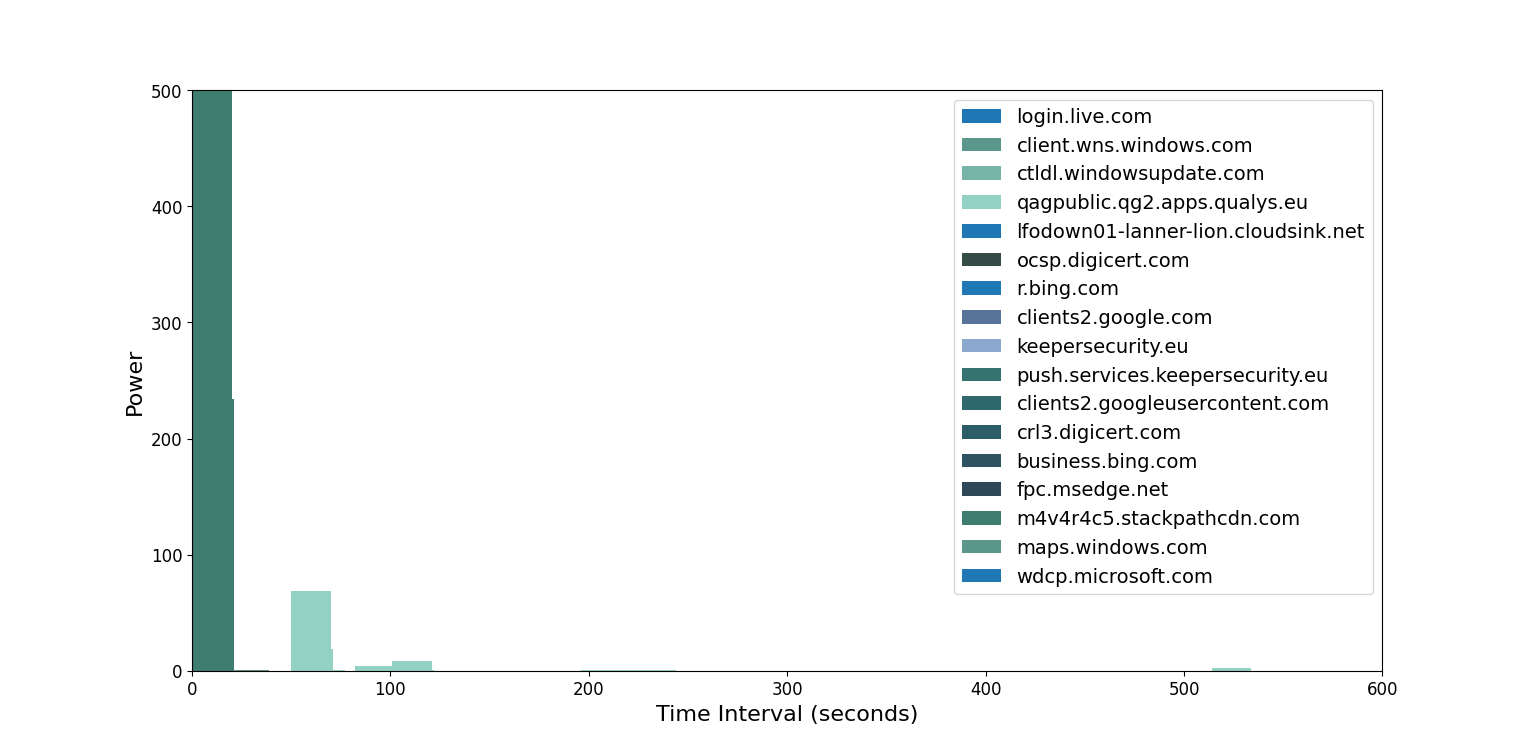
\includegraphics[width=\textwidth]{../Thesis_Docs/media/report.png}
    \caption{Testing Data}
    \label{fig:report}
\end{figure} 

To enhance clarity and isolate the most significant indicators of potential malicious activity, Figure \ref{fig:malicious} presents only those URLs that have exceeded the established threshold, which in this instance is set at 500. This strategic filtering immediately draws attention to the URL 'm4v4r4c5.stackpathcdn.com', which exhibits behavior that warrants closer scrutiny due to its elevated power levels. By isolating this particular domain from the broader dataset, the figure reveals a significant peak during a specific time interval, indicating a moment of heightened activity.

This peak is particularly noteworthy as it signifies that during the specified time interval, the power associated with 'm4v4r4c5.stackpathcdn.com' reached an unusually high value of 2877. This substantial power level is well above the predetermined threshold, clearly indicating an abnormal and potentially malicious pattern of activity. The suspicious behavior was observed within the time interval of 10-12, marking this period as a critical window for further investigation.

The isolation and examination of these peaks are important for understanding the nature of the potential threat. By focusing on the time intervals and power levels that exceed the threshold, analysts can more effectively identify and interpret patterns indicative of beaconing malicious behavior. This detailed approach underscores the importance of combining algorithmic outputs with the analyst's expertise to detect and respond to potential security threats accurately. It highlights how the rigorous verification process, alongside the use of targeted metrics and thresholds, enhances the ability to discern meaningful signals from noise, thereby improving the overall effectiveness of the beaconing detection methodology. This thorough analysis not only aids in identifying immediate threats but also contributes to the ongoing refinement of detection techniques, ensuring they remain robust and reliable in the face of evolving web traffic scenarios and potential malicious activities.

\begin{figure}
    \centering
    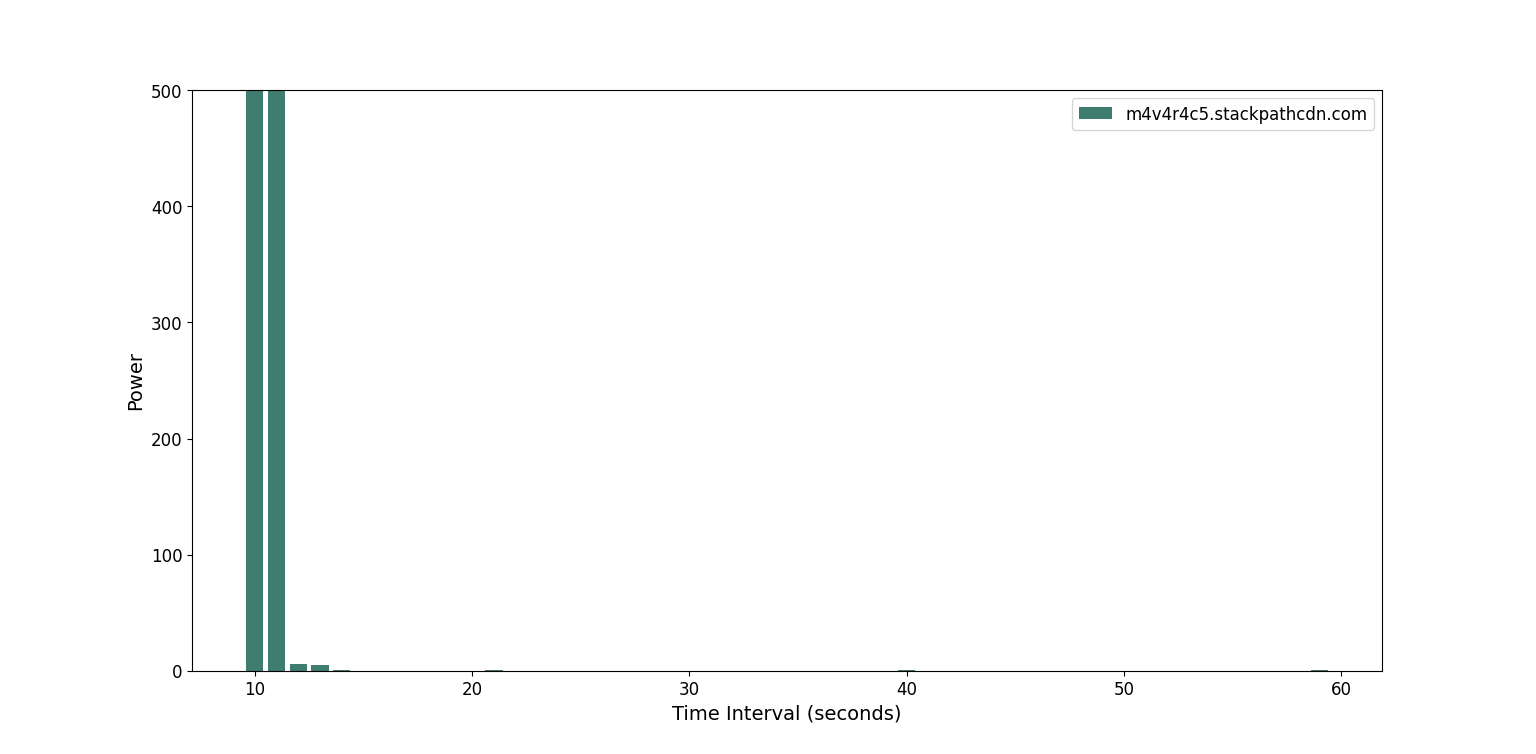
\includegraphics[width=\textwidth]{../Thesis_Docs/media/specialmalicious.png}
    \caption{Malicious Domain}
    \label{fig:malicious}
\end{figure} 

Upon the identification of the URL, the subsequent analysis unveiled clear indicators suggesting malicious intent within the algorithm's output. To verify the authenticity of these suspicions, a comprehensive inquiry was launched into the nature of the detected behavior, aimed at determining whether it unequivocally originated from a malicious URL source. This inquiry involved a detailed examination of the URL's historical footprint, which uncovered a disconcerting pattern of activity. It became evident that a particular user had persistently engaged in phishing tactics, repeatedly attempting to access and manipulate the URL for nefarious purposes. Such deliberate and systematic actions underscored the malicious nature of the user's intentions. Recognizing the severity of the situation, immediate action was taken to alert cybersecurity experts, thereby initiating a thorough examination and swift resolution of the identified security breach.

The investigation revealed that the user behind the malicious activity employed sophisticated techniques to mask their actions, making detection more challenging. This necessitated a deeper dive into the user's digital footprint, examining IP addresses, timestamps, and the nature of the requests made to the URL. The collected evidence pointed to a concerted effort to exploit vulnerabilities within the system, highlighting the importance of the initial algorithmic detection and the subsequent manual analysis in identifying and mitigating the threat.

Furthermore, to thoroughly evaluate the algorithm's effectiveness, a comprehensive analysis was conducted on the data gathered across multiple days. This longitudinal study allowed for the identification of recurring patterns or evolving trends that may signify malicious intent. The subsequent sections present the results derived from the algorithm's examination of each day's data, providing insights into the consistency and reliability of the algorithm in detecting suspicious activities. By comparing daily outputs, analysts could identify not only persistent threats but also new and emerging ones, thereby enhancing the overall security posture.

The analysis also involved cross-referencing the detected malicious activities with known threat databases to determine if the identified URL and user behavior matched any previously recorded cyber threats. This step was key in understanding the broader context of the threat and in developing appropriate countermeasures. The collaboration with cybersecurity experts ensured that the findings were promptly addressed, and preventative measures were implemented to safeguard against future attacks.

In summary, the identification of the URL and the subsequent in-depth analysis highlighted the importance of a multi-layered approach to cybersecurity. The combination of advanced algorithms, historical data analysis, and expert intervention provided a robust framework for detecting and responding to malicious activities. This approach not only addressed the immediate threat but also contributed to the ongoing refinement of detection techniques, ensuring they remain effective against evolving cyber threats.

The figures below provide comprehensive snapshots of online activity on different days, highlighting key patterns and anomalies. In the figure \ref{fig:report2}, a detailed log documents the internet activity of a specific individual on a particular day. This log outlines the various websites visited, including both innocuous sites and one that raised suspicions. The figure shows the output of an algorithm designed to detect malicious behavior, marking the beginning of a detailed analysis.

\begin{figure}
    \centering
    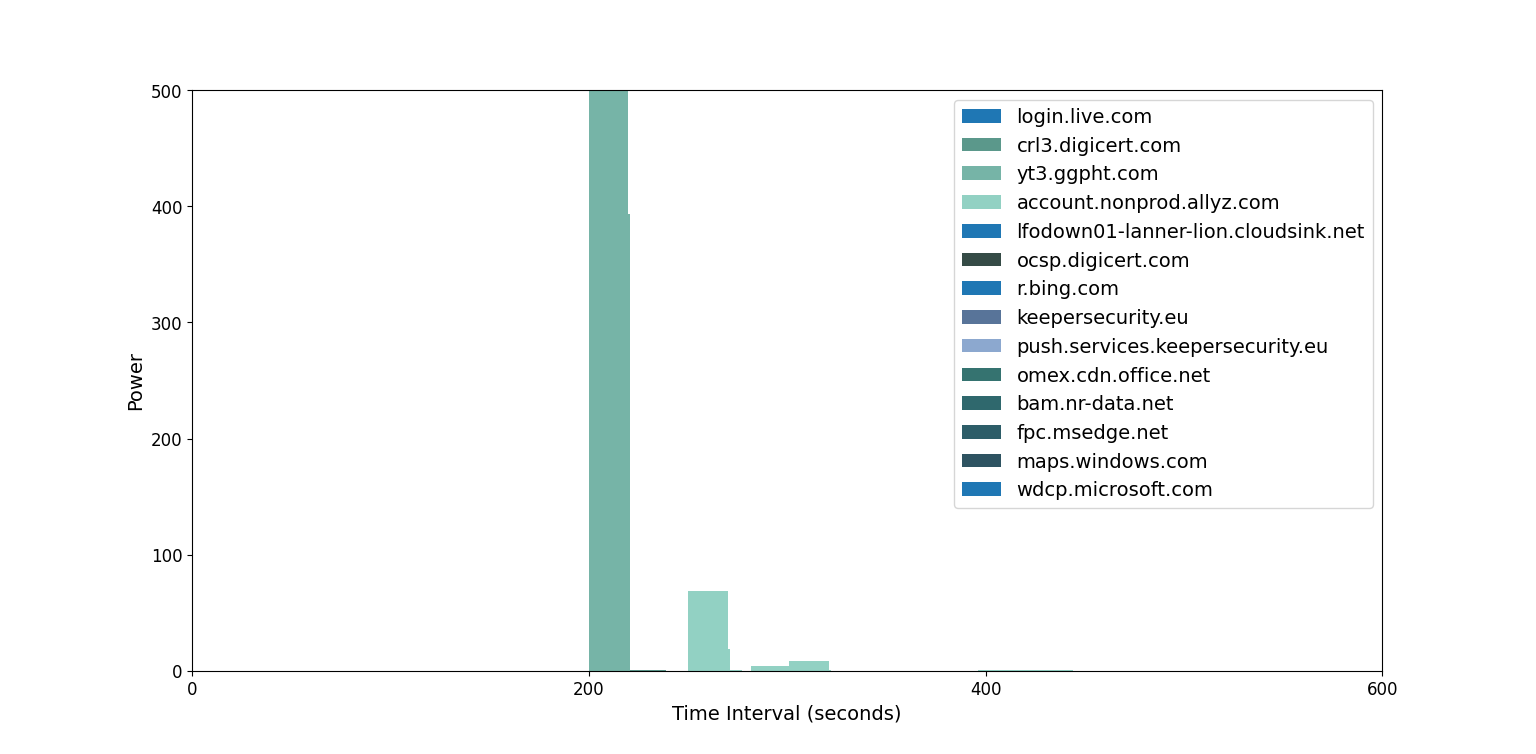
\includegraphics[width=\textwidth]{../Thesis_Docs/media/mal2.png}
    \caption{Testing Data}
    \label{fig:report2}
\end{figure} 

The focus of this analysis is to look over all URLs that exhibit a specific power level. The algorithm identifies URLs with notable peaks in the output, particularly those with power levels exceeding a predetermined threshold value. This threshold was established through extensive experimentation and expert analysis, ensuring its effectiveness in filtering out benign activity while highlighting potential threats.

Shifting the focus to Figure \ref{fig:malicious2}, this figure zooms in on a specific timeframe, offering a closer examination of a particular website's behavior. During the period from 200 to 220, there was a notable surge in activity on 'yt3.ggpht.com', which deviated significantly from its usual patterns. This irregularity prompted a deeper analysis, revealing indications of potentially malicious beaconing behavior. 

\begin{figure}
    \centering
    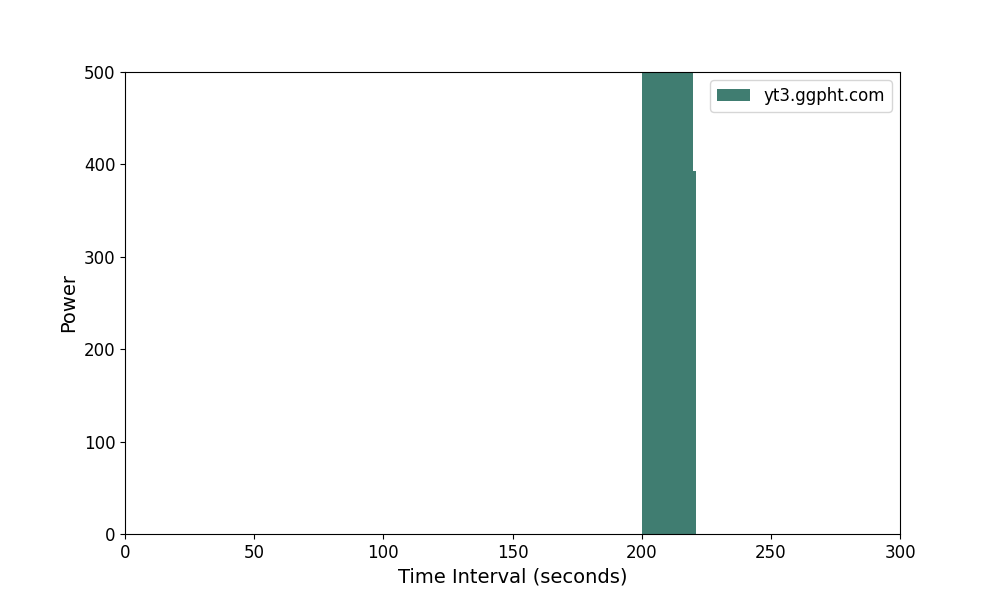
\includegraphics[width=\textwidth]{../Thesis_Docs/media/mal2s.png}
    \caption{Malicious Domain}
    \label{fig:malicious2}
\end{figure} 

The subsequent investigation into 'yt3.ggpht.com' confirmed the presence of unauthorized activity on the website. This finding underscores the critical importance of such monitoring systems in identifying and addressing cybersecurity threats. By highlighting irregular patterns and behaviors, these systems act as vigilant guardians, ensuring the safety and integrity of digital spaces. 

These visual representations play a vital role in maintaining online security. They not only facilitate the detection of malicious activity but also aid in the timely response to emerging threats. The detailed logs and focused analyses presented in Figures \ref{fig:report2} and \ref{fig:malicious2} exemplify the effectiveness of combining algorithmic detection with expert scrutiny experiences. This approach ensures that suspicious activities are not only identified but also thoroughly investigated and mitigated.

The integration of advanced algorithms and detailed visual representations provides a robust framework for monitoring and securing online environments. By continuously analyzing web traffic and identifying anomalies, these systems help protect against unauthorized activities and potential cyber threats. This multi-layered approach is  for maintaining the integrity and security of digital spaces in an increasingly connected world.

\section{Validation with Artificial Data}

To validate the proposed methodology and analysis, artificial data was generated to simulate beaconing behavior. The controlled dataset enables the exploration and understanding of patterns in the data, as well as the validation of the efficacy of the implemented algorithms, including Fast Fourier Transform (FFT) and autocorrelation analysis.The results of these analyses are visualized in Figures \ref{fig:autocorrelation10} and \ref{fig:fft_analysis}.

\subsection{Autocorrelation Analysis}

The autocorrelation function, depicted in Figure \ref{fig:auto}, provides a measure of the similarity between a time series and a time-shifted version of itself. The **x-axis** represents the **lag**, which is the time shift (in seconds) applied to the signal, while the **y-axis** represents the **autocorrelation value**, ranging from 0.0 to 1.0. A value of 1.0 indicates perfect correlation, meaning the signal aligns exactly with its shifted version, while a value of 0.0 indicates no correlation. The plot shows a sharp peak at lag zero, where the signal perfectly matches itself. As the lag increases, the autocorrelation values decay, reflecting the diminishing similarity between the signal and its shifted counterpart. This decay pattern suggests the presence of periodic behavior in the data, as the signal repeats itself at regular intervals. The gradual decline in autocorrelation values at higher lags indicates that the signal's periodicity is not perfectly regular, which is typical in real-world scenarios where noise and irregularities are present. The autocorrelation function thus serves as a powerful tool for identifying and quantifying the temporal structure of the signal.

\begin{figure}
    \centering
    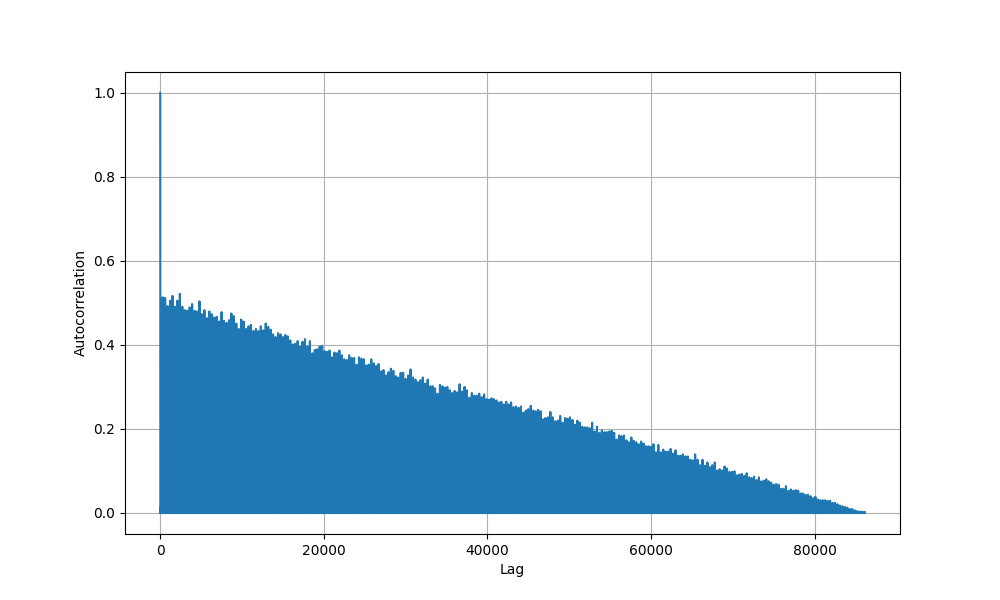
\includegraphics[width=0.8\textwidth]{../Thesis_Docs/media/auto.png}
    \caption{Autocorrelation analysis of artificially generated beaconing intervals.}
    \label{fig:autocorrelation10}
\end{figure}

\subsection{FFT Analysis}

The frequency spectrum, illustrated in Figure \ref{fig:furier}, is derived from the Fourier Transform of the time series data and reveals the distribution of signal energy across different frequencies. The **x-axis** represents the **frequency** (in Hertz), which indicates how often a periodic event occurs within the signal, while the **y-axis** represents the **amplitude**, which quantifies the strength of the signal at each frequency. The plot exhibits a dominant peak at low frequencies, indicating that the signal is primarily composed of slow, periodic oscillations. This low-frequency dominance aligns with the expected behavior of beaconing activity, where communication events occur at regular, infrequent intervals. The amplitude of the spectrum decays rapidly as the frequency increases, suggesting that high-frequency components are either absent or negligible in the signal. This spectral profile underscores the periodic nature of the data, providing a quantitative basis for identifying and characterizing the underlying temporal patterns. The frequency spectrum thus serves as a tool for uncovering the hidden periodicities in the signal, enabling the detection of beaconing behavior in network traffic.

\begin{figure}
    \centering
    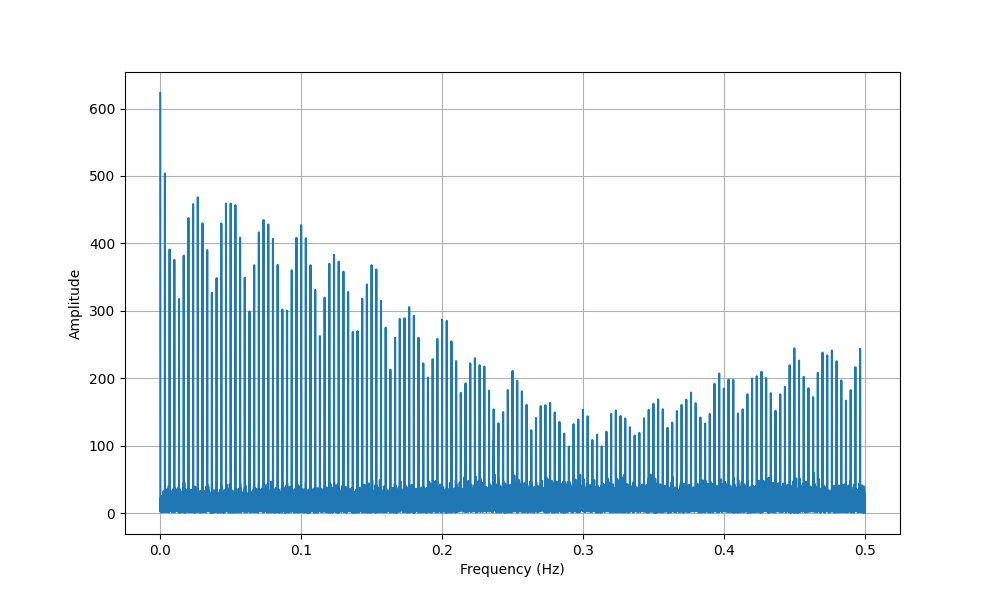
\includegraphics[width=0.8\textwidth]{../Thesis_Docs/media/furier.png}
    \caption{Fourier analysis of artificially generated beaconing intervals.}
    \label{fig:furier}
\end{figure} 

\section{Validation with Real Data}

To evaluate whether the algorithm can correctly distinguish real-world data, the Fourier Transform and Autocorrelation functions were also applied to a real non-malicious URL. The results of this analysis are presented in the figures \ref{fig:autorealdata} and \ref{fig:fourierrealdata}, where the patterns in the time domain and frequency domain can be observed. These figures provide insight into how a legitimate URL behaves over time, allowing for a direct comparison with malicious URLs. By analyzing these outputs, one can identify the characteristics of normal browsing behavior and assess whether the algorithm can successfully differentiate between benign and potentially harmful activities.

\subsection{Autocorrelation Analysis}

Figure \ref{fig:autorealdata} represents how similar the URL access pattern is when shifted over different time lags. The x-axis denotes the lag or time shift, while the y-axis indicates the autocorrelation coefficient, which measures the strength of correlation at each lag value. In the case of the non-malicious URL, the function shows a smooth decay over time rather than distinct periodic peaks. This indicates that the access pattern lacks strict periodicity and follows a more natural browsing behavior. The absence of regularly spaced peaks suggests that the accesses are not repeated at fixed intervals, making it unlikely to be generated by an automated script. Instead, the slow decrease in correlation over time implies human-driven interactions, where access intervals vary rather than being strictly uniform.

\begin{figure}
    \centering
    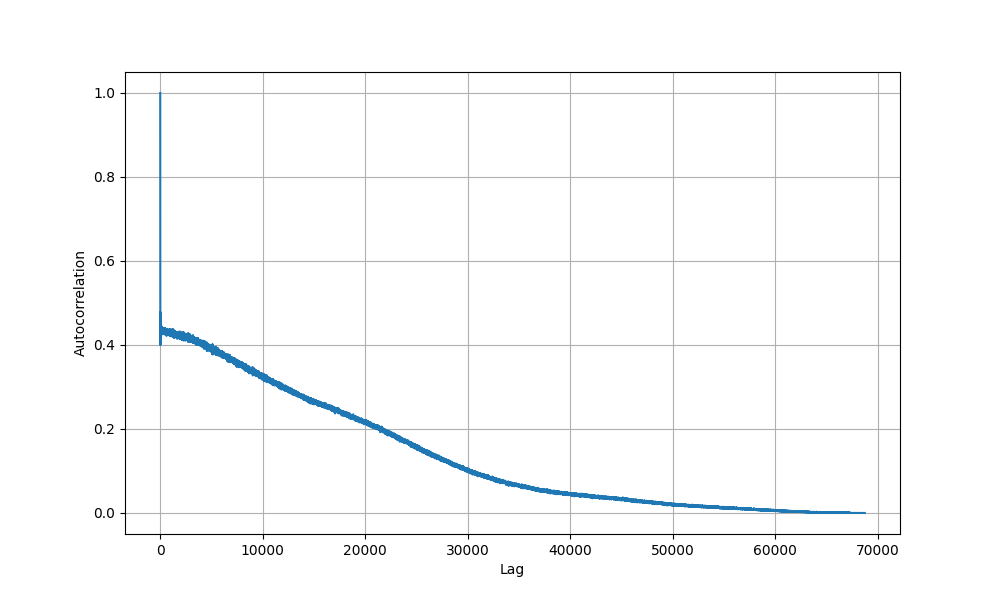
\includegraphics[width=0.8\textwidth]{../Thesis_Docs/media/auto-realdata.png}
    \caption{Autocorrelation analysis of real data}
    \label{fig:autorealdata}
\end{figure}

\subsection{FFT Analysis}

Figure \ref{fig:fourierrealdata} provides insight into its frequency components. The x-axis represents frequency, indicating how often certain access patterns repeat, while the y-axis denotes the magnitude, showing the strength of each frequency component. In this figure, the frequency spectrum appears scattered, without any dominant high-magnitude peaks. This suggests that the access behavior does not follow a strict periodic pattern. Instead, the spread-out frequency distribution indicates that the URL is accessed in an irregular, non-repetitive manner, which is characteristic of legitimate user behavior. The lack of sharp peaks further confirms that there is no automated, cyclic request pattern, reinforcing the assumption that the URL is non-malicious.

\begin{figure}
    \centering
    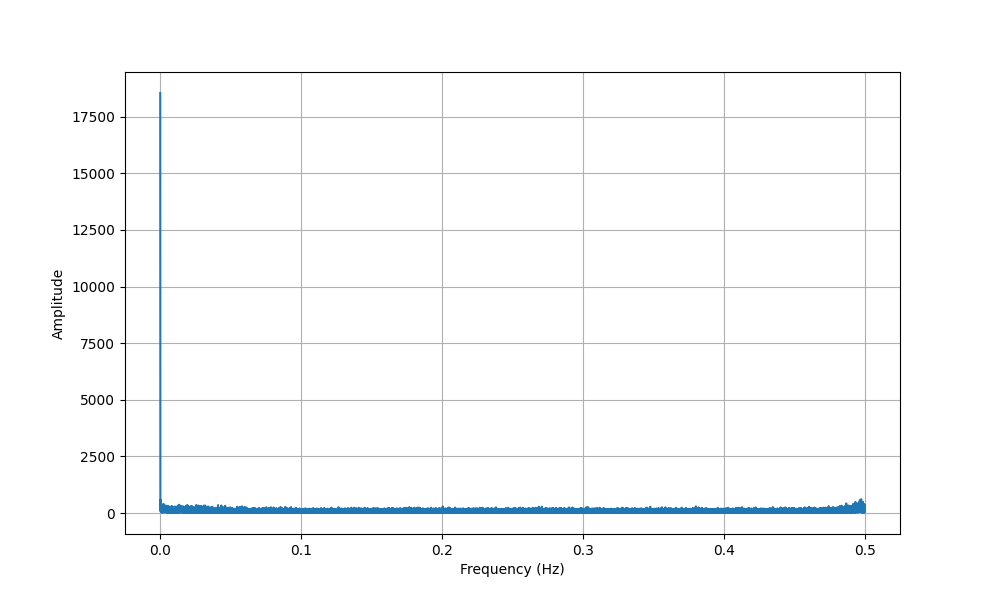
\includegraphics[width=0.8\textwidth]{../Thesis_Docs/media/fourier-realdata.png}
    \caption{Fourier analysis of real data}
    \label{fig:fourierrealdata}
\end{figure}

\chapter{Results and Discussions}
The implementation of the methodology within Allianz Company’s network infrastructure represents a pivotal advancement in enhancing network security and resilience. This chapter provides a detailed discussion of how beaconing behavior can be effectively detected and the impact of periodicity in network communication on the detection of malicious behavior. The methodology’s application involved several key steps, each contributing to the robustness of the network monitoring and security measures.

\section{Detection of Beaconing Behavior}

To address the question of how beaconing behavior can be effectively detected within Allianz Company’s network, several strategies and methodologies were employed and evaluated:

\subsection{Algorithm Development and Implementation}

The core of the detection process involved the development and implementation of advanced algorithms tailored to identify beaconing behavior. These algorithms were designed to analyze network traffic for recurring patterns indicative of beaconing. Key methods included:

\begin{itemize}
    \item \textbf{Pattern Recognition Algorithms:} These algorithms scan for regular intervals in network communication, a hallmark of beaconing activity often used by malware to maintain contact with a command-and-control server.
    \item \textbf{Threshold Analysis:} A critical component of the detection system involved setting thresholds for communication frequencies. URLs with communication intervals exceeding these thresholds were flagged for further investigation.
\end{itemize}

\subsection{Data Collection and Preprocessing}

Effective detection required comprehensive data collection and preprocessing:
\begin{itemize}
    \item \textbf{Network Monitoring:} Continuous monitoring captured a wide array of network activities, including data packets, source and destination addresses, timestamps, and communication frequencies.
    \item \textbf{Filtering and Aggregation:} Known benign traffic was filtered out, and similar types of communication were aggregated to reduce noise and focus on potentially malicious activities.
\end{itemize}

\subsection{Validation and Testing}

To ensure the effectiveness of the detection methods:
\begin{itemize}
    \item \textbf{Synthetic and Real-World Data:} The algorithm was tested on both synthetic datasets and real-world traffic from Allianz’s network.
    \item \textbf{Integration with Existing Systems:} The detection mechanisms were integrated with Security Information and Event Management (SIEM) systems to enable automated alerts and responses, and incident response teams were notified for further investigation.
\end{itemize}

\section{Impact of Periodicity in Network Communication}

The second research question addresses the impact of periodicity in network communication on the detection of malicious behavior. Periodicity significantly affects detection capabilities, as detailed below:

\subsection{Identification of Regular Intervals}

\begin{itemize}
    \item \textbf{Time-Series Analysis:} Network traffic was analyzed as time-series data to detect regular communication intervals. Techniques such as bandpass filtering was employed to identify periodic patterns.
    \item \textbf{Baseline Establishment:} A baseline of normal network behavior was established to identify deviations that might indicate malicious activity. Communication frequencies that deviated from this baseline were flagged as suspicious.
\end{itemize}

\subsection{Differentiation Between Benign and Malicious Periodicity}

\begin{itemize}
    \item \textbf{Contextual Analysis:} Not all periodic communications are indicative of malicious behavior. Contextual analysis helped distinguish between normal periodic activities (e.g., scheduled updates) and potentially harmful beaconing.
    \item \textbf{Anomaly Detection Algorithms:} Algorithms trained on periodicity patterns of normal traffic helped identify anomalies. Techniques such as clustering and classification were used to differentiate benign from malicious behavior.
\end{itemize}

\subsection{Impact on False Positives and Negatives}

\begin{itemize}
    \item \textbf{Reduction of False Positives:} Accurate modeling of normal periodic patterns helped reduce the number of false positives, ensuring that alerts were actionable.
    \item \textbf{Handling False Negatives:} Sensitivity adjustments in detection algorithms ensured that subtle periodic patterns associated with stealthy beaconing were not missed, minimizing false negatives.
\end{itemize}

\subsection{Case Studies and Empirical Evidence}

\begin{itemize}
    \item \textbf{Real-World Examples:} Analysis of real-world cases of beaconing behavior provided empirical evidence on the effectiveness of periodicity-based detection methods.
    \item \textbf{Continuous Learning and Adaptation:} The detection system was designed to adapt to evolving patterns of network traffic, ensuring ongoing effectiveness in identifying new and emerging threats.
\end{itemize}

The comprehensive evaluation of the methodology demonstrated its efficacy in handling diverse network traffic scenarios and real-world cybersecurity challenges. The methodology, which included advanced algorithms for detecting beaconing behavior, robust data preprocessing techniques, and the use of periodicity in network communication, proved effective in identifying and mitigating malicious activities. The integration of these methods with Allianz Company’s existing security infrastructure highlighted the importance of continuous monitoring and proactive response strategies in maintaining network security. The promising results from this implementation provide a strong foundation for future research and further enhancement of network security measures.
\chapter{Conclusion and Future Work}
\section{Conclusion}

The thorough study of the dataset provided valuable insights into network security, particularly in the detection of beaconing activities that may indicate potential threats. This examination involved a deep dive into the data, encompassing its various aspects and collection methods, which laid a solid foundation for understanding how networks can detect and respond to suspicious signals effectively.

Systematic data collection, cleaning, and processing were important to ensuring the dataset’s accuracy and reliability. The gathering of relevant information, removal of inconsistencies or errors, and careful preparation for analysis were  steps that validated the conclusions drawn from the data. These steps ensured that the findings were both accurate and actionable.

A significant component of the methodology was the implementation of a "whitelist" mechanism alongside specialized filtering and analysis techniques. The whitelist, which consists of trusted entities or activities within the network, plays an important role in focusing attention on potentially harmful signals while minimizing the impact of irrelevant noise. This strategic filtering enhanced the network’s ability to detect threats more effectively by isolating and addressing only the potentially malicious activities.

The evaluation of time intervals between actions, combined with data enhancement techniques and specialized filtering methods, yielded valuable insights into potential malicious beaconing activity. These analyses illuminated underlying patterns and behaviors within the network, aiding in the identification of anomalies that could signify suspicious or harmful actions. The study highlighted the importance of proactive monitoring and response strategies in mitigating cybersecurity risks, demonstrating the broader significance of data-driven methodologies in fortifying network security.

In an era where organizations face increasingly sophisticated cyber threats, the insights from this research can guide strategic decision-making and resource allocation. By leveraging these findings, organizations can enhance their protection of critical digital assets and bolster their defenses against evolving threats.

\section{Future Work}

Building on the findings and methodology presented in this study, several promising avenues for future research and development can be explored:

\begin{enumerate}
    \item \textbf{Enhanced Detection Algorithms:} Refining and optimizing beaconing detection algorithms can significantly improve accuracy and reduce false positives. Future research could explore novel approaches, such as deep learning techniques, which may provide new insights into anomaly detection in network behavior. These advancements could lead to more effective threat mitigation strategies and enhanced detection capabilities.

    \item \textbf{Real-Time Monitoring Solutions:} Investigating real-time monitoring solutions can enable prompt detection and response to emerging threats, thereby minimizing potential damages caused by malicious activities. The development of automated response mechanisms could streamline incident response procedures, reducing the burden on cybersecurity personnel and enhancing the overall efficiency of threat management.

    \item \textbf{Behavioral Analysis Across Diverse Networks:} Extending the study to analyze network behavior across a variety of organizational networks can reveal commonalities and variations in malicious activities. Understanding the unique challenges faced by different industries and sectors could lead to the development of tailored security measures that address specific threats more effectively. This cross-network analysis could provide valuable insights into how different environments respond to and manage cybersecurity risks.

    \item \textbf{Integration with Machine Learning Techniques:} Exploring the integration of advanced machine learning techniques for anomaly detection can augment the capabilities of beaconing detection systems. Leveraging historical data and learning from past incidents can help these systems adapt to evolving cybersecurity threats, enhancing proactive defense mechanisms. Machine learning models can be trained to recognize subtle patterns and adapt to new types of attacks, improving overall detection and response.

    \item \textbf{Collaborative Research Initiatives:} Engaging in collaborative research with industry partners and cybersecurity experts can foster innovation and the development of proactive security solutions. Joint research initiatives can facilitate the exchange of knowledge and resources, addressing complex cybersecurity challenges more effectively. Collaboration can lead to the creation of comprehensive solutions that benefit from diverse expertise and perspectives, driving progress in the field of network security.
\end{enumerate}

Pursuing these avenues for future research and development will help advance the field of cybersecurity, strengthening defenses against emerging threats and safeguarding the integrity of digital infrastructures. By continuing to innovate and adapt, the cybersecurity community can better protect critical assets and respond to the dynamic landscape of cyber threats.

\appendix % Start the appendix section
\lstset{ 
  language=Python, 
  basicstyle=\ttfamily\footnotesize, % Set the basic font style and size
  keywordstyle=\color{blue},         % Set the color for keywords
  stringstyle=\color{red},           % Set the color for strings
  commentstyle=\color{green},        % Set the color for comments
  numbers=left,                      % Add line numbers to the left
  numberstyle=\tiny\color{gray},     % Line number style
  stepnumber=1,                      % Line number step
  frame=single,                      % Add a frame around the code
  breaklines=true,                   % Automatic line breaking
  tabsize=4,                         % Set tab size to 4 spaces
  captionpos=b,                      % Position of the caption
  literate={
    {`}{{\textasciigrave}}1        % Handle backticks (optional)
    {`}{{\textasciigrave}}1        % Handle backticks (optional)
    {\{}{{\textbraceleft}}1        % Handle opening brace
    {\}}{{\textbraceright}}1       % Handle closing brace
    {\_}{{\_}}1                    % Handle underscore
    {>=}{{\textgreater=}}2        % Handle greater-than or equal
    {<}{{\textless}}1             % Handle less-than
    {>}{{\textgreater}}1          % Handle greater-than
    % Add more symbols here if needed
  }
}
\chapter{Appendix} % Appendix chapter title

\section{Algorithm Implementation} % Appendix section title

% Insert your Python code here
\begin{lstlisting}
from influxdb_client import InfluxDBClient
from datetime import datetime
import pandas as pd
import matplotlib.pyplot as plt
from scipy.signal import butter, filtfilt

# Function to calculate request power
def calculate_request_power(request_list):
    power_dictionary = {}
    last_date_time = request_list[0]["_time"]

    for request_dict in request_list:
        current_date_time = request_dict["_time"]

        # Check if current_date_time is a string, and convert it to a datetime object
        if isinstance(current_date_time, str):
            current_date_time = datetime.strptime(current_date_time, "%Y-%m-%dT%H:%M:%S.%fZ")

        time_delta = int((current_date_time - last_date_time).total_seconds())

        # Add the power to the power dictionary
        power_dictionary[time_delta] = power_dictionary.get(time_delta, 0) + 1
        last_date_time = current_date_time

    # Sort the dictionary for better visualization
    power_dictionary = dict(sorted(power_dictionary.items()))

    return power_dictionary

# Function to apply bandpass filtering in terms of time
def bandpass_filter(data, lowcut_time, highcut_time, sampling_rate, order=4):
    nyquist = 0.5 * sampling_rate
    lowcut = lowcut_time / nyquist
    highcut = highcut_time / nyquist

    if lowcut >= 1 or highcut >= 1:
        raise ValueError("Digital filter critical frequencies must be 0 < Wn < 1")

    b, a = butter(order, [lowcut, highcut], btype='band')
    filtered_data = filtfilt(b, a, data)
    return filtered_data

# InfluxDB connection details
url = "http://localhost:8086"
token = "****"
org = "Student"
bucket = "Net"
influx_username = '****'
influx_password = '****'

try:
    # Create an InfluxDB client
    client = InfluxDBClient(url=url, token=token, org=org)

    # Query data from InfluxDB
    query = f'from(bucket:"{bucket}") |> range(start: 2023-08-01T00:00:00Z, stop: 2023-08-02T00:00:00Z)'
    tables = client.query_api().query(query, org=org)

    # Extract points from the result
    points = [record.values for table in tables for record in table.records]

    # Process and organize the InfluxDB data
    print("Processing InfluxDB Data:")
    extracted_influx_objects = {}

    for point in points:
        url_hostname = point.get("url_hostname")

        # Check if url_hostname is already in the dictionary
        if url_hostname not in extracted_influx_objects:
            extracted_influx_objects[url_hostname] = []

        # Append under the corresponding url_hostname
        extracted_influx_objects[url_hostname].append(point)

        # Print the extracted InfluxDB data for debugging
        print(point)

    # Create a whitelist to filter out unwanted URLs
    def create_whitelist(data, exclusion_criteria):
        whitelist = {url: requests for url, requests in data.items() if not any(exclusion in url for exclusion in exclusion_criteria)}
        return whitelist

    # Define exclusion criteria for URLs
    exclusion_criteria = ['allianz', 'res']

    # Create a whitelist based on the exclusion criteria
    whitelist = create_whitelist(extracted_influx_objects, exclusion_criteria)

    print("Filtered URLs based on whitelist:")
    for url_hostname in whitelist:
        print(url_hostname)

    # Create a table of power for each URL hostname with bandpass filtering in terms of time
    print("\nPower Table with Bandpass Filtering in Terms of Time:")
    for url_hostname, requests in whitelist.items():
        print(f"URL Hostname: {url_hostname}")
        power_dictionary = calculate_request_power(requests)

        # Print the power dictionary for debugging
        print("Power Dictionary:", power_dictionary)

        # Extract keys and values from the power dictionary
        time_intervals = list(power_dictionary.keys())
        power_values = list(power_dictionary.values())

        # Apply bandpass filtering in terms of time
        lowcut_time = 5  # 5 seconds
        highcut_time = 1000  # 1000 seconds

        # Check if there are enough elements to calculate sampling rate
        if len(time_intervals) >= 2:
            sampling_rate = 1.0 / (time_intervals[1] - time_intervals[0])  # Sampling frequency

            try:
                filtered_power_values = bandpass_filter(power_values, lowcut_time, highcut_time, sampling_rate)
            except ValueError as e:
                print(f"Error: {e}")
                filtered_power_values = power_values

            # Print the filtered power values for debugging
            print("Filtered Power Values:", filtered_power_values)

            # Calculate the average power
            average_power = sum(filtered_power_values) / len(filtered_power_values)

            # Print the average power for debugging
            print("Average Power:", average_power)

            # Subtract average power from all power values
            adjusted_power_values = [power - average_power for power in filtered_power_values]

            # Print the adjusted power values for debugging
            print("Adjusted Power Values:", adjusted_power_values)

            # Remove negative powers
            non_negative_power_values = [max(0, power) for power in adjusted_power_values]

            # Get indices for the time range of interest (5 to 1000 seconds)
            time_range_indices = [i for i, t in enumerate(time_intervals) if 5 <= t <= 1000]

            # Print the time range indices for debugging
            print("Time Range Indices:", time_range_indices)

            # Plot the adjusted data within the specified time range
            plt.plot([time_intervals[i] for i in time_range_indices], [non_negative_power_values[i] for i in time_range_indices], label=url_hostname)

    # Check if there are multiple URLs in the whitelist before creating legend
    if len(whitelist) > 1:
        plt.legend()

    plt.xlabel("Time Interval (seconds)")  # Change x-axis label
    plt.ylabel("Adjusted Power")  # Change y-axis label
    plt.title("Adjusted Power over Time")  # Change the chart title
    plt.show()

except Exception as e:
    print(f"An error occurred: {e}")
\end{lstlisting}

\section{Data Analysis Implementation} % Another appendix section title

% Insert your analysis Python code here
\begin{lstlisting}
import pandas as pd
import matplotlib.pyplot as plt
from scipy.signal import butter, filtfilt

# Function to calculate request occurrence
def calculate_request_occurrence(request_list):
    occurrence_dictionary = {}
    last_date_time = None

    for _, request_row in request_list.iterrows():
        try:
            current_date_time = pd.to_datetime(request_row["_time"])

            if last_date_time is not None:
                time_delta = int((current_date_time - last_date_time).total_seconds())

                # Add the occurrence to the occurrence dictionary
                occurrence_dictionary[time_delta] = occurrence_dictionary.get(time_delta, 0) + 1

            last_date_time = current_date_time

        except (ValueError, TypeError) as e:
            print(f"Error in row: {_}, Timestamp value: {request_row['_time']}, Error message: {e}")

    # Sort the dictionary for better visualization
    occurrence_dictionary = dict(sorted(occurrence_dictionary.items()))

    return occurrence_dictionary

# Function to apply bandpass filtering in terms of time
def bandpass_filter(data, lowcut_time, highcut_time, sampling_rate, order=4):
    nyquist = 0.5 * sampling_rate
    lowcut = lowcut_time / nyquist
    highcut = highcut_time / nyquist

    if lowcut >= 1 or highcut >= 1:
        raise ValueError("Digital filter critical frequencies must be 0 < Wn < 1")

    b, a = butter(order, [lowcut, highcut], btype='band')
    filtered_data = filtfilt(b, a, data)
    return filtered_data

# CSV file path for the cleaned and modified data
csv_file_path = r'C:\Allianz\4\1125\Modified_Beaconing.csv'

try:
    # Read data from CSV file and explicitly convert "_time" to datetime
    df = pd.read_csv(csv_file_path)
    df["_time"] = pd.to_datetime(df["_time"], format='%H:%M:%S.%f', errors='coerce')

    # Process and organize the CSV data
    print("Processing CSV Data:")
    extracted_csv_objects = {}

    for _, row in df.iterrows():
        url_hostname = row.get("url_hostname")

        # Check if url_hostname is already in the dictionary
        if url_hostname not in extracted_csv_objects:
            extracted_csv_objects[url_hostname] = []

        # Append under the corresponding url_hostname
        extracted_csv_objects[url_hostname].append(row)

        # Print the extracted CSV data for debugging
        print(row)

    # Create a whitelist to filter out unwanted URLs
    def create_whitelist(data, exclusion_criteria):
        whitelist = {url: requests for url, requests in data.items() if not any(exclusion in url for exclusion in exclusion_criteria)}
        return whitelist

    # Define exclusion criteria for URLs
    exclusion_criteria = ['allianz', 'res']

    # Create a whitelist based on the exclusion criteria
    whitelist = create_whitelist(extracted_csv_objects, exclusion_criteria)

    print("Filtered URLs based on whitelist:")
    for url_hostname in whitelist:
        print(url_hostname)

    # Create a table of occurrence for each URL hostname with bandpass filtering in terms of time
    print("\nOccurrence Table with Bandpass Filtering in Terms of Time:")
    peak_url_hostname = None
    peak_occurrence_value = 0
    for url_hostname, requests in whitelist.items():
        print(f"URL Hostname: {url_hostname}")
        occurrence_dictionary = calculate_request_occurrence(pd.DataFrame(requests))

        # Print the occurrence dictionary for debugging
        print("Occurrence Dictionary:", occurrence_dictionary)

        # Identify peak occurrence value and corresponding URL hostname
        if occurrence_dictionary:
            max_occurrence_value = max(occurrence_dictionary.values())
            if max_occurrence_value > peak_occurrence_value:
                peak_occurrence_value = max_occurrence_value
                peak_url_hostname = url_hostname

        # Extract keys and values from the occurrence dictionary
        time_intervals = list(occurrence_dictionary.keys())
        occurrence_values = list(occurrence_dictionary.values())

        # Apply bandpass filtering in terms of time
        lowcut_time = 5  # 5 seconds
        highcut_time = 1000  # 1000 seconds

        # Check if there are enough elements to calculate sampling rate
        if len(time_intervals) >= 2:
            sampling_rate = 1.0 / (time_intervals[1] - time_intervals[0])  # Sampling frequency

            try:
                filtered_occurrence_values = bandpass_filter(occurrence_values, lowcut_time, highcut_time, sampling_rate)
            except ValueError as e:
                print(f"Error: {e}")
                filtered_occurrence_values = occurrence_values

            # Print the filtered occurrence values for debugging
            print("Filtered Occurrence Values:", filtered_occurrence_values)

            # Calculate the average occurrence
            average_occurrence = sum(filtered_occurrence_values) / len(filtered_occurrence_values)

            # Print the average occurrence for debugging
            print("Average Occurrence:", average_occurrence)

            # Subtract average occurrence from all occurrence values
            adjusted_occurrence_values = [occurrence - average_occurrence for occurrence in filtered_occurrence_values]

            # Print the adjusted occurrence values for debugging
            print("Adjusted Occurrence Values:", adjusted_occurrence_values)

            # Remove negative occurrences
            non_negative_occurrence_values = [max(0, occurrence) for occurrence in adjusted_occurrence_values]

            # Get indices for the time range of interest (5 to 1000 seconds)
            time_range_indices = [i for i, t in enumerate(time_intervals) if 5 <= t <= 1000]

            # Print the time range indices for debugging
            print("Time Range Indices:", time_range_indices)

            # Plot the adjusted data within the specified time range
            plt.plot([time_intervals[i] for i in time_range_indices], [non_negative_occurrence_values[i] for i in time_range_indices], label=url_hostname)

    # Print the URL hostname with the peak occurrence
    if peak_url_hostname:
        print(f"\nURL Hostname with Peak Occurrence: {peak_url_hostname}")
        print(f"Peak Occurrence Value: {peak_occurrence_value}")

    # Check if there are multiple URLs in the whitelist before creating legend
    if len(whitelist) > 1:
        plt.legend()

    plt.xlabel("Time Interval (seconds)")  # Change x-axis label
    plt.ylabel("Adjusted Occurrence")  # Change y-axis label
    plt.title("Adjusted Occurrence over Time")  # Change the chart title
    plt.show()

except Exception as e:
    print(f"An error occurred: {e}")
\end{lstlisting}

\bibliographystyle{IEEEtran}
\bibliography{../Thesis_Docs/sources/references}
\end{document}
